% !TEX program = xelatex
\documentclass[theorem=false,mathfont=none,openany,sub3section]{easybook}

\usepackage[lang=cn]{eb-elegantbook}
\usepackage{lmodern}
\usepackage{extarrows}
\usepackage{codehigh}
\lstset{moreemph={nofont,thmenv}}

\renewcommand{\rmdefault}{lmr}
\renewcommand{\sfdefault}{lmss}
\renewcommand{\ttdefault}{lmtt}

\title{Complex Analysis}
\subtitle{Lecture Notes}
\author{Stone Sun}
\date{\today}
\bioinfo{联系方式}{hefengzhishui@outlook.com}

\setcounter{tocdepth}{3}

\logo{logo.jpg}
\cover{cover.jpg}

\newcommand{\ccr}[1]{\makecell{{\color{#1}\rule{1cm}{1cm}}}}

\definecolor{customcolor}{RGB}{32,178,170}
\definecolor{diagramorange}{RGB}{238,118,0}
\colorlet{coverlinecolor}{customcolor}
\tikzset{
  diagram axis/.style={->,>=stealth,thin,draw=black!72},
  diagram map/.style={->,>=stealth,very thick,draw=black!78},
  diagram source/.style={draw=customcolor,very thick,fill=customcolor!10},
  diagram target/.style={draw=diagramorange,very thick,fill=diagramorange!9},
  diagram point/.style={circle,fill=black,inner sep=1.7pt},
  diagram note/.style={font=\small,text=black!72}
}

\let\ls\lstinline
\ebhdrset{footnotetype=flush}
\ctexset{
  paragraph/numbering=false,
  paragraph/beforeskip=1explus.2ex
  }
\SetTocStyle{subsubsection}{sub2}{
  tocindent=3.8em,
  tocformat+=\color{blue}
  }
\UseTocStyle{subsubsection}{sub2}{toc}
\SetTocStyle{chapter}{emph}{
  tocformat+=\bfseries
  }
\UseTocStyle{chapter}{emph}{toc}

\begin{document}

\maketitle
\begin{center}
谨以此篇, 献给热爱复分析的你.\par
\end{center}
\frontmatter

\begingroup
\renewcommand{\familydefault}{\rmdefault}
\tableofcontents
\endgroup

\newpage
\begin{center}
\Large
\textbf{前言}\par
\end{center}

\hspace{2em}

这是一份关于复变函数(又名复分析)的讲义, 主要涵盖了复数与复变函数、解析函数、复变函数的积分、解析函数的幂级数展开、洛朗展式与孤立奇点、留数及其应用以及保形变换等基本概念和定理. 这份讲义是基于中国海洋大学的复变函数课程的讲义和笔记而写成的, 也参考了其他一些教材和讲义.\par
值得注意的是, 这门课程在不同开课学院的所占学分和所需学时是不同的. 所以这份讲义可能更适合每周3学时的同学学习参考.\par
这份讲义的描述角度是一位数学专业的学生, 因此我可能会采用一些更易于理解, 但不严格符合课程结构的叙述方式和顺序. 这些特性决定了这份讲义不会有太广泛的适用性.\par
笔者曾经试图撰写过常微分方程、微积分、线性代数等课程的讲义, 但由于时间和精力的限制, 这些讲义都没有完成. 这份讲义是笔者在2025年春季学期和暑期复习这门课程时完成的, 从某种程度上来讲这既是对此前未完成的讲义的一种补偿, 也是对自己本科学习生活的一份总结. 我希望在这份讲义里更多地去体现我对复分析的理解和我对分析学的认知. 尽管这些认知可能都是浅显的, 但我仍希望这些想法能够落到具体实际, 以作纪念和方便回顾.\par
除了上述这些想法之外, 我还希望基于此回忆一些学习时的一些有趣的理解, 作为一名可能对分析方向不太感兴趣的学生, 我的这份讲义可能不会带来任何有益的帮助, 反倒可能对基础分析概念的理解产生许多误解, 因此我更希望读者将这份讲义看作漫谈, 而非一份严谨的参考讲义, 同时我也很期待任何同学能够帮助我修正其中的任何错误.\par
\begin{flushright}
\text{Stone Sun}\\
\text{\today}
\end{flushright}

\mainmatter

\chapter{复数与复变函数}

\section{复数}

\subsection{复数及运算}

\begin{definition}
  虚数单位 $i$：方程 $x^{2}+1=0$ 的根 $\pm i$.
\end{definition}

\begin{definition}
  复数：$z=x+iy$, $x,y$ 均为实数.\par
  $x$ 称为 $z$ 的实部, 记作 $\operatorname{Re}z$, $y$ 称为 $z$ 的虚部, 记作 $\operatorname{Im}z$.
\end{definition}

\begin{definition}
  共轭复数：$z=x+iy$ 与 $\overline{z}=x-iy$ 互为共轭复数.
\end{definition}

\begin{definition}
  复数的模与辐角\par
  在 $xOy$ 坐标系中的点 $(x,y)$ 与复数 $z=x+iy$ 建立一一对应, 故 $xOy$ 坐标平面也可称为复平面, 复数 $z=x+iy$ 与向量 $\overrightarrow{OZ}$ 一一对应.\par
  复数的模：$z=x+iy$ 的模 $|z|$ 记作 $r=\sqrt{x^{2}+y^{2}}=|\overrightarrow{OZ}|$.\par
  复数的辐角：$\overrightarrow{OZ}$ 与 $x$ 轴的正向的夹角 $\theta$ 称为 $z$ 的辐角, 记作 $\operatorname{Arg}z$. $\operatorname{Arg}z=\arg z+2k\pi$, $k=0,\pm1,\cdots$ ($z=0$ 无辐角). 这里 $\arg z$ 指辐角主值, 经常这样规定：$-\pi<\arg z\leq\pi$，或 $0<\arg z\leq 2\pi$. 例如,
  \[
  \begin{aligned}
  z=1+i&\colon \arg z=\frac{\pi}{4},\quad
  \operatorname{Arg}z=\frac{\pi}{4}+2k\pi,\ k=0,\pm1,\cdots,\\
  z=1-i&\colon \arg z=-\frac{\pi}{4}\ \Bigl(\text{或 }\arg z=\frac{7\pi}{4}\Bigr),\quad
  \operatorname{Arg}z=\frac{7\pi}{4}+2k\pi.
  \end{aligned}
  \]
\end{definition}

\begin{example}
  已知 $z=x+iy$, 则 $(-\pi<\arg z\leq\pi)$:
  \[
  \arg z=
  \begin{cases}
    \arctan\frac{y}{x}, & x>0 \\[4pt]
    \arctan\frac{y}{x}+\pi, & x<0,\ y\geq 0 \\[4pt]
    \arctan\frac{y}{x}-\pi, & x<0,\ y<0 \\[4pt]
    \frac{\pi}{2}, & x=0,\ y>0 \\[4pt]
    -\frac{\pi}{2}, & x=0,\ y<0.
  \end{cases}
  \]
\end{example}

\subsection{复数的四则运算}

设 $z_{1}=x_{1}+iy_{1}$, $z_{2}=x_{2}+iy_{2}$, 则：
\begin{itemize}
  \item $z_{1}\pm z_{2}=(x_{1}\pm x_{2})+i(y_{1}\pm y_{2})$.
  \item $z_{1}\cdot z_{2}=(x_{1}+iy_{1})(x_{2}+iy_{2})=(x_{1}x_{2}-y_{1}y_{2})+i(x_{1}y_{2}+x_{2}y_{1})$.
  \item $\displaystyle\frac{z_{1}}{z_{2}}=\frac{x_{1}+iy_{1}}{x_{2}+iy_{2}}=\frac{(x_{1}x_{2}+y_{1}y_{2})+i(x_{2}y_{1}-x_{1}y_{2})}{x_{2}^{2}+y_{2}^{2}}$.
\end{itemize}

特别地, $z=x+iy$, $z\cdot\overline{z}=x^{2}+y^{2}$.

\begin{example}
  设 $|z_{0}|<1$, 若 $|z|<1$, 则 $\bigl|\frac{z-z_{0}}{1-\overline{z_{0}}\cdot z}\bigr|<1$.\par
  \begin{proof}
    \[
    \Bigl|\frac{z-z_{0}}{1-\overline{z_{0}}\cdot z}\Bigr|<1
    \Leftrightarrow |z-z_{0}|^{2}<|1-\overline{z_{0}}\cdot z|^{2}
    \]
    \[
    \Leftrightarrow (z-z_{0})(\overline{z}-\overline{z_{0}})<(1-\overline{z_{0}}z)(1-z_{0}\overline{z})
    \]
    \[
    \Leftrightarrow z\overline{z}+z_{0}\overline{z_{0}}-z\overline{z_{0}}-z_{0}\overline{z}
    <1-z_{0}\overline{z}-\overline{z_{0}}z+z_{0}\overline{z_{0}}z\overline{z}
    \]
    \[
    \Leftrightarrow 1-|z|^{2}-|z_{0}|^{2}+|z|^{2}|z_{0}|^{2}>0
    \]
    \[
    \Leftrightarrow (1-|z_{0}|^{2})(1-|z|^{2})>0.
    \]
    当 $|z_{0}|<1$, $|z|<1$ 时上式成立, 故原式成立.
  \end{proof}
\end{example}

\begin{remark}
  例2的结论：
  \begin{enumerate}
    \item 设 $|z_{0}|<1$, 若 $|z|>1$, 则 $\bigl|\frac{z-z_{0}}{1-\overline{z_{0}}z}\bigr|>1$.
    \item 设 $|z_{0}|<1$, 若 $|z|=1$, 则 $\bigl|\frac{z-z_{0}}{1-\overline{z_{0}}z}\bigr|=1$.
  \end{enumerate}
  综上得, 变换 $w=\frac{z-z_{0}}{1-\overline{z_{0}}z}\ (|z_{0}|<1)$ 将单位圆 $|z|<1$ 变为 $|w|<1$.\par
  单位圆周 $|z|=1$ 变为 $|w|=1$, 外部 $|z|>1$ 变为 $|w|>1$.\par
  问题：$w=\dfrac{z-z_{0}}{1-\overline{z_{0}}z}$ 是否将 $z$ 平面正好变换为 $w$ 平面？
\end{remark}

\subsection{复数的表示形式}

\begin{enumerate}
  \item $z=x+iy$: 代数形式.
  \item $z=r\cos\theta+ir\sin\theta$: 三角形式, $r=|z|$, $\theta=\arg z$.
  \item $z=r(\cos\theta+i\sin\theta)=re^{i\theta}$: 指数形式.
\end{enumerate}

\begin{remark}
  指数形式表明复数的乘、除运算满足指数运算律：
  \[
  z_{1}=r_{1}e^{i\theta_{1}},\ z_{2}=r_{2}e^{i\theta_{2}},\quad
  z_{1}\cdot z_{2}=r_{1}r_{2}e^{i(\theta_{1}+\theta_{2})},\quad
  \frac{z_{1}}{z_{2}}=\frac{r_{1}}{r_{2}}e^{i(\theta_{1}-\theta_{2})}.
  \]
\end{remark}

例如, $1+i=\sqrt{2}e^{i\frac{\pi}{4}}$, $1-i=\sqrt{2}e^{i(-\frac{\pi}{4})}=\sqrt{2}e^{i\frac{7\pi}{4}}$.

于是有：$e^{i(\theta+2k\pi)}=e^{i\theta}$, $k=0,\pm1,\cdots$

\subsection{复数的乘幂与方根}

\begin{enumerate}
  \item 乘幂：$w=z^{n}$, $z^{n}=(x+iy)^{n}=r^{n}(\cos\theta+i\sin\theta)^{n}=r^{n}e^{in\theta}$.\par
  特别地, 棣莫弗公式 (De Moivre):
  \[
  (\cos\theta+i\sin\theta)^{n}=\cos n\theta+i\sin n\theta.
  \]
  Cor.
  \[
  \cos3\theta=\cos^{3}\theta-3\cos\theta\sin^{2}\theta,\quad
  \sin3\theta=3\cos^{2}\theta\sin\theta-\sin^{3}\theta,
  \]
  \[
  (\cos\theta+i\sin\theta)^{3}
  =\cos^{3}\theta+3i\cos^{2}\theta\sin\theta-3\cos\theta\sin^{2}\theta-i\sin^{3}\theta.
  \]

  \item 方根：复数 $z$ 的 $n$ 次方根即方程 $z=w^{n}$ 的根.\par
  即求 $w=\rho e^{i\varphi}$ 满足 $z=w^{n}$:
  \[
  re^{i\theta}=\rho^{n}e^{in\varphi}\ \Rightarrow\ \rho=\sqrt[n]{r},\quad
  \varphi=\frac{\theta+2k\pi}{n},\ k=0,\pm1,\cdots
  \]
  \[
  \sqrt[n]{z}=\sqrt[n]{|z|}\,e^{\frac{\theta+2k\pi}{n}i},\quad k=0,1,\cdots,n-1.
  \]
  记 $w_{k}=(\sqrt[n]{z})_{k}=\sqrt[n]{|z|}\,e^{i\frac{\theta+2k\pi}{n}}$, $k=0,1,\cdots,n-1$.
\end{enumerate}

\begin{theorem}
  一个非零复数 $z=re^{i\theta}$ 的 $n$ 次方根有 $n$ 个值 ($f(z)=\sqrt[n]{z}$), 这 $n$ 个方根均匀落在
  $w$ 平面中半径为 $\sqrt[n]{r}$ 的圆周 $|w|=\sqrt[n]{r}$ 上.
\end{theorem}

\begin{center}
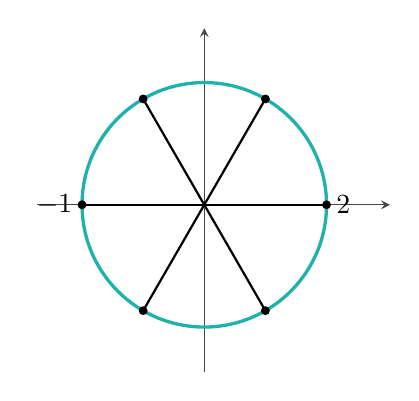
\begin{tikzpicture}[x=1.15cm,y=1.15cm,font=\normalsize]
  \draw[diagram axis] (-1.85,0)--(2.05,0);
  \draw[diagram axis] (0,-1.85)--(0,1.95);
  \draw[customcolor,very thick] (0,0) circle (1.35);
  \foreach \k in {0,...,5}{
    \draw[thick] (0,0)--({1.35*cos(60*\k)},{1.35*sin(60*\k)});
    \fill ({1.35*cos(60*\k)},{1.35*sin(60*\k)}) circle (1.6pt);
  }
  \node[left] at (-1.35,0) {$-1$};
  \node[right] at (1.35,0) {$2$};
\end{tikzpicture}
\end{center}

\begin{example}
  $\sqrt[3]{-1}=e^{i\frac{\pi+2k\pi}{3}}$, $k=0,1,2$;\quad
  $\sqrt[3]{8}=2e^{i\frac{2k\pi}{3}}$, $k=0,1,2$.
\end{example}

\begin{example}
  方程 $z^{4}+a^{4}=0\ (a>0)$ 的根: $z_{k}=ae^{i\frac{\pi+2k\pi}{4}}$, $k=0,1,2,3$.
\end{example}

\newpage

\section{复平面上的点集及曲线}

\subsection{复平面上点集}

在 $xOy$ 平面上, 点 $(x,y)$ 与一个复数 $z=x+iy$ 及向量 $\overrightarrow{Oz}$ 建立一一对应, 故 $xOy$ 平面称为复平面, $x$ 轴称为实轴, $y$ 轴称为虚轴.

下面给出复平面上有关点集的基本概念：

\begin{definition}
  $N_{\rho}(z_{0})=\{z\mid|z-z_{0}|<\rho\}$ 称为以 $z_{0}$ 为中心, $\rho$ 为半径的邻域.\par
  其余 11 个概念可由邻域定义：内点、开集、边界点及边界、闭集、连通集、开区域、闭区域、有界点集、点集的直径、聚点、孤立点.\par
  上述概念的定义完全类似二维空间中点集的概念.
\end{definition}

\subsection{复数域的完备性定理}

闭区域套定理, 柯西收敛准则, 致密性定理, 有限覆盖定理, 聚点定理.

\subsection{复数点列的收敛性}

\begin{enumerate}
  \item $\{z_{n}\}\to z_{0}\Longleftrightarrow\forall\varepsilon>0,\exists N>0$, $n>N$ 时 $|z_{n}-z_{0}|<\varepsilon$.
  \item $\{z_{n}\}$ 收敛 $\Leftrightarrow$ $\forall\varepsilon>0,\exists N>0$, $n,m>N$ 时 $|z_{n}-z_{m}|<\varepsilon$.
  \item 设 $z_{n}=x_{n}+iy_{n}$, 则 $z_{n}\to z_{0}=x_{0}+iy_{0}\Leftrightarrow x_{n}\to x_{0}, y_{n}\to y_{0}$.
\end{enumerate}

\subsection{复平面上的曲线}

在 $xOy$ 平面中, 曲线参数方程为 $L:\begin{cases}x=x(t)\\y=y(t)\end{cases},\ t\in I$. 对应在复平面上, 一般形式为 $z=x(t)+iy(t),\ t\in I$, 这里 $x(t),y(t)$ 均为实变量实函数.

\begin{definition}
  若曲线 $L:z=z(t)=x(t)+iy(t)$ 中 $x(t)$ 与 $y(t)$ 都连续, 则称曲线 $L$ 是连续曲线.
\end{definition}

\begin{definition}
  无重点的连续曲线称为简单曲线 (Jordan 曲线).\par
  曲线的重点：曲线的参数方程中不同参数对应于同一点, 这种点称为曲线的重点.
\end{definition}

\begin{definition}
  在曲线的参数方程 $z=z(t)=x(t)+iy(t)$ 中, 当 $x'(t)$ 和 $y'(t)$ 都连续且 $x'^{2}(t)+y'^{2}(t)\neq0$, 则称 $L$ 是光滑曲线.
\end{definition}

\begin{proposition}
  光滑曲线一定可求长.\par
  弧长 $S=\int_{\alpha}^{\beta}\sqrt{x'^{2}(t)+y'^{2}(t)}\,dt=\int_{\alpha}^{\beta}|z'(t)|\,dt$.
\end{proposition}

\subsection{常见平面曲线}

\begin{enumerate}
  \item 直线方程：过两点 $z_{1},z_{2}$ 的直线方程 $z=z_{1}+(z_{2}-z_{1})t$, $t\in\mathbb{R}$.
  \item 圆弧方程: $z=z_{0}+Re^{i\theta}$, $0\leq\theta<2\pi$.\par
  其他形式：$|z-z_{0}|=R$, 或 $z\overline{z}+\overline{\beta}z+\beta\overline{z}+C=0$, 这里 $C$ 为实数, 满足 $|\beta|^{2}>C$, 表示以 $-\beta$ 为圆心, $\sqrt{|\beta|^{2}-C}$ 为半径的圆.
\end{enumerate}

\newpage

\section{复变函数}

\subsection{复变函数定义及表示形式}

\begin{definition}
  设 $D$ 是复平面 $z$ 上的一个复数集, $W$ 是复平面 $w$ 上的一个复数集, 称 $D$ 到 $W$ 上的映射 $f$ 为定义在 $D$ 上的一个复变函数, 记为 $w=f(z)$, $z\in D$, $w\in W$.\par
  $D$ 称为 $f$ 的定义域, $f(D)\subset W$, $f(D)$ 称为值域.\par
  例如, $f(z)=z^{2},\ z\in D$; $f(z)=\overline{z}$; $f(z)=\sqrt[n]{z}$ (多值);\par
  $f(z)=\arg z$ (单值); $f(z)=\operatorname{Arg}z$ (多值).
\end{definition}

\begin{remark}
  复变函数可以是复变量的实值函数或实变量的复(或实)函数.
\end{remark}

\subsection{复变函数的几种表示形式}

\begin{enumerate}
  \item $w=f(z)=u(z)+iv(z)$, 这里 $u,v$ 是两个复变量实函数.
  \item $w=f(z)=u(x,y)+iv(x,y)$, 这里 $u,v$ 是两个实变量实函数.
  \item $w=f(z)=u(r,\theta)+iv(r,\theta)$.
\end{enumerate}

\subsection{复变函数的几何意义}

映射.

\begin{center}
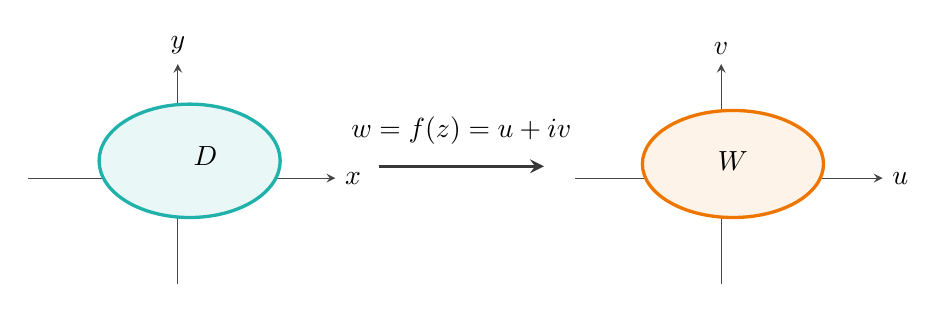
\begin{tikzpicture}[x=1cm,y=1cm,font=\normalsize]
  \draw[diagram axis] (-5.6,0)--(-1.7,0) node[right] {$x$};
  \draw[diagram axis] (-3.7,-1.35)--(-3.7,1.45) node[above] {$y$};
  \draw[diagram source] (-3.55,0.22) ellipse (1.15 and 0.72);
  \node at (-3.35,0.28) {$D$};

  \draw[diagram map] (-1.15,0.15)--(0.95,0.15)
    node[midway,above=4pt] {$w=f(z)=u+iv$};

  \draw[diagram axis] (1.35,0)--(5.25,0) node[right] {$u$};
  \draw[diagram axis] (3.2,-1.35)--(3.2,1.45) node[above] {$v$};
  \draw[diagram target] (3.35,0.18) ellipse (1.15 and 0.68);
  \node at (3.35,0.22) {$W$};
\end{tikzpicture}
\end{center}

\subsection{复变函数的极限}

\begin{definition}
  设 $z_{0}$ 是 $f(z)$ 定义域 $D$ 中的一个聚点, 若有一个 $A\in\mathbb{C}$ 使得 $\forall\varepsilon>0$, $\exists\delta>0$, 当 $|z-z_{0}|<\delta$ 且 $z\in D$ 时满足 $|f(z)-A|<\varepsilon$, 则称 $f(z)$ 当 $z\to z_{0}$, $z\in D$ 时收敛于 $A$, 记作 $\lim_{z\to z_{0},\,z\in D}f(z)=A$.
\end{definition}

\subsection{复变函数的连续性}

\begin{definition}
  若 $\lim_{z\to z_{0},z\in D}f(z)=f(z_{0})$, 则称 $f(z)$ 在 $z_{0}$ 点连续.
\end{definition}

\begin{definition}
  若 $f(z)$ 在 $D$ 上处处连续, 则称 $f(z)$ 是 $D$ 上的连续函数.
\end{definition}

\begin{remark}
  复变函数 $f(z)$ 的定义域经常选为区域或闭区域.\par
  例如, $|z|<1$, $1<|z|<2$ 称为区域; $|z|\leq1$, $1\leq|z|\leq2$ 称为闭区域.
\end{remark}

连续的四则运算和复合函数的连续性都成立.\par
\begin{enumerate}
  \item $f(z)$ 连续 $\Rightarrow$ $|f(z)|$ 连续.
  \item $f(z)$ 连续 $\Leftrightarrow$ $\overline{f(z)}$ 连续, $|f(z)|=\sqrt{f(z)\overline{f(z)}}$.
  \item $f(z)=u(z)+iv(z)$ 连续 $\Leftrightarrow$ $u(z),v(z)$ 均连续.
  \item $f(z)=u(x,y)+iv(x,y)$ 连续 $\Leftrightarrow$ $u(x,y),v(x,y)$ 均连续.
\end{enumerate}

\begin{theorem}
  若 $f(z)$ 在有界闭区域 $D$ 上连续, 则:
  \begin{enumerate}
    \item $|f(z)|$ 有界.
    \item $|f(z)|$ 存在最大、最小值.
    \item $|f(z)|$ 能取到介于 $\max|f(z)|$ 与 $\min|f(z)|$ 间任意值.
    \item $f(z)$ 和 $|f(z)|$ 都在 $D$ 上一致连续.
  \end{enumerate}
\end{theorem}

\newpage

\section{复球面与扩充复平面}

\subsection{复平面与球面的对应}

在复平面上放一个与其相切的球面, 球面上最上方的点称为 (北) 极点, 记为 $N$. 平面上任一点 $z$ 与 $N$ 的连线, 线段与球面有唯一交点 $P$. 这样 $z$ 上的点与球面上除 $N$ 外任意点建立一一对应.\par
规定 $N$ 点也对应一个点, 记为 $\infty$. 于是球面与复平面含 $\infty$ 建立一一对应. 记复平面与 $\infty$ 的并集为扩充复平面, 即扩充复平面 $\Leftrightarrow$ 复球面.

\subsection{\texorpdfstring{关于 $\infty$ 的说明}{关于无穷远点的说明}}

\begin{enumerate}
  \item 几何意义：在复平面上 $\infty$ 可看成一个点, 例如直线经过 $\infty$, 半平面不含 $\infty$. $D:\lvert z\rvert>1$ 含 $\infty$, $\infty$ 被看作无界区域的边界点.
  \item $\infty$ 的运算性质:
  \[
  a\pm\infty=\infty,\ a\cdot\infty=\infty\ (a\neq0),\quad
  \frac{a}{\infty}=0,\ \frac{a}{0}=\infty\ (a\neq0),\ \infty\cdot\infty=\infty.
  \]
  \item 注意: $\infty\pm\infty$、$0\cdot\infty$、$\frac{0}{0}$、
  $\frac{\infty}{\infty}$ 等是不定式.
  \item $|\infty|=+\infty$: 广义实数.
  \item $z\to\infty\Leftrightarrow|z|\to+\infty$.
  \item 若 $\lim_{z\to\infty}f(z)=A$, 可记为 $f(\infty)=A$.
\end{enumerate}

\newpage

\chapter{解析函数}

\section{解析函数及 C-R 条件}

\subsection{复变函数可导与可微}

\begin{definition}
  设 $f(z)$ 在 $z_{0}$ 的某邻域内有定义, 记 $\Delta z=z-z_{0}$, $\Delta w=f(z)-f(z_{0})=f(z_{0}+\Delta z)-f(z_{0})$. 若 $\lim_{\Delta z\to0}\frac{\Delta w}{\Delta z}$ 存在, 则称 $f(z)$ 在 $z_{0}$ 处可导, 记为在 $z_{0}$ 处的导数,
  \[
  f'(z_{0})=\lim_{\Delta z\to0}\frac{\Delta w}{\Delta z}=\lim_{z\to z_{0}}\frac{f(z)-f(z_{0})}{z-z_{0}}.
  \]
\end{definition}

\begin{definition}
  若 $f(z)$ 在 $z_{0}$ 可导, 也称 $f(z)$ 在 $z_{0}$ 可微, 且微分 $dw=f'(z_{0})\Delta z$ 记作 $f'(z_{0})\,dz$.
\end{definition}

\begin{theorem}
  $f(z)$ 在 $z_{0}$ 可微 (可导) $\Leftrightarrow \Delta w=f'(z_{0})\Delta z+o(|\Delta z|)$.
\end{theorem}

\begin{proof}
  $\frac{\Delta w}{\Delta z}\to f'(z_{0})
  \Leftrightarrow \Delta w=f'(z_{0})\Delta z+\varepsilon\cdot\Delta z
  \Leftrightarrow \Delta w=f'(z_{0})\Delta z+o(|\Delta z|)$.
\end{proof}

\begin{remark}
  $o(|\Delta z|)=o(\Delta z)$.
\end{remark}

与实函数求导法则类似, 复变函数的导数也有四则运算及复合函数求导法则:
\[
(f(z)+g(z))'=f'(z)+g'(z),\quad
(f(z)\cdot g(z))'=f'(z)g(z)+f(z)g'(z),
\]
\[
\Bigl(\frac{f(z)}{g(z)}\Bigr)'=\frac{f'(z)g(z)-f(z)g'(z)}{g^{2}(z)}.
\]


\begin{example}
  证明 $f(z)=z^{n}$ 在 $z$ 平面上处处可导, 且 $f'(z)=nz^{n-1}$.\par
  \begin{proof}
    $\forall z$, $\Delta w=f(z+\Delta z)-f(z)$,
    \[
    f'(z)=\lim_{\Delta z\to0}\frac{(z+\Delta z)^{n}-z^{n}}{\Delta z}
    =\lim_{\Delta z\to0}\frac{nz^{n-1}\Delta z+\binom{n}{2}z^{n-2}(\Delta z)^{2}+\cdots+(\Delta z)^{n}}{\Delta z}=nz^{n-1}.
    \]
  \end{proof}
\end{example}

\begin{example}
  证明 $f(z)=\overline{z}$ 在全平面上处处不可导.\par
  \begin{proof}
    $\forall z$, $\Delta w=f(z+\Delta z)-f(z)=\overline{z+\Delta z}-\overline{z}=\overline{\Delta z}$,
    \[
    \frac{\Delta w}{\Delta z}=\frac{\overline{\Delta z}}{\Delta z}
    =\frac{re^{-i\theta}}{re^{i\theta}}=e^{-2i\theta}.
    \]
    $\lim_{\Delta z\to0}\frac{\Delta w}{\Delta z}$ 不存在 (与路径 $\theta$ 有关).
  \end{proof}
\end{example}

\subsection{解析函数}

\begin{definition}
  若 $f(z)$ 在区域 $D$ 上处处可导, 则称 $f(z)$ 在区域 $D$ 上解析, 也称 $f(z)$ 是区域 $D$ 上的解析函数.\par
  例如, $f(z)=a_{0}z^{n}+\cdots+a_{n-1}z+a_{n}$ 在复平面上解析; $f(z)=\overline{z}$ 不解析 (在任何区域上).
\end{definition}

\begin{definition}
  $f(z)$ 在一点 $z_{0}$ 解析: 若 $f(z)$ 在 $z_{0}$ 的某个邻域内处处可导, 则称 $f(z)$ 在 $z_{0}$ 解析.
\end{definition}

\begin{remark}
  \begin{enumerate}
    \item $f(z)$ 在 $D$ 上解析 $\Leftrightarrow$ $f(z)$ 在 $D$ 上任一点解析.
    \item $f(z)$ 在 $z_{0}$ 点解析 $\Leftrightarrow$ $f(z)$ 在 $z_{0}$ 的某邻域处处解析.
    \item $f(z)$ 在 $z_{0}$ 可导 $\nRightarrow$ $f(z)$ 在 $z_{0}$ 解析.
    \item $f(z)$ 在 $z_{0}$ 不解析但在 $z_{0}$ 任意邻域内存在解析点: 奇点.
  \end{enumerate}
\end{remark}

例如, $f(z)=\frac{1}{z}$ 在 $z\neq0$ 处都解析, $z=0$ 是奇点.

\subsection{可导函数与 C-R 条件}

考虑 $f(z)=u(x,y)+iv(x,y)$ 在 $z_{0}=x_{0}+iy_{0}$ 可导/可微与 $u,v$ 在 $(x_{0},y_{0})$ 可微的关系.

\begin{theorem}
  设 $f(z)=u(x,y)+iv(x,y)$, 则 $f(z)$ 在 $z_{0}=x_{0}+iy_{0}$ 可微 $\Leftrightarrow$ $u(x,y),v(x,y)$ 在 $(x_{0},y_{0})$ 可微, 且满足 C-R 条件:
  \[
  \frac{\partial u}{\partial x}=\frac{\partial v}{\partial y},\quad
  \frac{\partial u}{\partial y}=-\frac{\partial v}{\partial x}.
  \]
\end{theorem}

\begin{proof}
  $\Rightarrow$: $f$ 在 $z_{0}$ 可微 $\Rightarrow$ $f'(z_{0})=\lim_{\Delta z\to0}\frac{\Delta w}{\Delta z}$,
  即 $\Delta w=f'(z_{0})\Delta z+o(|\Delta z|)$.
  这里 $\Delta w=\Delta u+i\Delta v$, $\Delta z=\Delta x+i\Delta y$, $o(|\Delta z|)=\varepsilon_{1}+i\varepsilon_{2}$.
  记 $f'(z_{0})=a+ib$, 代入得
  \[
  \Delta u+i\Delta v=(a+ib)(\Delta x+i\Delta y)+\varepsilon_{1}+i\varepsilon_{2}.
  \]
  比较两边,
  \[
  \Delta u=a\Delta x-b\Delta y+\varepsilon_{1},\qquad
  \Delta v=b\Delta x+a\Delta y+\varepsilon_{2}.
  \]
  以上满足 $u,v$ 在 $(x_{0},y_{0})$ 可微的定义, 故
  \[
  \frac{\partial u}{\partial x}=\frac{\partial v}{\partial y},\qquad
  \frac{\partial u}{\partial y}=-\frac{\partial v}{\partial x}.
  \]

  $\Leftarrow$: $u,v$ 在 $(x_{0},y_{0})$ 可微且满足 C-R 方程. 记
  $\frac{\partial u}{\partial x}=\frac{\partial v}{\partial y}=a$,
  $\frac{\partial u}{\partial y}=-\frac{\partial v}{\partial x}=-b$.
  \[
  \Delta u=a\Delta x-b\Delta y+o(|\Delta z|),\qquad
  \Delta v=b\Delta x+a\Delta y+o(|\Delta z|).
  \]
  \[
  \begin{aligned}
  \Delta w=\Delta u+i\Delta v
  &=(a\Delta x-b\Delta y)+i(b\Delta x+a\Delta y)+o(|\Delta z|)\\
  &=(a+ib)(\Delta x+i\Delta y)+o(|\Delta z|).
  \end{aligned}
  \]
  故
  \[
  \lim_{\Delta z\to0}\frac{\Delta w}{\Delta z}
  =\lim_{\Delta z\to0}\Bigl[(a+ib)+\frac{o(|\Delta z|)}{\Delta z}\Bigr]=a+ib.
  \]
\end{proof}

\begin{corollary}
  $f(z)$ 可导, 则
  \[
  f'(z)=\frac{\partial u}{\partial x}+i\frac{\partial v}{\partial x}
  =\frac{\partial v}{\partial y}-i\frac{\partial u}{\partial y}.
  \]
\end{corollary}

\begin{theorem}
  $f(z)=u(x,y)+iv(x,y)$ 在 $D$ 上解析 $\Leftrightarrow$ $u(x,y)$ 与 $v(x,y)$ 在 $D$ 上可微, 且满足 C-R 条件.
\end{theorem}

\begin{proof}
  略.
\end{proof}

\begin{remark}
  判断复变函数可微的方法：(1) 求导定义; (2) 定理1.
\end{remark}

\begin{theorem}[后证]
  $f(z)=u(x,y)+iv(x,y)$ 在区域 $D$ 上解析 $\Leftrightarrow$ $u(x,y)$, $v(x,y)$ 在 $D$ 上有任意阶连续偏导数, 且满足 C-R 条件.
\end{theorem}

\begin{example}
  证明 $f(z)=z|z|$ 在全平面上处处不解析.\par
  \begin{proof}
    (1) 在 $z=0$ 处, $f'(0)=\lim\limits_{z\to0}\frac{z|z|-0}{z}=0$, 故 $f(z)$ 在 $z=0$ 处可微.\par
    (2) 当 $z=x+iy\neq0$ 时,
    \[
    f(z)=z|z|=(x+iy)\sqrt{x^{2}+y^{2}},\quad
    u=x\sqrt{x^{2}+y^{2}},\ v=y\sqrt{x^{2}+y^{2}}.
    \]
    \[
    \frac{\partial u}{\partial x}=\sqrt{x^{2}+y^{2}}+\frac{x^{2}}{\sqrt{x^{2}+y^{2}}},\quad
    \frac{\partial u}{\partial y}=\frac{xy}{\sqrt{x^{2}+y^{2}}},
    \]
    \[
    \frac{\partial v}{\partial y}=\sqrt{x^{2}+y^{2}}+\frac{y^{2}}{\sqrt{x^{2}+y^{2}}},\quad
    \frac{\partial v}{\partial x}=\frac{xy}{\sqrt{x^{2}+y^{2}}}.
    \]
    由 C-R 条件 $\frac{\partial u}{\partial x}=\frac{\partial v}{\partial y}$ 得 $x^{2}=y^{2}$, 由 $\frac{\partial u}{\partial y}=-\frac{\partial v}{\partial x}$ 得 $xy=-xy$. 当 $z\neq0$ 时处处不满足, 故处处不可微.\par
    综上, $f(z)=z|z|$ 在 $z=0$ 处可微, 但处处不解析.
  \end{proof}
\end{example}

\begin{remark}
  $f(z)=z|z|$ 在 $z=0$ 处可微但不解析: 可导 $\nRightarrow$ 解析.
\end{remark}

\subsection{调和函数}

\begin{definition}
  若 $u(x,y)$ 在 $D$ 上有二阶连续偏导数, 且满足 Laplace 方程 $\frac{\partial^{2}u}{\partial x^{2}}+\frac{\partial^{2}u}{\partial y^{2}}=0$, 则称 $u$ 是 $D$ 上的调和函数.
\end{definition}

\begin{corollary}
  若 $f(z)=u(x,y)+iv(x,y)$ 在 $D$ 上解析, 则 $u$ 与 $v$ 都是调和函数.
\end{corollary}

\begin{proof}
  由定理2, $u,v$ 满足 C-R 条件: $\frac{\partial u}{\partial x}=\frac{\partial v}{\partial y}$, $\frac{\partial u}{\partial y}=-\frac{\partial v}{\partial x}$. 即
  \[
  \frac{\partial^{2}u}{\partial x^{2}}=\frac{\partial^{2}v}{\partial x\partial y},\qquad
  \frac{\partial^{2}u}{\partial y^{2}}=-\frac{\partial^{2}v}{\partial y\partial x}.
  \]
  相加得 $\frac{\partial^{2}u}{\partial x^{2}}+\frac{\partial^{2}u}{\partial y^{2}}=0$, 表明 $u$ 是 $D$ 上的调和函数. 同理可证 $v$.
\end{proof}

\begin{definition}
  若 $u$ 与 $v$ 在 $D$ 上有一阶连续偏导数, 且满足 C-R 条件, 则称 $u$ 与 $v$ 是一对共轭调和函数.
\end{definition}

\begin{remark}
  解析函数的实、虚部函数满足 C-R 条件, 表示两者存在一定关联.
\end{remark}

\begin{example}
  已知 $u=e^{x}\cos y$, 求 $v$ 使 $f(z)=u+iv$ 解析.\par
  解: $\frac{\partial u}{\partial x}=e^{x}\cos y=\frac{\partial v}{\partial y}$, 故 $v=e^{x}\sin y+C(x)$.\par
  $\frac{\partial u}{\partial y}=-e^{x}\sin y=-\frac{\partial v}{\partial x}=-e^{x}\sin y-C'(x)$, 得 $C'(x)=0$, $C(x)=C$.\par
  所以 $v=e^{x}\sin y+C$, $f(z)=e^{x}\cos y+ie^{x}\sin y+iC=e^{z}+iC$, $C\in\mathbb{R}$.
  且 $f'(z)=\frac{\partial u}{\partial x}+i\frac{\partial v}{\partial x}=e^{x}\cos y+ie^{x}\sin y=e^{z}$.
\end{example}

\newpage

\section{初等单值解析函数}

\subsection{有理分式函数}

\begin{enumerate}
  \item $P_{n}(z)=a_{0}z^{n}+a_{1}z^{n-1}+\cdots+a_{n-1}z+a_{n}$ 在复平面上解析.
  \item $W=\frac{P_{n}(z)}{Q_{m}(z)}=\frac{a_{0}z^{n}+\cdots+a_{n}}{b_{0}z^{m}+\cdots+b_{m}}$ 在 $Q_{m}(z)\neq0$ 的点外解析.
\end{enumerate}
特别地, $(c)'=0$.

\subsection{指数函数}

\begin{definition}
  $e^{z}\stackrel{z=x+iy}{=}e^{x+iy}=e^{x}e^{iy}=e^{x}(\cos y+i\sin y)$.\par
  $|e^{z}|=e^{x}$, $\arg e^{z}=y$.
\end{definition}

定义域：复平面.

性质：
\begin{enumerate}
  \item $(e^{z})'=e^{z}$, $w=e^{z}$ 在全平面上解析.
  \item 周期性: $e^{z+2k\pi i}=e^{z}$.
  \item $e^{z_{1}+z_{2}}=e^{z_{1}}\cdot e^{z_{2}}$, $e^{z_{1}-z_{2}}=\dfrac{e^{z_{1}}}{e^{z_{2}}}$.
  \item $w=e^{z}$ 无界, $\lim\limits_{z\to\infty}e^{z}$ 不存在 ($e^{\infty}$ 无意义).
  \item 当 $z=x$ 时 $e^{z}$ 是实变量指数函数.
\end{enumerate}

\subsection{三角函数}

\begin{definition}
  \[
  \sin z=\frac{e^{iz}-e^{-iz}}{2i},\quad
  \cos z=\frac{e^{iz}+e^{-iz}}{2},\quad
  \tan z=\frac{e^{iz}-e^{-iz}}{i(e^{iz}+e^{-iz})},\quad
  \cot z=\frac{i(e^{iz}+e^{-iz})}{e^{iz}-e^{-iz}}.
  \]
\end{definition}

性质：
\begin{enumerate}
  \item $\sin z,\cos z$ 在全平面上解析, 且:
  \[
  (\sin z)'=\cos z,\ (\cos z)'=-\sin z,\ (\tan z)'=\frac{1}{\cos^{2}z},\ (\cot z)'=-\frac{1}{\sin^{2}z}.
  \]
  \item 函数的零点:
  \[
  \sin(k\pi)=0,\ \cos\Bigl(k\pi+\frac{\pi}{2}\Bigr)=0,\ \tan(k\pi)=0,\ \cot\Bigl(k\pi+\frac{\pi}{2}\Bigr)=0.
  \]
  $\cot z$ 与 $\tan z$ 都在分母不为零的点上定义且解析.
  \item $\sin(z+2k\pi)=\sin z$, $\cos(z+2k\pi)=\cos z$,
  $\tan(z+k\pi)=\tan z$, $\cot(z+k\pi)=\cot z$.
  \item $\sin z,\cos z$ 均无界.
  \item 恒等式均成立 (如 $\sin^{2}z+\cos^{2}z=1$).
\end{enumerate}

\subsection{双曲函数}

\begin{definition}
  双曲正弦: $\operatorname{sh}z=\frac{e^{z}-e^{-z}}{2}$;\quad
  双曲余弦: $\operatorname{ch}z=\frac{e^{z}+e^{-z}}{2}$;\quad
  双曲正切: $\operatorname{th}z=\frac{\operatorname{sh}z}{\operatorname{ch}z}$;\quad
  双曲余切: $\operatorname{cth}z=\frac{1}{\operatorname{th}z}$.
\end{definition}

\newpage

\section{初等多值函数}

\subsection{\texorpdfstring{幂函数 $w=z^{n}$ 的单叶性区域}{幂函数 w 等于 z 的 n 次幂的单叶性区域}}

\begin{definition}
  若 $f(z)$ 在区域 $D$ 上满足 $z_{1}\neq z_{2}\Rightarrow f(z_{1})\neq f(z_{2})$, 则称 $f(z)$ 是 $D$ 上的单叶函数.\par
  单叶函数 $\Leftrightarrow$ 双方单值对应 $\Leftrightarrow$ 像与原像一一对应.
\end{definition}

\begin{definition}
  若 $f(z)$ 在区域 $D$ 上单叶, 则称 $D$ 是 $f$ 的单叶性区域.
\end{definition}

$w=z^{n}=r^{n}e^{in\theta}=\rho e^{i\varphi}$ 将 $z$ 平面上张角为 $\alpha$ ($\alpha<\frac{2\pi}{n}$) 的角域变为 $w$ 平面张角为 $n\alpha$ 的角域.
例如, $z$ 平面上的角域 $T_{k}:\frac{2k\pi}{n}-\frac{\pi}{n}<\theta<\frac{2k\pi}{n}+\frac{\pi}{n}$ 变为 $w$ 平面去掉负实轴. 类似取 $T_{k}:\frac{2k\pi}{n}<\theta<\frac{2k\pi}{n}+\frac{2\pi}{n}$.
一般地, $T_{k}$ 均是 $z^{n}$ 的单叶性区域.
$z$ 平面上, 若区域 $D$ 上任意同心圆周上两点辐角之差小于 $\frac{2\pi}{n}$, 这种区域均为 $w=z^{n}$ 的单叶性区域.

\begin{remark}
  上面两种单叶性区域 $T_{k}$ 经常使用.
\end{remark}

\subsection{\texorpdfstring{根式函数 $w=\sqrt[n]{z}$}{复数的 n 次方根函数}}

变换 $w=\sqrt[n]{z}=\sqrt[n]{r}\,e^{i(\theta+2k\pi)/n}=\rho e^{i\varphi}$ 将 $z$ 平面上张角为 $\alpha$ 的角域变为 $w$ 平面上张角为 $\alpha/n$ 的角域.
例如, $w$ 平面上 $T_{k}:\frac{2k\pi}{n}-\frac{\pi}{n}<\varphi<\frac{2k\pi}{n}+\frac{\pi}{n}$ 对应由 $z$ 平面上去掉负实轴的角域, 类似也可有 $T_{k}:\frac{2k\pi}{n}<\varphi<\frac{2k\pi}{n}+\frac{2\pi}{n}$ 的对应.

一般地, 多值函数可以分出 $n$ 个单值函数：
\[
w_{k}=(\sqrt[n]{z})_{k}=\sqrt[n]{r}\,e^{\frac{\theta+2k\pi}{n}i},\quad k=0,1,\cdots,n-1.
\]
在平面去掉某一射线到对应 $T_{k}$ 上是单叶函数.\par
若将 $z$ 平面去掉一条连接 $z=0$ 到 $z=\infty$ 的简单曲线, 则多值函数 $w=\sqrt[n]{z}$ 可以分成 $n$ 个单叶分支.

\subsection{多值函数的支点与支割线}

\begin{definition}
  $z$ 平面上的动点绕 $z=0$ 一周回到原位置, 其在变换 $w=\sqrt[n]{z}$ 下像曲线从一支变为另一支, 在每一支中都回不到原位置, 则称 $z=0$ 为支点.
  显然 $z=\infty$ 也满足支点定义, 故 $w=\sqrt[n]{z}$ 有两个支点: $z=0$, $z=\infty$.
\end{definition}

\begin{definition}
  连接所有支点的简单曲线称为支割线.
\end{definition}

\begin{remark}
  \begin{enumerate}
    \item 支割线将 $z$ 平面割破后所得区域, 这时多值函数可分出单叶分支.
    \item $w=\sqrt{(z-1)(z-2)}$ 的支点: $z=1$, $z=2$;\\
    $w=\sqrt[3]{(z-1)(z-2)}$ 的支点: $z=1$, $z=2$, $z=\infty$.
  \end{enumerate}
\end{remark}

\subsection{根式函数分支的解析性}

\begin{theorem}
  设 $f(z)=u(x,y)+iv(x,y)$, $z=re^{i\theta}$,
  记作 $f(z)=\varphi(r,\theta)+i\psi(r,\theta)$, 则 $f(z)$ 在 $z=re^{i\theta}$ 可微
  $\Leftrightarrow$ $\varphi(r,\theta),\psi(r,\theta)$ 在 $(r,\theta)$ 可微且满足
  \[
  \frac{\partial\varphi}{\partial r}=\frac{1}{r}\frac{\partial\psi}{\partial\theta},\qquad
  \frac{\partial\psi}{\partial r}=-\frac{1}{r}\frac{\partial\varphi}{\partial\theta}.
  \]
  且 $f'(z)=\frac{\partial u}{\partial x}+i\frac{\partial v}{\partial x}
  =\frac{r}{z}\bigl(\frac{\partial\varphi}{\partial r}+i\frac{\partial\psi}{\partial r}\bigr)
  =(\cos\theta-i\sin\theta)\bigl(\frac{\partial\varphi}{\partial r}+i\frac{\partial\psi}{\partial r}\bigr)$.
\end{theorem}

\begin{proof}
  (1) $u(x,y)$ 与 $v(x,y)$ 可微 $\Leftrightarrow$ $\varphi(r,\theta)$ 与 $\psi(r,\theta)$ 可微.
  (2) $\varphi(r,\theta)=u(r\cos\theta,r\sin\theta)$, $\psi(r,\theta)=v(r\cos\theta,r\sin\theta)$,
  \[
  \frac{\partial\varphi}{\partial r}=u_{x}\cos\theta+u_{y}\sin\theta,\quad
  \frac{\partial\varphi}{\partial\theta}=u_{x}(-r\sin\theta)+u_{y}(r\cos\theta),
  \]
  \[
  \frac{\partial\psi}{\partial r}=v_{x}\cos\theta+v_{y}\sin\theta,\quad
  \frac{\partial\psi}{\partial\theta}=v_{x}(-r\sin\theta)+v_{y}(r\cos\theta).
  \]
  易知 $\left\{\begin{array}{l}u_{x}=v_{y}\\ u_{y}=-v_{x}\end{array}\right.
  \Leftrightarrow
  \left\{\begin{array}{l}\frac{\partial\varphi}{\partial r}=\frac{1}{r}\frac{\partial\psi}{\partial\theta}\\[2pt]
  \frac{\partial\psi}{\partial r}=-\frac{1}{r}\frac{\partial\varphi}{\partial\theta}\end{array}\right.$.
  (3) $f'(z)=\frac{\partial u}{\partial x}+i\frac{\partial v}{\partial x}
  =\frac{\partial\varphi}{\partial r}\frac{\partial r}{\partial x}+\frac{\partial\varphi}{\partial\theta}\frac{\partial\theta}{\partial x}
  +i\Bigl(\frac{\partial\psi}{\partial r}\frac{\partial r}{\partial x}+\frac{\partial\psi}{\partial\theta}\frac{\partial\theta}{\partial x}\Bigr)
  =(\cos\theta-i\sin\theta)\bigl(\frac{\partial\varphi}{\partial r}+i\frac{\partial\psi}{\partial r}\bigr)$.
\end{proof}

\begin{corollary}
  $w_{k}=(\sqrt[n]{z})_{k}=\sqrt[n]{r}\,e^{i\frac{\theta+2k\pi}{n}}$ 在去掉支割线的区域上单叶解析.
\end{corollary}

\begin{proof}
  记 $w_{k}=(\sqrt[n]{z})_{k}=\sqrt[n]{r}\,e^{i(\theta+2k\pi)/n}$.
  (1) 前面已证: 每个分支函数都单叶.
  (2) 下面用定理证明解析:
  \[
  w_{k}=\sqrt[n]{r}\cos\frac{\theta+2k\pi}{n}+i\sqrt[n]{r}\sin\frac{\theta+2k\pi}{n}=\varphi(r,\theta)+i\psi(r,\theta).
  \]
  易知 $\varphi,\psi$ 在定义域上可微.
  \[
  \frac{\partial\varphi}{\partial r}=\frac{1}{n}r^{\frac{1}{n}-1}\cos\frac{\theta+2k\pi}{n},\quad
  \frac{\partial\varphi}{\partial\theta}=r^{\frac{1}{n}}\Bigl(-\frac{1}{n}\sin\frac{\theta+2k\pi}{n}\Bigr),
  \]
  \[
  \frac{\partial\psi}{\partial r}=\frac{1}{n}r^{\frac{1}{n}-1}\sin\frac{\theta+2k\pi}{n},\quad
  \frac{\partial\psi}{\partial\theta}=r^{\frac{1}{n}}\cdot\frac{1}{n}\cos\frac{\theta+2k\pi}{n}.
  \]
  显然成立 $\frac{\partial\varphi}{\partial r}=\frac{1}{r}\frac{\partial\psi}{\partial\theta}$,
  $\frac{\partial\psi}{\partial r}=-\frac{1}{r}\frac{\partial\varphi}{\partial\theta}$, 即 $w_{k}$ 解析, 且
  \[
  \begin{aligned}
  \frac{dw_{k}}{dz}
  &=\frac{r}{z}\Bigl(\frac{\partial\varphi}{\partial r}+i\frac{\partial\psi}{\partial r}\Bigr)
  =\frac{r}{z}\Bigl(\frac{1}{n}r^{\frac{1}{n}-1}\cos\frac{\theta+2k\pi}{n}
  +i\frac{1}{n}r^{\frac{1}{n}-1}\sin\frac{\theta+2k\pi}{n}\Bigr)\\
  &=\frac{1}{nz}\Bigl(\sqrt[n]{r}\cos\frac{\theta+2k\pi}{n}+i\sqrt[n]{r}\sin\frac{\theta+2k\pi}{n}\Bigr)
  =\frac{w_{k}}{nz}.
  \end{aligned}
  \]
\end{proof}

\begin{example}
  已知平面去掉负实轴后多值函数 $w=\sqrt[3]{z}$ 分出三个解析分支. 若某一支满足 $w_{k}(i)=-i$, 求 $w_{k}(-i)$.\par
  解: $w_{k}=w_{k}(z)=\sqrt[3]{|z|}\,e^{i\frac{\arg z+2k\pi}{3}}$, $k=0,1,2$.\par
  $w_{k}(i)=\sqrt[3]{|i|}\,e^{i\frac{\pi/2+2k\pi}{3}}=e^{i\frac{\pi+4k\pi}{6}}$, 令其等于 $-i=e^{i\frac{3\pi}{2}}$, 解得 $k=2$.\par
  $w_{2}(-i)=\sqrt[3]{|-i|}\,e^{i\frac{-\pi/2+4\pi}{3}}=e^{i\frac{7\pi}{6}}$.
\end{example}

\begin{example}
  已知平面去掉正实轴后多值函数 $w=\sqrt[3]{z}$ 分出三个分支, 若某一支满足 $w_{k}(i)=-i$, 求 $w_{k}(-i)$.\par
  解: 此时 $\arg z\in(0,2\pi)$, $w_{k}=\sqrt[3]{|z|}\,e^{i\frac{\arg z+2k\pi}{3}}$, $k=0,1,2$.\par
  $w_{k}(i)=\sqrt[3]{1}\,e^{i\frac{\pi/2+2k\pi}{3}}$, 令其等于 $-i=e^{i\frac{3\pi}{2}}$, 解得 $k=2$.\par
  $w_{2}(-i)=e^{i\frac{3\pi/2+4\pi}{3}}=e^{i\frac{11\pi}{6}}$.
\end{example}

\subsection{对数函数}

\begin{definition}
  指数函数 $z=e^{w}$ 的反函数 $w=\operatorname{Ln}z$.
  记 $z=re^{i\theta}=|z|e^{i\theta}$, $w=u+iv$, $|z|e^{i\theta}=e^{u+iv}=e^{u}e^{iv}$,
  故 $e^{u}=|z|=r$, $u=\ln|z|=\ln r$, $v=\theta+2k\pi$.
  对数函数: $w=\operatorname{Ln}z=\ln r+i(\theta+2k\pi)$, $k=0,\pm1,\pm2,\cdots$.
  记 $\ln z=\ln r+i\theta$ 为主值支.
\end{definition}

例如,
\[
\operatorname{Ln}(-1)=\ln1+i(\pi+2k\pi)=i(2k+1)\pi,\quad
\ln(-1)=\pi i,
\]
\[
\operatorname{Ln}i=\ln1+i\Bigl(\frac{\pi}{2}+2k\pi\Bigr)=i\Bigl(2k+\frac{1}{2}\Bigr)\pi,
\]
\[
\operatorname{Ln}3=\ln3+i\cdot 2k\pi.
\]

$\operatorname{Ln}0$ 无意义.

对数函数的对应关系和单叶分支: $z$ 平面上从原点出发的射线对应原像是宽为 $2k\pi$ 的水平直线. 进而, $z$ 平面去掉一条原点出发的射线所成区域, 在变换下原像是宽为 $2\pi$ 的水平带形域. 这样, 多值对数函数 $w=\operatorname{Ln}z$ 可分出单叶分支:
\[
w_{k}=(\operatorname{Ln}z)_{k}=\ln r+i(\theta+2k\pi),\quad k=0,\pm1,\pm2,\cdots
\]

\begin{center}
\begin{tikzpicture}[x=1.1cm,y=1.05cm,font=\normalsize]
  \draw[diagram axis] (-5.0,0)--(-1.7,0) node[right] {$x$};
  \draw[diagram axis] (-3.4,-1.35)--(-3.4,1.4) node[above] {$y$};
  \draw[diagramorange,very thick] (-3.4,0)--(-1.85,0);
  \node[diagram note] at (-3.4,-1.7) {$z$ 平面（正实轴）};

  \draw[diagram map] (-1.35,0)--(1.15,0);

  \draw[diagram axis] (1.5,0)--(5.2,0) node[right] {$u$};
  \draw[diagram axis] (3.3,-1.35)--(3.3,1.4) node[above] {$v$};
  \draw[customcolor,very thick] (1.7,0.95)--(4.9,0.95)
    node[right] {$2\pi$};
  \draw[customcolor,very thick] (1.7,-0.95)--(4.9,-0.95)
    node[right] {$-2\pi$};
  \node[diagram note] at (3.3,-1.7) {$w$ 平面};
\end{tikzpicture}
\end{center}

根据支点定义, $z=0$, $z=\infty$ 是对数函数 $w=\operatorname{Ln}z$ 的两个支点, 支割线是连接 $z=0$ 到 $z=\infty$ 的任意简单曲线.

\begin{corollary}
  对数函数 $w=\operatorname{Ln}z$ 的单叶分支函数在定义域上解析.
\end{corollary}

\begin{proof}
  记 $w_{k}=(\operatorname{Ln}z)_{k}=\ln r+i(\theta+2k\pi)$, $k=0,\pm1,\cdots$.
  令 $\varphi(r,\theta)=\ln r$, $\psi(r,\theta)=\theta+2k\pi$, 显然 $\varphi,\psi$ 可微且满足极坐标 C-R 条件, 故 $w_{k}(z)$ 解析.
\end{proof}

\subsection{一般幂函数与反三角函数}

\begin{definition}
  $w=z^{\alpha}=e^{\alpha\operatorname{Ln}z}$ ($\alpha\neq0$).\par
  \begin{enumerate}
    \item $\alpha=n$, $n\in\mathbb{N}^{+}$ 时, $w=z^{n}$ 是单值函数.
    \item $\alpha=\frac{n}{m}$, $n,m\in\mathbb{N}^{+}$ 且 $n,m$ 互素, $w=z^{\frac{n}{m}}=(z^{n})^{\frac{1}{m}}$ 是 $m$ 值函数.
    \item $\alpha$ 非有理数时, $w=z^{\alpha}$ 是无穷多值函数, 例如 $w=z^{i}$, $w=z^{\pi}$.
  \end{enumerate}
\end{definition}

\begin{definition}
  $w=a^{z}=e^{z\operatorname{Ln}a}$ ($a\neq0$), $w=e^{z[\ln|a|+(\theta_{0}+2k\pi)i]}$.
  $w=a^{z}$ 是无穷多值函数, 特别地, $a=e$ 时也是无穷多值.
  前面各函数定义时所用 $e^{z}=e^{x+iy}$ 是主值支.
\end{definition}

\subsection*{反三角函数}

\begin{remark}
  对数函数的导数:
  \[
  \frac{dw_{k}}{dz}=\frac{d}{dz}\bigl((\operatorname{Ln}z)_{k}\bigr)
  =\frac{r}{z}\Bigl(\frac{\partial}{\partial r}(\ln r)+i\frac{\partial}{\partial r}(\theta+2k\pi)\Bigr)=\frac{1}{z}.
  \]
\end{remark}

\newpage

\section{习题课}

\begin{example}
  设 $w=f(z)$ 在区域 $D$ 上单叶解析, 则其反函数 $z=f^{-1}(w)$ 在 $G=f(D)$ 上也解析, 且
  \[
  \frac{df^{-1}(w)}{dw}=\frac{1}{f'(z)}.
  \]
\end{example}

\begin{proof}
  $\forall z_{0}\in D$, 记 $w_{0}=f(z_{0})\in G$, 则
  \[
  \Bigl.\frac{df^{-1}(w)}{dw}\Bigr|_{w_{0}}
  =\lim_{w\to w_{0}}\frac{f^{-1}(w)-f^{-1}(w_{0})}{w-w_{0}}
  =\lim_{w\to w_{0}}\frac{z-z_{0}}{w-w_{0}}
  =\frac{1}{\displaystyle\lim_{w\to w_{0}}\frac{w-w_{0}}{z-z_{0}}}
  =\frac{1}{f'(z_{0})}.
  \]
\end{proof}

\begin{remark}
  \begin{enumerate}
    \item 若 $D$ 是区域, 其像集 $G=f(D)$ 也是区域 ($f$ 解析).
    \item 若 $f$ 在 $D$ 上单叶解析, 则 $f'(z)\neq0$.
  \end{enumerate}
\end{remark}

\begin{example}
  设 $w=f(z)$ 在有界区域 $D$ 上单叶解析, 则 $D$ 在变换 $w=f(z)$ 下的像 $G=f(D)$ 的面积为
  \[
  A=\iint_{D}|f'(z)|^{2}\,d\sigma.
  \]
\end{example}

\begin{proof}
  记 $w=f(z)=u(x,y)+iv(x,y)$, 由解析性有 $u_{x}=v_{y}$, $u_{y}=-v_{x}$.
  \[
  G\text{ 的面积 }A=\iint_{G}du\,dv
  =\iint_{D}|J|\,dx\,dy
  =\iint_{D}(u_{x}^{2}+v_{x}^{2})\,d\sigma
  =\iint_{D}|f'(z)|^{2}\,d\sigma.
  \]
\end{proof}

\begin{example}
  设 $w=f(z)$ 在上半平面上解析 $\Leftrightarrow$ $w=\overline{f(\overline{z})}$ 在下半平面上解析.
\end{example}

\begin{proof}
  $\forall z_{0}$, $\operatorname{Im}z_{0}<0$, $f'(\overline{z_{0}})$ 存在,
  \[
  \frac{dw}{dz}\Bigr|_{z_{0}}
  =\lim_{z\to z_{0}}\frac{\overline{f(\overline{z})}-\overline{f(\overline{z_{0}})}}{z-z_{0}}
  =\overline{\lim_{z\to z_{0}}\frac{f(\overline{z})-f(\overline{z_{0}})}{\overline{z}-\overline{z_{0}}}}
  =\overline{f'(\overline{z_{0}})}.
  \]
  同理反向可证.
\end{proof}

\begin{remark}
  若 $w=f(z)$ 在上半平面上解析且 $\operatorname{Im}f(x)=0$, 则 $f(z)$ 可延拓为全平面的解析函数.
  事实上有
  \[
  F(z)=\begin{cases}
    f(z), & \operatorname{Im}z\geq0,\\[2pt]
    \overline{f(\overline{z})}, & \operatorname{Im}z\leq0.
  \end{cases}
  \]
\end{remark}

\begin{example}
  已知 $u=x^{2}+2xy-y^{2}$, 求 $v$ 使 $f(z)=u+iv$ 解析.\par
  解: $\frac{\partial u}{\partial x}=2x+2y=\frac{\partial v}{\partial y}$, 故 $v=2xy+y^{2}+C(x)$.\par
  又 $\frac{\partial v}{\partial x}=2y+C'(x)=-\frac{\partial u}{\partial y}=-(2x-2y)$, 得 $C'(x)=-2x$, $C(x)=-x^{2}+C$.\par
  所以 $v=2xy+y^{2}-x^{2}+C$, $f(z)=x^{2}+2xy-y^{2}+i(2xy+y^{2}-x^{2}+C)$, $C$ 为实常数.
\end{example}

\begin{example}
  设 $u(x,y)$ 在 $D$ 上有二阶连续偏导数且为调和函数, 复变函数 $z=f(\xi)=x+iy=x(\xi,\eta)+iy(\xi,\eta)$ 在 $\xi$ 平面上解析, 则复合函数 $u(x(\xi,\eta),y(\xi,\eta))$ 在 $G$ 上也是调和函数.
\end{example}

\begin{proof}
  由题意 $\frac{\partial^{2}u}{\partial x^{2}}+\frac{\partial^{2}u}{\partial y^{2}}\equiv0$,
  $\frac{\partial x}{\partial\xi}=\frac{\partial y}{\partial\eta}$, $\frac{\partial x}{\partial\eta}=-\frac{\partial y}{\partial\xi}$,
  且 $x,y$ 亦调和:
  \[
  \frac{\partial^{2}x}{\partial\xi^{2}}+\frac{\partial^{2}x}{\partial\eta^{2}}=0,\qquad
  \frac{\partial^{2}y}{\partial\xi^{2}}+\frac{\partial^{2}y}{\partial\eta^{2}}=0.
  \]
  \[
  \frac{\partial u}{\partial\xi}=\frac{\partial u}{\partial x}\frac{\partial x}{\partial\xi}+\frac{\partial u}{\partial y}\frac{\partial y}{\partial\xi}.
  \]
  \[
  \begin{aligned}
  \frac{\partial^{2}u}{\partial\xi^{2}}
  &=\Bigl[\frac{\partial^{2}u}{\partial x^{2}}\frac{\partial x}{\partial\xi}+\frac{\partial^{2}u}{\partial x\partial y}\frac{\partial y}{\partial\xi}\Bigr]\frac{\partial x}{\partial\xi}
  +\frac{\partial u}{\partial x}\frac{\partial^{2}x}{\partial\xi^{2}}\\
  &\quad+\Bigl[\frac{\partial^{2}u}{\partial y\partial x}\frac{\partial x}{\partial\xi}+\frac{\partial^{2}u}{\partial y^{2}}\frac{\partial y}{\partial\xi}\Bigr]\frac{\partial y}{\partial\xi}
  +\frac{\partial u}{\partial y}\frac{\partial^{2}y}{\partial\xi^{2}}.
  \end{aligned}
  \]
  同理
  \[
  \begin{aligned}
  \frac{\partial^{2}u}{\partial\eta^{2}}
  &=\Bigl[\frac{\partial^{2}u}{\partial x^{2}}\frac{\partial x}{\partial\eta}+\frac{\partial^{2}u}{\partial x\partial y}\frac{\partial y}{\partial\eta}\Bigr]\frac{\partial x}{\partial\eta}
  +\frac{\partial u}{\partial x}\frac{\partial^{2}x}{\partial\eta^{2}}\\
  &\quad+\Bigl[\frac{\partial^{2}u}{\partial y\partial x}\frac{\partial x}{\partial\eta}+\frac{\partial^{2}u}{\partial y^{2}}\frac{\partial y}{\partial\eta}\Bigr]\frac{\partial y}{\partial\eta}
  +\frac{\partial u}{\partial y}\frac{\partial^{2}y}{\partial\eta^{2}}.
  \end{aligned}
  \]
  两式相加得
  \[
  \frac{\partial^{2}u}{\partial\xi^{2}}+\frac{\partial^{2}u}{\partial\eta^{2}}
  =\Bigl(\frac{\partial^{2}u}{\partial x^{2}}+\frac{\partial^{2}u}{\partial y^{2}}\Bigr)
  \Bigl[\Bigl(\frac{\partial x}{\partial\xi}\Bigr)^{2}+\Bigl(\frac{\partial y}{\partial\xi}\Bigr)^{2}\Bigr]
  =\Bigl(\frac{\partial^{2}u}{\partial x^{2}}+\frac{\partial^{2}u}{\partial y^{2}}\Bigr)\lvert f'(\xi)\rvert^{2}=0.
  \]
\end{proof}

\begin{corollary}
  $u(z)$ 调和, $z=f(\xi)$ 解析, 则 $u(f(\xi))$ 也调和.
\end{corollary}

\begin{example}
  (1) 证明多值函数 $w=\sqrt[3]{z(1-z)}$ 的支点为: $0,1,\infty$.\par
  (2) 用正实轴割破平面后, $w=\sqrt[3]{z(1-z)}$ 分出三个分支函数 $w_{k}=(\sqrt[3]{z(1-z)})_{k}$, 已知某一支 $w_{k}$ 满足 $w_{k}(-1)<0$, 求 $w_{k}(-i)$.
\end{example}

\begin{proof}
  (1) 先证 $z=0$ 为支点: 取绕 $z=0$ 的封闭曲线 $C$ (动点 $z$ 绕 $C$ 逆时针一周), 这里 $C$ 不含 $z=1$, 则
  \[
  \Delta_{C}\arg z=2\pi,\quad \Delta_{C}\arg(1-z)=0,
  \]
  \[
  \Delta_{C}\arg\sqrt[3]{z(1-z)}=\frac{2\pi+0}{3}=\frac{2\pi}{3}.
  \]
  $C$ 的像曲线没有回到原位置, 故 $z=0$ 为支点. 同理 $z=1$ 也是支点.\par
  考虑 $z=\infty$: 取顺时针方向的大圆周 $C$ (内含 $z=0$, $z=1$),
  \[
  \Delta_{C}\arg\sqrt[3]{z(1-z)}=\frac{-2\pi-2\pi}{3}=-\frac{4\pi}{3}\neq0,
  \]
  因此 $z=\infty$ 也是支点.\par
  (2) 设 $z=r_{1}e^{i\theta_{1}}$, $1-z=r_{2}e^{i\theta_{2}}$, 则
  \[
  w_{k}=\sqrt[3]{z(1-z)}=\sqrt[3]{r_{1}r_{2}}\,e^{i\frac{\theta_{1}+\theta_{2}+2k\pi}{3}},\quad k=0,1,2.
  \]
  若 $w_{k}(-1)=\sqrt[3]{2}\,e^{i\frac{\pi+0+2k\pi}{3}}<0$, 解得 $k=1$.\par
  则 $w_{1}(-i)=\sqrt[6]{2}\,e^{i\frac{3\pi/2+\pi/4+2\pi}{3}}=\sqrt[6]{2}\,e^{i\frac{15\pi}{12}}$.
\end{proof}

\begin{example}
  已知 $w=\sqrt{z(z-1)}$ 去掉正实轴上线段 $[0,1]$ 分出两个分支函数 $w_{k}=(\sqrt{z(z-1)})_{k}$, 已知某一支 $w_{k}$ 满足 $w_{k}(-1)>0$, 求 $w_{k}(-i)$.
\end{example}

\begin{proof}
  $z=0$, $z=1$ 为支点, $z=\infty$ 非支点.
  设 $z=r_{1}e^{i\theta_{1}}$, $z-1=r_{2}e^{i\theta_{2}}$, 则
  \[
  w_{k}=\sqrt{r_{1}r_{2}}\,e^{i\frac{\theta_{1}+\theta_{2}+2k\pi}{2}},\quad k=0,1.
  \]
  若 $w_{k}(-1)=\sqrt{2}\,e^{i\frac{\pi+\pi+2k\pi}{2}}>0$, 解得 $k=1$.\par
  则 $w_{1}(-i)=\sqrt[4]{2}\,e^{i\frac{3\pi/2+5\pi/4+2\pi}{2}}
  =\sqrt[4]{2}\,e^{i\frac{3\pi}{8}}$.
\end{proof}

\newpage

\chapter{复变函数的积分}

\section{复变函数积分的定义及计算法}

\subsection{复积分的定义}

\begin{definition}
  设 $C$ 是平面上一条光滑或分段光滑的有向曲线段, $a,b$ 是 $C$ 的起终点, $f(z)$ 在 $C$ 上定义. 将 $C$ 从 $a$ 到 $b$ 分成 $n$ 个有向小弧段 $\widehat{z_{0}z_{1}},\cdots,\widehat{z_{n-1}z_{n}}$, 记 $\Delta z_{i}=z_{i}-z_{i-1}$, 记 $\lambda$ 为这 $n$ 个小弧段的最大直径, 任取一点 $\zeta_{i}\in\widehat{z_{i-1}z_{i}}$, 作乘积 $f(\zeta_{i})\Delta z_{i}$, 作和式 $\sum_{i=1}^{n}f(\zeta_{i})\Delta z_{i}$. 若当 $\lambda\to0$ 时, 该和式的极限存在且与分法无关, 则称此极限为 $f(z)$ 沿 $C$ 的积分, 记作 $\int_{C}f(z)\,dz$, 否则称 $f(z)$ 不可积.
\end{definition}

\begin{remark}
  (1) 复积分本质上也是 Riemann 积分, 当 $f(z)$ 在 $C$ 上有界且几乎处处连续时可积. 可积函数一定有界.

  (2) 若 $C$ 是闭曲线, 常记为 $\oint_{C}f(z)\,dz$.
\end{remark}

\subsection{用定义计算复积分}

\begin{example}
  (1) $\int_{C}dz=b-a$; (2) $\int_{C}z\,dz=\frac{1}{2}(b^{2}-a^{2})$, 这里 $a,b$ 是 $C$ 的起终点.
  \begin{proof}
    (1) $f(z)=1$ 连续, 任意分法 $\Delta z_{i}=z_{i}-z_{i-1}$, 作和 $\sum_{i=1}^{n}1\cdot\Delta z_{i}=z_{n}-z_{0}=b-a$, 令 $\lambda\to0$, $\int_{C}dz=b-a$.

    (2) $f(z)=z$ 连续, 取 $\zeta_{i}=z_{i}$ 或 $\zeta_{i}=z_{i-1}$, 则:
    \[
    \sum_{i=1}^{n}f(z_{i})\Delta z_{i}+\sum_{i=1}^{n}f(z_{i-1})\Delta z_{i}
    =\sum_{i=1}^{n}(z_{i}^{2}-z_{i-1}^{2})=z_{n}^{2}-z_{0}^{2}=b^{2}-a^{2},
    \]
    令 $\lambda\to0$, $\int_{C}z\,dz=\frac{1}{2}(b^{2}-a^{2})$.
  \end{proof}
\end{example}

\subsection{复积分的计算法}

\begin{theorem}
  设 $f(z)=u(x,y)+iv(x,y)$ 在光滑或分段光滑的有向曲线 $C$ 上连续, 则
  \[
  \int_{C}f(z)\,dz=\int_{C}(u\,dx-v\,dy)+i\int_{C}(v\,dx+u\,dy).
  \]
\end{theorem}

\begin{proof}
  任意给定分法 $\widehat{z_{i-1}z_{i}}$, $\Delta z_{i}=z_{i}-z_{i-1}$, 记 $z_{i}=x_{i}+iy_{i}$, 则 $\Delta z_{i}=\Delta x_{i}+i\Delta y_{i}$, 任取 $\zeta_{i}=\xi_{i}+i\eta_{i}\in\widehat{z_{i-1}z_{i}}$.
  比较等式两边积分的和:
  \[
  \begin{aligned}
  \sum_{i=1}^{n}f(\zeta_{i})\Delta z_{i}
  &=\sum_{i=1}^{n}[u(\xi_{i},\eta_{i})+iv(\xi_{i},\eta_{i})]\cdot[\Delta x_{i}+i\Delta y_{i}]\\
  &=\sum_{i=1}^{n}[u(\xi_{i},\eta_{i})\Delta x_{i}-v(\xi_{i},\eta_{i})\Delta y_{i}]
    +i\sum_{i=1}^{n}[u(\xi_{i},\eta_{i})\Delta y_{i}+v(\xi_{i},\eta_{i})\Delta x_{i}].
  \end{aligned}
  \]
  令 $\lambda\to0$ 得, $\int_{C}f(z)\,dz=\int_{C}(u\,dx-v\,dy)+i\int_{C}(u\,dy+v\,dx)$.
\end{proof}

\begin{remark}
  $\displaystyle\int_{C}f(z)\,dz\xlongequal{f(z)=u+iv,\;z=x+iy}\int_{C}(u+iv)\,d(x+iy)$.
\end{remark}

\begin{theorem}
  设 $f(z)$ 在 $C$ 上连续, $C:z=z(t)$, $t$ 从 $\alpha$ 到 $\beta$, $z'(t)$ 连续, 则
  \[
  \int_{C}f(z)\,dz=\int_{\alpha}^{\beta}f(z(t))z'(t)\,dt.
  \]
\end{theorem}

\begin{proof}
  记 $f(z)=u+iv$, $z(t)=x(t)+iy(t)$. 由 Thm 1,
  \begin{align*}
  \int_{C}f(z)\,dz
  &=\int_{C}(u\,dx-v\,dy)+i\int_{C}(v\,dx+u\,dy)\\
  &=\int_{\alpha}^{\beta}[u\cdot x'(t)-v\cdot y'(t)]\,dt
    +i\int_{\alpha}^{\beta}[v\cdot x'(t)+u\cdot y'(t)]\,dt\\
  &=\int_{\alpha}^{\beta}(u+iv)\cdot[x'(t)+iy'(t)]\,dt
    =\int_{\alpha}^{\beta}f(z(t))z'(t)\,dt.
  \end{align*}
\end{proof}

\begin{remark}
  $\displaystyle\int_{C}f(z)\,dz\stackrel{z=z(t)}{=}\int_{\alpha}^{\beta}f(z(t))z'(t)\,dt$.
\end{remark}

\begin{example}
  对 $n\in\mathbb Z$，计算 $\int_{C}\frac{1}{(z-a)^{n}}\,dz$, 其中 $C:|z-a|=\rho$ 取逆时针.\par
  解：$C$ 的参数方程: $z=a+\rho e^{i\theta}$, $\theta$ 从 $0$ 到 $2\pi$, $dz=i\rho e^{i\theta}d\theta$.
  \[
  \int_{C}\frac{1}{(z-a)^{n}}\,dz
  =\int_{0}^{2\pi}\frac{1}{\rho^{n}e^{in\theta}}i\rho e^{i\theta}\,d\theta
  =\int_{0}^{2\pi}\frac{ie^{i(1-n)\theta}}{\rho^{n-1}}\,d\theta
  =\begin{cases}
    2\pi i, & n=1,\\
    \dfrac{i}{\rho^{n-1}}\displaystyle\int_{0}^{2\pi}\bigl[\cos(1-n)\theta+i\sin(1-n)\theta\bigr]\,d\theta=0, & n\neq1,\ n\in\mathbb Z.
  \end{cases}
  \]
\end{example}

一般地, 若 $C$ 是绕 $z=a$ 的闭曲线取逆时针, 则 $\oint_{C}\frac{1}{z-a}\,dz=2\pi i$, $\oint_{C}\frac{1}{(z-a)^{n}}\,dz=0\ (n\neq1)$. 特别地, $\oint_{|z|=\rho}\frac{1}{z}\,dz=2\pi i$, $\oint_{|z|=\rho}\frac{1}{z^{2}}\,dz=0$.

\begin{example}
  设 $C$ 是实轴上从 $z=0$ 到 $z=2\pi$ 的直线段, 计算 $\int_{C}e^{iz}\,dz$.
  \[
  \int_{C}e^{iz}\,dz=\int_{0}^{2\pi}e^{it}\,dt=\int_{0}^{2\pi}(\cos t+i\sin t)\,dt=0.
  \]
\end{example}

\begin{remark}
  复积分中没有积分中值定理.
\end{remark}

\subsection{复积分的性质}

类似第二类曲线积分.
\begin{enumerate}
  \item $\int_{C}[f(z)\pm g(z)]\,dz=\int_{C}f(z)\,dz\pm\int_{C}g(z)\,dz$.
  \item $\int_{C}k f(z)\,dz=k\int_{C}f(z)\,dz\ (k\in\mathbb{C})$.
  \item $\int_{C}dz=b-a$ ($a,b$ 为 $C$ 的起点、终点).
  \item 若 $C=C_{1}+C_{2}$, 则 $\int_{C}f(z)\,dz=\int_{C_{1}}f(z)\,dz+\int_{C_{2}}f(z)\,dz$.
  \item 记 $C^{-}$ 与 $C$ 方向相反: $\int_{C^{-}}f(z)\,dz=-\int_{C}f(z)\,dz$.
  \item 若 $|f(z)|\leq M$, $C$ 的长度为 $L$, 则 $\bigl|\int_{C}f(z)\,dz\bigr|\leq\int_{C}|f(z)|\,|dz|\leq ML$.
\end{enumerate}

\begin{example}
  计算 $\int_{C}\operatorname{Re}z\,dz$, 这里 $C$:
  (1) 从 $z=0$ 到 $z=1+i$ 的直线段;
  (2) 从 $z=0$ 沿正实轴到 $z=1$, 再沿 $x=1$ 到 $z=1+i$.

  (1) $C$: $z=(1+i)t$, $t$ 从 $0$ 到 $1$,
  \[
  \int_{C}\operatorname{Re}z\,dz=\int_{0}^{1}t(1+i)\,dt=\frac{1+i}{2}.
  \]

  (2) $C=C_{1}+C_{2}$, $C_{1}:z=t$, $t$ 从 $0$ 到 $1$; $C_{2}:z=1+it$, $t$ 从 $0$ 到 $1$,
  \[
  \int_{C}\operatorname{Re}z\,dz=\int_{C_{1}}+\int_{C_{2}}
  =\int_{0}^{1}t\,dt+\int_{0}^{1}1\cdot i\,dt=\frac{1}{2}+i.
  \]
  可见 $\int_{C}\operatorname{Re}z\,dz$ 与路径有关, 而 $\int_{C}dz$, $\int_{C}z\,dz$ 与路径无关.
  一般地, $\oint_{C}f(z)\,dz\stackrel{f\text{ 解析}}{=}0$.
  事实上有 $\oint_{C}1\,dz=0$, $\oint_{C}z\,dz=0$ (例1的结果).
\end{example}

\newpage

\section{柯西积分定理}

问题: $\oint_{C}f(z)\,dz\stackrel{?}{\Longleftrightarrow}f(z)$ 解析.

\begin{definition}
  复平面上光滑或分段光滑的简单有向封闭曲线称为围线.\par
  围线围成一个单连域.
\end{definition}

\begin{theorem}[柯西积分定理]
  设 $f(z)$ 在单连域 $D$ 上解析, 对 $D$ 内任一条围线 $C$ 都有 $\oint_{C}f(z)\,dz=0$.
\end{theorem}

\begin{remark}
  (1) 1851年前后 Cauchy、Riemann 加强条件: $f'(z)$ 连续的简单证明:

  若 $f(z)$ 解析且 $f'(z)$ 连续, 则 $u_{x}=v_{y}$, $v_{x}=-u_{y}$, 且 $u_{x},v_{x},u_{y},v_{y}$ 连续. 由 Green 公式,
  \[
  \oint_{C}f(z)\,dz=\oint_{C}(u\,dx-v\,dy)+i\oint_{C}(v\,dx+u\,dy)
  =\iint_{D}(-v_{x}-u_{y})\,dxdy+i\iint_{D}(u_{x}-v_{y})\,dxdy\equiv0.
  \]

  (2) 1900年 Goursat 给出严格分析证法 (去掉 $f'(z)$ 连续条件):

  (1) $C$ 为三角形围线时 $\oint_{C}f(z)\,dz=0$. 由 $\oint dz=0$, $\oint z\,dz=0$ 及导数定义、闭区域套定理可证.

  (2) $C$ 为折线所围时, 将 $C$ 分成若干三角形围线 $C_{n}$, 则
  $\oint_{C}f(z)\,dz=\sum\oint_{C_{n}}f(z)\,dz=0$.

  (3) 逼近思想: 一致连续、导数定义. $\forall\varepsilon>0$, $\exists$ 与 $C$ 逼近的折线状围线 $C_{1}$ s.t.
  $\bigl|\oint_{C}f(z)\,dz-\oint_{C_{1}}f(z)\,dz\bigr|<\varepsilon$,
  即 $\bigl|\oint_{C}f(z)\,dz\bigr|<\varepsilon$ ($\oint_{C_{1}}f(z)\,dz=0$), 故 $\oint_{C}f(z)\,dz=0$.
\end{remark}

\subsection{推广}

设 $f(z)$ 在围线 $C$ 所围区域 $D$ 内解析, 在闭区域 $\overline{D}=D+C$ 上连续, 则 $\oint_{C}f(z)\,dz=0$.

证明思路: Goursat 方法中 (3) 可证.

\begin{corollary}
  设 $f(z)$ 在单连域 $D$ 内解析, 对 $D$ 的任意封闭曲线 $C$, 都有 $\oint_{C}f(z)\,dz=0$.
\end{corollary}

\begin{proof}
  $C$ 可分成若干围线 $C_{i}$: $C=C_{1}+\cdots+C_{n}$, $\oint_{C}f=\sum_{i}\oint_{C_{i}}f=0$.
\end{proof}

\subsection{复围线上的柯西积分定理}

\begin{definition}
  设 $C_{0},C_{1},\cdots,C_{n}$ 是复平面上 $n+1$ 条围线, 且 $C_{1},\cdots,C_{n}$ 全含在 $C_{0}$ 内, $C_{1},\cdots,C_{n}$ 互不相交且互不含在内部, 称复合曲线 $C=C_{0}+C_{1}^{-}+\cdots+C_{n}^{-}$ 为复围线.
\end{definition}

\begin{remark}
  复围线围成一个有 $n$ 个「洞」的复连域.
\end{remark}

\begin{theorem}[Cauchy 积分定理推广]
  设复围线 $C=C_{0}+C_{1}^{-}+\cdots+C_{n}^{-}$ ($n\geq1$) 所围区域为 $D$, $f(z)$ 在 $D$ 上解析, 在 $\overline{D}=D+C$ 上连续, 则 $\oint_{C}f(z)\,dz=0$.
\end{theorem}

\begin{proof}
  作辅助线 $f_{0}$: 连接 $C_{0}$ 到 $C_{1}$, $f_{1}$: 连接 $C_{1}$ 到 $C_{2}$, $\cdots$, $f_{n}$: 连接 $C_{n}$ 到 $C_{0}$, 这样复连域 $D$ 可分成两个单连域 $D_{1},D_{2}$. 记 $D_{1}$ 与 $D_{2}$ 的正向边界围线为 $L_{1},L_{2}$. 由柯西积分定理, $\oint_{L_{1}}f=0$, $\oint_{L_{2}}f=0$, 故 $\oint_{C}f=\oint_{L_{1}}+\oint_{L_{2}}=0$.
\end{proof}

于是 $\oint_{C_{0}}f(z)\,dz=\sum_{i=1}^{n}\oint_{C_{i}}f(z)\,dz$.

\begin{example}
  设 $C$ 是内部包含 $a$ 的正向围线, $a\notin C$, 则对 $n\in\mathbb{Z}$,
  \[
  \oint_{C}\frac{dz}{(z-a)^{n}}=
  \begin{cases}
    2\pi i, & n=1,\\
    0, & n\neq1.
  \end{cases}
  \]
  事实上, 在 $C$ 内以 $a$ 为圆心作小圆 $\Gamma_{\rho}$ 取逆时针, $\rho$ 很小使 $\Gamma_{\rho}$ 含在 $C$ 内部, 由复围线上的 Cauchy 积分定理,
  \[
  \oint_{C}\frac{dz}{(z-a)^{n}}=
  \oint_{\Gamma_{\rho}}\frac{dz}{(z-a)^{n}},
  \]
  右端用参数方程 $z=a+\rho e^{i\theta}$ 即可计算.
\end{example}

例如,
\[
\oint_{|z-1|=\frac12}\frac{dz}{z}=0
\quad\text{（柯西积分定理）},\qquad
\oint_{|z-1|=2}\frac{dz}{z}=2\pi i
\quad\text{（例2结果）},
\]
\[
\oint_{|z-1|=\frac12}\frac{dz}{z^{2}}=0
\quad\text{（柯西积分定理）},\qquad
\oint_{|z-1|=2}\frac{dz}{z^{2}}=0
\quad\text{（例2结果）}.
\]

\subsection{原函数与积分与路径无关}

\begin{definition}
  设 $f(z)$ 在区域 $D$ 上连续, 若对 $D$ 内任意两点 $z_{1}$ 与 $z_{2}$ 及连接 $z_{1}$ 与 $z_{2}$ 的光滑曲线 $C_{1}$ 与 $C_{2}$, 都有 $\int_{C_{1}}f(z)\,dz=\int_{C_{2}}f(z)\,dz$, 则称复积分 $\int f(z)\,dz$ 在 $D$ 内与路径无关.\par
  等价定义: $f(z)$ 在区域 $D$ 上连续, 则 $\int_{C}f(z)\,dz$ 与路径无关 $\Leftrightarrow$ 对 $D$ 内任意封闭曲线 $C$ 有 $\oint_{C}f(z)\,dz=0$.
\end{definition}

\begin{theorem}
  设 $f(z)$ 在区域 $D$ 上连续, 且复积分 $\int f(z)\,dz$ 在 $D$ 上与路径无关. 任取定 $z_{0}\in D$, 记 $F(z)=\int_{z_{0}}^{z}f(\zeta)\,d\zeta$, 则 $F$ 在 $D$ 内解析且 $F'(z)=f(z)$.
\end{theorem}

\begin{proof}
  $\forall z\in D$, 证 $\lim_{\Delta z\to0}\frac{\Delta F(z)}{\Delta z}=f(z)$.
  \[
  \frac{\Delta F(z)}{\Delta z}
  =\frac{1}{\Delta z}\bigl(F(z+\Delta z)-F(z)\bigr)
  =\frac{1}{\Delta z}\Bigl(\int_{z_{0}}^{z+\Delta z}-\int_{z_{0}}^{z}\Bigr)
  =\frac{1}{\Delta z}\int_{z}^{z+\Delta z}f(\zeta)\,d\zeta.
  \]
  \[
  \Bigl|\frac{\Delta F(z)}{\Delta z}-f(z)\Bigr|
  =\Bigl|\frac{1}{\Delta z}\int_{z}^{z+\Delta z}f(\zeta)\,d\zeta
    -\frac{1}{\Delta z}\int_{z}^{z+\Delta z}f(z)\,d\zeta\Bigr|
  \leq\frac{1}{|\Delta z|}\int_{z}^{z+\Delta z}|f(\zeta)-f(z)|\,|d\zeta|.
  \]
  由于 $f(z)$ 在 $z$ 连续, $\forall\varepsilon>0$, $\exists\delta>0$, 当 $|\zeta-z|<\delta$ 时 $|f(\zeta)-f(z)|<\varepsilon$.
  当 $|\Delta z|<\delta$ 时, 取直线段积分路径, 有
  \[
  \Bigl|\frac{\Delta F(z)}{\Delta z}-f(z)\Bigr|
  \leq\frac{1}{|\Delta z|}\cdot\varepsilon\cdot|\Delta z|=\varepsilon.
  \]
  $\therefore\lim_{\Delta z\to0}\frac{\Delta F(z)}{\Delta z}=f(z)$, 即 $F'(z)=f(z)$.
\end{proof}

于是有下面结论: 任意复积分与路径无关的连续函数都是某解析函数的导函数.

\begin{definition}
  设 $f(z)$ 在区域 $D$ 上连续, 若存在 $D$ 上解析函数 $\Phi(z)$ 使 $\Phi'(z)=f(z)$, 则称 $\Phi(z)$ 是 $f(z)$ 的一个原函数. $\Phi(z)+C$ 是所有原函数, 称 $\int f(z)\,dz=\Phi(z)+C$ 为 $f$ 的不定积分.
\end{definition}

\begin{corollary}
  若 $f(z)$ 在单连域 $D$ 上解析, 任取 $z_{0}\in D$, 记 $F(z)=\int_{z_{0}}^{z}f(\zeta)\,d\zeta$, 则 $F'(z)=f(z)$.
\end{corollary}

\begin{theorem}[Newton-Leibniz 公式]
  设 $f(z)$ 在单连域 $D$ 上解析, $\Phi(z)$ 是 $f(z)$ 的一个原函数, 则对 $D$ 内任意两点 $z_{1},z_{2}$,
  \[
  \int_{z_{1}}^{z_{2}}f(z)\,dz=\Phi(z_{2})-\Phi(z_{1}).
  \]
\end{theorem}

\begin{proof}
  记 $F(z)=\int_{z_{0}}^{z}f(\zeta)\,d\zeta$, 则 $F(z)$ 也是 $f(z)$ 的原函数.
  存在常数 $C$ 使 $\Phi(z)=F(z)+C$, 于是
  \[
  \int_{z_{1}}^{z_{2}}f(z)\,dz=\int_{z_{0}}^{z_{2}}f-\int_{z_{0}}^{z_{1}}f=F(z_{2})-F(z_{1})=\Phi(z_{2})-\Phi(z_{1}).
  \]
\end{proof}

\begin{example}
  (1) $\int_{0}^{i}z^{5}\,dz=\frac{z^{6}}{6}\big|_{0}^{i}=-\frac{1}{6}$.

  (2) $\int_{0}^{i}\sin z\,dz=-\cos z\big|_{0}^{i}=1-\cos i=1-\frac{1+e^{2}}{2e}$.

  (3) 若取 $\sqrt{z}$ 的主值分支, 则 $\oint_{|z-1|=\frac{1}{2}}\sqrt{z}\,dz=0$ (被积函数在该圆及其内部解析).

  (4) $\oint_{|z|=\frac{1}{2}}\ln(1+z)\,dz=0$, 但 $\oint_{|z|=1}\ln(1+z)\,dz$ 无意义 (在 $z=-1$ 处无极限).
\end{example}

\newpage

\section{柯西积分公式及推广}

\subsection{柯西积分公式}

\begin{theorem}
  设 $f(z)$ 在围线 (或复围线) $C$ 所围区域
  $D$ 上解析, 在 $\overline{D}=D+C$ 上连续, 则对 $D$ 内任一点 $z$ 都有
  \[
  f(z)=\frac{1}{2\pi i}\oint_{C}\frac{f(\zeta)}{\zeta-z}\,d\zeta.
  \]
\end{theorem}

\begin{proof}
  记 $F(s)=\dfrac{1}{2\pi i}\dfrac{f(s)}{s-z}$. 对任意固定的 $z\in D$, $F(s)$ 在 $s\in D$ 上除 $z$ 外都解析.
  以 $z$ 为圆心作 $\Gamma_{\rho}$ 取逆时针且 $\Gamma_{\rho}$ 含在 $C$ 内, 记 $L=C+\Gamma_{\rho}^{-}$.
  由复围线上的柯西积分定理, $\oint_{L}F(s)\,ds=0$, 即
  \[
  \frac{1}{2\pi i}\oint_{C}\frac{f(s)}{s-z}\,ds=\frac{1}{2\pi i}\oint_{\Gamma_{\rho}}\frac{f(s)}{s-z}\,ds.
  \]
  $f(s)$ 在 $z$ 连续, $\forall\varepsilon>0$, $\exists\delta>0$, 当 $|s-z|<\delta$ 时 $|f(s)-f(z)|<\varepsilon$.
  当 $\rho<\delta$ 时,
  \[
  \Bigl|f(z)-\frac{1}{2\pi i}\oint_{\Gamma_{\rho}}\frac{f(s)}{s-z}\,ds\Bigr|
  =\frac{1}{2\pi}\Bigl|\oint_{\Gamma_{\rho}}\frac{f(z)-f(s)}{s-z}\,ds\Bigr|
  \leq\frac{1}{2\pi}\cdot\frac{\varepsilon}{\rho}\cdot 2\pi\rho=\varepsilon.
  \]
  即 $f(z)=\dfrac{1}{2\pi i}\oint_{C}\dfrac{f(s)}{s-z}\,ds$.
\end{proof}

\subsection{柯西积分公式的推广——高阶导数公式}

\begin{theorem}
  设 $C$ 为正向围线，$f(z)$ 在 $C$ 所围区域 $D$ 上解析, 在
  $\overline{D}=D+C$ 上连续, 则 $f(z)$ 在 $D$ 内有任意阶导数:
  \[
  f^{(n)}(z)=\frac{n!}{2\pi i}\oint_{C}\frac{f(\zeta)}{(\zeta-z)^{n+1}}\,d\zeta,\quad n=1,2,\cdots
  \]
\end{theorem}

\begin{proof}
  对 $n$ 用数学归纳法. $n=1$ 时:
  \[
  \frac{f(z+\Delta z)-f(z)}{\Delta z}
  =\frac{1}{2\pi i\Delta z}\oint_{C}f(\zeta)\Bigl[\frac{1}{\zeta-z-\Delta z}-\frac{1}{\zeta-z}\Bigr]\,d\zeta
  =\frac{1}{2\pi i}\oint_{C}\frac{f(\zeta)}{(\zeta-z-\Delta z)(\zeta-z)}\,d\zeta.
  \]
  令 $\Delta z\to0$, 由被积函数的一致收敛性, $f'(z)=\frac{1}{2\pi i}\oint_{C}\frac{f(\zeta)}{(\zeta-z)^{2}}\,d\zeta$.

  假设 $n-1$ 时公式成立, 下证 $n$ 时成立:
  \[
  \begin{aligned}
  \frac{f^{(n-1)}(z+\Delta z)-f^{(n-1)}(z)}{\Delta z}
  &=\frac{(n-1)!}{2\pi i\Delta z}\oint_{C}f(\zeta)
    \Bigl[\frac{1}{(\zeta-z-\Delta z)^{n}}-\frac{1}{(\zeta-z)^{n}}\Bigr]\,d\zeta\\
  &=\frac{(n-1)!}{2\pi i\Delta z}\oint_{C}f(\zeta)
    \frac{\bigl[C_{n}^{1}(\zeta-z)^{n-1}\Delta z-\cdots+(-1)^{n+1}(\Delta z)^{n}\bigr]}
         {(\zeta-z-\Delta z)^{n}(\zeta-z)^{n}}\,d\zeta\\
  &=\frac{(n-1)!}{2\pi i}\oint_{C}f(\zeta)
    \frac{C_{n}^{1}(\zeta-z)^{n-1}+\cdots+(-1)^{n+1}(\Delta z)^{n-1}}
         {(\zeta-z-\Delta z)^{n}(\zeta-z)^{n}}\,d\zeta.
  \end{aligned}
  \]
  于是
  \[
  \Biggl|\frac{n!}{2\pi i}\oint_{C}\frac{f(\zeta)}{(\zeta-z)^{n+1}}\,d\zeta
  -\frac{f^{(n-1)}(z+\Delta z)-f^{(n-1)}(z)}{\Delta z}\Biggr|
  =\frac{n!}{2\pi}\Biggl|\oint_{C}\frac{f(\zeta)\,h(\zeta)\,\Delta z}{(\zeta-z-\Delta z)^{n}(\zeta-z)^{n+1}}\,d\zeta\Biggr|,
  \]
  其中 $h(\zeta)$ 为由二项式差得到的连续函数.
  记 $z$ 到 $C$ 的最短距离为 $d$, 当 $|\Delta z|<\frac{d}{2}$ 时,
  $|\zeta-z-\Delta z|\geq\frac{d}{2}$, $|\zeta-z|\geq d$.
  由 $f(\zeta),h(\zeta)$ 在 $C$ 上连续有界, 记 $|f(\zeta)h(\zeta)|\leq M$,
  再记 $C$ 的弧长为 $L$, 则上式
  \[
  \leq\frac{n!}{2\pi}|\Delta z|\cdot\frac{M}{\bigl(\frac{d}{2}\bigr)^{n}d^{n+1}}\cdot L.
  \]
  令 $\Delta z\to0$, 得 $f^{(n)}(z)=\frac{n!}{2\pi i}\oint_{C}\frac{f(\zeta)}{(\zeta-z)^{n+1}}\,d\zeta$.
\end{proof}

\begin{corollary}
  若 $f(z)$ 在区域 $D$ 上解析, 则 $f(z)$ 在 $D$ 上有任意阶导数, 即解析函数的导数还是解析函数.
\end{corollary}

\begin{proof}
  对 $D$ 内任一点 $z$, 在 $z$ 的某邻域内作小圆 $\Gamma_{\rho}$ 取逆时针, 由柯西积分公式, $f^{(n)}(z)$ 存在 ($n=0,1,\cdots$), 且
  \[
  f^{(n)}(z)=\frac{n!}{2\pi i}\oint_{\Gamma_{\rho}}\frac{f(\zeta)}{(\zeta-z)^{n+1}}\,d\zeta.
  \]
  由 $z$ 的任意性知 $f^{(n)}(z)$ 在 $D$ 上解析.
\end{proof}

\subsection{解析的充要条件}

\begin{theorem}
  $f(z)=u+iv$ 在区域 $D$ 内解析 $\Leftrightarrow$ $u,v$ 在 $D$ 上有连续偏导数且满足 C-R 条件 $\Leftrightarrow$ $u,v$ 可微且满足 C-R 条件.
\end{theorem}

\begin{proof}
  由解析充要条件可知 $\Leftarrow$ 成立.
  若 $f(z)$ 解析, 则 $f'(z)=u_{x}+iv_{x}=v_{y}-iu_{y}$ 也解析, 故 $u,v$ 有连续偏导数.
\end{proof}

\subsection{平均值定理、柯西不等式与 Liouville 定理}

\begin{theorem}[平均值定理]
  设 $f(z)$ 在圆域 $D:|z-z_{0}|<R$ 上解析, 在 $\overline{D}$ 上连续. 记 $\Gamma_{\rho}:|z-z_{0}|=\rho$ ($0<\rho\leq R$) 取逆时针方向, 则
  \[
  f(z_{0})=\frac{1}{2\pi}\int_{0}^{2\pi}f(z_{0}+\rho e^{i\theta})\,d\theta.
  \]
\end{theorem}

\begin{proof}
  由柯西积分公式,
  \[
  f(z_{0})=\frac{1}{2\pi i}\oint_{\Gamma_{\rho}}\frac{f(z)}{z-z_{0}}\,dz.
  \]
  令 $z=z_{0}+\rho e^{i\theta}$, $dz=i\rho e^{i\theta}\,d\theta$, 即得
  \[
  f(z_{0})=\frac{1}{2\pi i}\int_{0}^{2\pi}\frac{f(z_{0}+\rho e^{i\theta})}{\rho e^{i\theta}}i\rho e^{i\theta}\,d\theta
  =\frac{1}{2\pi}\int_{0}^{2\pi}f(z_{0}+\rho e^{i\theta})\,d\theta.
  \]
\end{proof}

\begin{theorem}[柯西不等式]
  设 $f(z)$ 在 $|z-z_{0}|<R$ 上解析, 且 $|f(z)|\leq M(\rho)$ 对 $|z-z_{0}|=\rho<R$ 成立, 则
  \[
  |f^{(n)}(z_{0})|\leq\frac{n!\,M(\rho)}{\rho^{n}}.
  \]
\end{theorem}

\begin{proof}
  由高阶导数公式,
  \[
  f^{(n)}(z_{0})=\frac{n!}{2\pi i}\oint_{|z-z_{0}|=\rho}\frac{f(z)}{(z-z_{0})^{n+1}}\,dz.
  \]
  因此
  \[
  |f^{(n)}(z_{0})|\leq\frac{n!}{2\pi}\cdot\frac{M(\rho)}{\rho^{n+1}}\cdot 2\pi\rho
  =\frac{n!\,M(\rho)}{\rho^{n}}.
  \]
\end{proof}

\begin{definition}
  在全平面上解析的函数称为整函数. 例如, $f(z)=z^{n}$, $f(z)=a_{n}z^{n}+\cdots+a_{0}$.
\end{definition}

\begin{theorem}[Liouville 定理]
  有界整函数必为常数.
\end{theorem}

\begin{proof}
  $\forall z\in\mathbb{C}$, 以 $z$ 为圆心作圆 $\Gamma_{\rho}:|\zeta-z|=\rho$ 取逆时针.
  由柯西积分公式,
  \[
  f'(z)=\frac{1}{2\pi i}\oint_{\Gamma_{\rho}}\frac{f(\zeta)}{(\zeta-z)^{2}}\,d\zeta.
  \]
  当 $|f|$ 有界时, 记 $|f(z)|\leq M$. 由柯西不等式, $|f'(z)|\leq\frac{M}{\rho}$.
  令 $\rho\to+\infty$, 得 $|f'(z)|\leq0$, 即 $f'(z)=0$. 由 $z$ 任意, $f'(z)\equiv0$, 故 $f$ 为常值函数.
\end{proof}

\begin{example}
  证明 $n$ 次多项式方程在 $\mathbb{C}$ 上有 $n$ 个根 ($n\geq1$).
\end{example}

\begin{proof}
  若 $P_{n}(z)$ 无零点, 则 $F(z)=\frac{1}{P_{n}(z)}$ 为整函数. 又 $P_{n}(z)\to\infty$ ($z\to\infty$), 故 $F(z)\to0$ ($z\to\infty$), 从而 $F$ 有界. 由 Liouville 定理 $F$ 为常数, 矛盾. 故至少有一个根. 因式分解后对次数归纳, 恰有 $n$ 个根.
\end{proof}

\begin{theorem}[Morera 定理]
  设 $f(z)$ 在区域 $D$ 上连续, 且对 $D$ 内任意闭曲线 $C$, 都有 $\oint_{C}f(z)\,dz=0$, 则 $f(z)$ 在 $D$ 内解析.
\end{theorem}

\begin{proof}
  由条件知 $\int f(z)\,dz$ 在 $D$ 内与路径无关. 取定 $z_{0}\in D$, 定义
  \[
  F(z)=\int_{z_{0}}^{z}f(s)\,ds.
  \]
  由原函数存在定理, $F'(z)=f(z)$, 故 $F$ 在 $D$ 内解析. 解析函数的导数仍解析, 所以 $f(z)=F'(z)$ 在 $D$ 内解析.
\end{proof}

\begin{theorem}
  $f(z)$ 在单连域 $D$ 上解析 $\Leftrightarrow$ $f(z)$ 在 $D$ 上连续且对 $D$ 内任意围线 $C$ 都有 $\oint_{C}f(z)\,dz=0$.
\end{theorem}

\begin{proof}
  $\Rightarrow$ 由柯西积分定理. $\Leftarrow$ 由 Morera 定理.
\end{proof}

\subsection{柯西积分公式应用举例}

柯西积分公式: $f^{(n)}(z_{0})=\frac{n!}{2\pi i}\oint_{C}\frac{f(z)}{(z-z_{0})^{n+1}}\,dz$
$\Leftrightarrow\oint_{C}\frac{f(z)}{(z-z_{0})^{n+1}}\,dz=\frac{2\pi i}{n!}f^{(n)}(z_{0})$.

\begin{example}
  计算下列积分:
  \[
  \begin{array}{l}
  (1)\ \displaystyle\oint_{|z|=1}\frac{\cos z}{z^{3}}\,dz
  =\frac{2\pi i}{2!}(\cos z)''\big|_{z=0}=-\pi i,\\[4pt]
  \displaystyle\oint_{|z|=1}\frac{e^{z}}{z^{5}}\,dz
  =\frac{2\pi i}{4!}(e^{z})^{(4)}\big|_{z=0}=\frac{\pi i}{12}.\\[8pt]
  (2)\ \displaystyle\oint_{|z|=2}\frac{\sin z}{(z-1)^{3}}\,dz
  =\frac{2\pi i}{2!}(\sin z)''\big|_{z=1}=-\pi i\sin 1.\\[8pt]
  (3)\ \displaystyle\oint_{|z-1|=1}\frac{\sin z}{z^{2}-1}\,dz
  =\oint_{|z-1|=1}\frac{\frac{\sin z}{z+1}}{z-1}\,dz
  =2\pi i\cdot\frac{\sin z}{z+1}\Big|_{z=1}=\pi i\sin 1.\\[8pt]
  (4)\ \displaystyle\oint_{|z|=2}\frac{\sin z}{z^{2}-1}\,dz
  =\frac{1}{2}\oint_{|z|=2}\frac{\sin z}{z-1}\,dz
  -\frac{1}{2}\oint_{|z|=2}\frac{\sin z}{z+1}\,dz
  =2\pi i\sin 1.
  \end{array}
  \]
\end{example}

\newpage

\section{习题课}

\subsection{重要定理总结}

\begin{enumerate}
  \item Cauchy 积分定理: $f(z)$ 在围线或复围线 $C$ 所围区域 $D$ 上解析, 在 $\overline{D}$ 上连续, 则 $\oint_{C}f(z)\,dz=0$.
  推论: $f(z)$ 在单连域 $D$ 上解析, 对 $D$ 内任意围线 $C$ 有 $\oint_{C}f(z)\,dz=0$.
  \item 原函数存在定理: $f(z)$ 在 $D$ 上连续, 且复曲线积分在 $D$ 内与路径无关, 则一定存在原函数 $F(z)$ 使得 $F'(z)=f(z)$. 这里 $F(z)=\int_{z_{0}}^{z}f(\zeta)\,d\zeta+C$.
  \item Cauchy 积分公式及高阶导数公式:
  \[
  f^{(n)}(z)=\frac{n!}{2\pi i}\oint_C\frac{f(\zeta)}{(\zeta-z)^{n+1}}\,d\zeta,
  \quad n=0,1,2,\ldots
  \]
  推论: 解析函数的任意阶导数都存在; 解析函数由边界值决定.
  \item Morera 定理 (解析的充要条件): $f(z)$ 在单连域 $D$ 上解析 $\Leftrightarrow$ $f(z)$ 在 $D$ 上连续且对 $D$ 内任意围线 $C$ 都有 $\oint_{C}f(z)\,dz=0$.
  \item 柯西不等式: $|f^{(n)}(z_{0})|\leq n!M(\rho)/\rho^{n}$.
  这里 $M=\max_{z\in D}|f(z)|$, 也有 $|f^{(n)}(z_{0})|\leq n!M/\rho^{n}$.
  \item 平均值定理: $f(z_{0})=\frac{1}{2\pi}\int_{0}^{2\pi}f(z_{0}+\rho e^{i\theta})\,d\theta$.
  \item Liouville 定理: 有界整函数必为常数.
\end{enumerate}

\subsection{综合练习}

\begin{example}
  设 $f(z)=u+iv$ 是整函数, 且满足 $u\leq M$, 则 $f(z)$ 是常数.\par
  \begin{proof}
    记 $F(z)=e^{f(z)}$, 则 $F(z)$ 也是整函数, 且 $|F(z)|=e^{u}\leq e^{M}$. 由 Liouville 定理, $F(z)$ 为常数, 故 $f(z)$ 为常数.
  \end{proof}
  同理满足 $u\geq M$ ($v\leq M$ 或 $v\geq M$) 也有 $f(z)$ 是常数.
\end{example}

\begin{example}
  设 $f(z)$ 是整函数, 且满足 $\lim_{z\to\infty}\frac{f(z)}{z^{n}}=0$, 则 $f(z)$ 是至多 $n-1$ 次多项式函数.
  \begin{proof}
    $f(z)$ 是至多 $n-1$ 次多项式函数 $\Leftrightarrow f^{(n)}(z)\equiv0$.

    由 $\lim_{z\to\infty}\frac{f(z)}{z^{n}}=0$, $\forall\varepsilon>0$, $\exists R$ s.t. $|z|>R$ 时 $\bigl|\frac{f(z)}{z^{n}}\bigr|<\varepsilon\cdot\frac{1}{2\cdot n!}$.

    记 $\Gamma_{\rho}:|z|=\rho$ 且 $\Gamma_{\rho}$ 内含 $z_{0}$, 由 Cauchy 积分公式,
    \[
    f^{(n)}(z_{0})=\frac{n!}{2\pi i}\oint_{\Gamma_{\rho}}\frac{f(\xi)}{(\xi-z_{0})^{n+1}}\,d\xi
    =\frac{n!}{2\pi i}\oint_{\Gamma_{\rho}}\frac{f(\xi)}{\xi^{n}}\cdot\frac{\xi^{n}}{(\xi-z_{0})^{n+1}}\,d\xi,\quad\forall z_{0}.
    \]
    \[
    |f^{(n)}(z_{0})|\leq\frac{n!}{2\pi}\cdot\varepsilon\cdot\frac{\rho^{n}}{(\rho-|z_{0}|)^{n+1}}\cdot2\pi\rho\cdot\frac{1}{2\cdot n!}
    =\frac{1}{2}\Bigl(\frac{\rho}{\rho-|z_{0}|}\Bigr)^{n+1}\cdot\varepsilon.
    \]
    又 $\lim_{\rho\to+\infty}\bigl(\frac{\rho}{\rho-|z_{0}|}\bigr)^{n+1}=1$, $\exists R_{1}>R$ s.t. $\rho>R_{1}$ 时 $\bigl(\frac{\rho}{\rho-|z_{0}|}\bigr)^{n+1}<2$.

    综上, 当 $\rho>R_{1}$ 时 $|f^{(n)}(z_{0})|<\varepsilon$. 由 $\varepsilon$ 任意性, $f^{(n)}(z_{0})=0$, 由 $z_{0}$ 任意性, $f^{(n)}(z)\equiv0$.
  \end{proof}
\end{example}

\begin{example}
  证明: $I_{1}=\int_{0}^{2\pi}e^{\cos\theta}\cos(\sin\theta)\,d\theta=2\pi$, $I_{2}=\int_{0}^{2\pi}e^{\cos\theta}\sin(\sin\theta)\,d\theta=0$.\par
  \begin{proof}
    \[
    I_{1}+iI_{2}=\int_{0}^{2\pi}e^{\cos\theta}(\cos(\sin\theta)+i\sin(\sin\theta))\,d\theta
    =\int_{0}^{2\pi}e^{\cos\theta}e^{i\sin\theta}\,d\theta
    =\int_{0}^{2\pi}e^{e^{i\theta}}\,d\theta.
    \]
    令 $z=e^{i\theta}$, 则 $d\theta=\frac{dz}{iz}$,
    \[
    I_{1}+iI_{2}=\oint_{|z|=1}\frac{e^{z}}{iz}\,dz
    =\frac{1}{i}\cdot2\pi i\cdot e^{0}=2\pi.
    \]
    故 $I_{1}=2\pi$, $I_{2}=0$.
  \end{proof}
\end{example}

\begin{example}
  设 $f(z)$ 在 $D:|z|<1$ 上解析, 且满足 $|f(z)|\leq\frac{1}{1-|z|}$, 则对任意 $n\in\mathbb N^{+}$,
  $|f^{(n)}(0)|\leq(n+1)!\,e$.
  \begin{proof}
    记 $\Gamma_{\rho}:|z|=\frac{n}{n+1}$. 由 Cauchy 积分公式,
    \[
    f^{(n)}(0)=\frac{n!}{2\pi i}\oint_{\Gamma_{\rho}}\frac{f(z)}{z^{n+1}}\,dz.
    \]
    于是
    \[
    |f^{(n)}(0)|\leq\frac{n!}{2\pi}\cdot
    \frac{n+1}{\bigl(\frac{n}{n+1}\bigr)^{n+1}}\cdot2\pi\cdot\frac{n}{n+1}
    =(n+1)!\cdot\Bigl(\frac{n+1}{n}\Bigr)^{n}<(n+1)!\,e.
    \]
  \end{proof}
\end{example}

\begin{example}
  设 $f(z)$ 在 $|z|\leq R$ 上解析, 记
  $M=\max_{|z|=R}|f(z)|$, 则在 $|z|\leq R$ 上 $|f(z)|\leq M$.
  \begin{proof}
    对幂函数 $[f(z)]^{n}$ 应用 Cauchy 积分公式, 记 $\Gamma_{R}:|z|=R$.
    对任意 $|z|<R$,
    \[
    [f(z)]^{n}=\frac{1}{2\pi i}\oint_{\Gamma_{R}}\frac{[f(\xi)]^{n}}{\xi-z}\,d\xi.
    \]
    $|f(z)|^{n}\leq M^{n}\frac{R}{d}$, 其中 $d=R-|z|>0$.
    于是 $\frac{|f(z)|}{M}\leq\bigl(\frac{R}{d}\bigr)^{1/n}\to1\ (n\to\infty)$, 即 $|f(z)|\leq M$.
  \end{proof}
  \begin{remark}
    不要求 $D$ 为圆域 (可以为围线所围区域).
  \end{remark}
\end{example}

\begin{example}
  设 $C$ 是正向简单围线，$z_0$ 在 $C$ 内，$f$ 在 $C$ 及其内部除
  $z_{0}$ 外解析，且 $\lim_{z\to z_{0}}(z-z_{0})f(z)=A$，则
  $\oint_{C}f(z)\,dz=2\pi iA$.
  \begin{proof}
    $\forall\varepsilon>0$, $\exists\delta>0$, 当 $0<|z-z_{0}|<\delta$ 时 $|(z-z_{0})f(z)-A|<\varepsilon$.
    取 $\Gamma_{\rho}:|z-z_{0}|=\rho$, $\rho$ 很小使 $\Gamma_{\rho}$ 含在 $C$ 内.
    由复围线的 Cauchy 积分定理, $\oint_{C+\Gamma_{\rho}^{-1}}f(z)\,dz=0\Rightarrow\oint_{C}f(z)\,dz=\oint_{\Gamma_{\rho}}f(z)\,dz=\lim_{\rho\to0}\oint_{\Gamma_{\rho}}f(z)\,dz$.
    当 $\rho<\delta$ 时有
    \[
    \Bigl|\oint_{\Gamma_{\rho}}f(z)\,dz-2\pi iA\Bigr|
    =\Bigl|\oint_{\Gamma_{\rho}}\frac{(z-z_{0})f(z)-A}{z-z_{0}}\,dz\Bigr|
    \leq\frac{\varepsilon}{\rho}\cdot2\pi\rho=2\pi\varepsilon.
    \]
    特别地, 若 $A=0$, 则对绕 $z_{0}$ 的曲线 $C$ 有 $\oint_{C}f(z)\,dz=0$.
  \end{proof}
\end{example}

\begin{example}
  设 $f(z)$ 在 $|z|>R$ 上解析, 且 $\lim_{z\to\infty}zf(z)=A$, 则对
  $|z|>R$ 中任意正向简单围线 $C$，若 $C$ 的内部包含闭圆盘
  $|z|\leq R$，都有 $\oint_{C}f(z)\,dz=2\pi iA$.
  \begin{proof}
    记 $\Gamma_{\rho}:|z|=\rho$, $\rho$ 很大使 $\Gamma_{\rho}$ 内含 $C$. 由复围线的 Cauchy 积分定理,
    \[
    \oint_{C}f(z)\,dz=\oint_{\Gamma_{\rho}}f(z)\,dz
    =\lim_{\rho\to+\infty}\oint_{\Gamma_{\rho}}f(z)\,dz
    =i\lim_{\rho\to+\infty}\int_{0}^{2\pi}f(\rho e^{i\theta})\rho e^{i\theta}\,d\theta
    =i\int_{0}^{2\pi}A\,d\theta=2\pi iA.
    \]
  \end{proof}
\end{example}

\begin{example}
  设 $f(z)$ 在 $|z-z_{0}|<R$ 上解析并连续到边界, 则
  $\forall n\in\mathbb{N}^{+}$ 和 $\rho\ (0<\rho\leq R)$ 都有
  \[
  f^{(n)}(z_{0})=\frac{n!}{\rho^{n}\pi}\int_{0}^{2\pi}u(z_{0}+\rho e^{i\theta})e^{-in\theta}\,d\theta.
  \]
  \begin{proof}
    记 $\Gamma_{\rho}:|z-z_{0}|=\rho$, 由 Cauchy 积分公式,
    \[
    f^{(n)}(z_{0})=\frac{n!}{2\pi i}\oint_{\Gamma_{\rho}}\frac{f(z)}{(z-z_{0})^{n+1}}\,dz
    \stackrel{z=z_{0}+\rho e^{i\theta}}{=}\frac{n!}{2\pi\rho^{n}}\int_{0}^{2\pi}f(z_{0}+\rho e^{i\theta})e^{-in\theta}\,d\theta.
    \]
    再由 Cauchy 积分定理, $n\geq1$ 时有
    \[
    0=\oint_{\Gamma_{\rho}}f(z)(z-z_{0})^{n-1}\,dz
    \stackrel{z=z_{0}+\rho e^{i\theta}}{=}i\rho^{n}\int_{0}^{2\pi}f(z_{0}+\rho e^{i\theta})e^{in\theta}\,d\theta,
    \]
    取共轭有 $0=\frac{n!}{2\pi\rho^{n}}\int_{0}^{2\pi}\overline{f}(z_{0}+\rho e^{i\theta})e^{-in\theta}\,d\theta$.
    两式相加即得关于 $u$ 的公式. 同理两式相减得
    \[
    f^{(n)}(z_{0})=\frac{n!}{\rho^{n}\pi}i\int_{0}^{2\pi}v(z_{0}+\rho e^{i\theta})e^{-in\theta}\,d\theta.
    \]
  \end{proof}
\end{example}

\begin{example}
  设 $f(z)$ 在 $D:|z-z_{0}|\leq R$ 上连续, 且对 $\rho\ (0<\rho<R)$ 记 $\Gamma_{\rho}:|z-z_{0}|=\rho$, 都有 $\oint_{\Gamma_{\rho}}f(z)\,dz=0$, 则 $\oint_{|z-z_{0}|=R}f(z)\,dz=0$.
  \begin{proof}
    $\forall\varepsilon>0$, 由于 $f$ 与 $zf$ 在 $|z-z_{0}|\leq R$ 上一致连续, 故 $\exists\delta>0$,
    当 $z_{1},z_{2}\in D$ 且 $|z_{1}-z_{2}|<\delta$ 时 $|z_{2}f(z_{2})-z_{1}f(z_{1})|<\varepsilon$ 且 $|f(z_{2})-f(z_{1})|<\varepsilon$.
    于是当 $\rho$ 充分接近 $R$ 时,
    \[
    \begin{aligned}
    \Bigl|\oint_{|z-z_{0}|=R}f(z)\,dz\Bigr|
    &=\Bigl|\oint_{|z-z_{0}|=R}f(z)\,dz-\oint_{\Gamma_{\rho}}f(z)\,dz\Bigr|\\
    &\leq\Biggl|\int_{0}^{2\pi}\bigl[f(z_{0}+Re^{i\theta})(z_{0}+Re^{i\theta})
    -f(z_{0}+\rho e^{i\theta})(z_{0}+\rho e^{i\theta})\bigr]\,d\theta\Biggr|\\
    &\quad+|z_{0}|\Biggl|\int_{0}^{2\pi}\bigl[f(z_{0}+Re^{i\theta})-f(z_{0}+\rho e^{i\theta})\bigr]\,d\theta\Biggr|
    <(2\pi+2\pi|z_{0}|)\varepsilon.
    \end{aligned}
    \]
    $\varepsilon$ 任意, 故边界积分为 $0$.
  \end{proof}
\end{example}

\begin{example}
  计算 $\int_{C}\frac{\cos\frac{\pi}{4}z}{z^{2}-1}\,dz$, 这里 $C$:
  (1) $|z-1|=\frac{1}{2}$; (2) $|z+1|=\frac{1}{2}$; (3) $|z|=2$.

  (1) $\displaystyle\int_{C}\frac{\cos\frac{\pi}{4}z}{z^{2}-1}\,dz
  =\oint_{|z-1|=\frac{1}{2}}\frac{\frac{\cos\frac{\pi}{4}z}{z+1}}{z-1}\,dz
  =2\pi i\frac{\cos\frac{\pi}{4}z}{z+1}\Big|_{z=1}=\frac{\sqrt{2}}{2}\pi i$.

  (2) $\displaystyle\int_{C}\frac{\cos\frac{\pi}{4}z}{z^{2}-1}\,dz
  =\oint_{|z+1|=\frac{1}{2}}\frac{\frac{\cos\frac{\pi}{4}z}{z-1}}{z+1}\,dz
  =2\pi i\frac{\cos\frac{\pi}{4}z}{z-1}\Big|_{z=-1}=-\frac{\sqrt{2}}{2}\pi i$.

  (3) $\displaystyle\int_{|z|=2}\frac{\cos\frac{\pi}{4}z}{z^{2}-1}\,dz
  =\oint_{|z-1|=\frac{1}{2}}\frac{\cos\frac{\pi}{4}z}{z^{2}-1}\,dz
  +\oint_{|z+1|=\frac{1}{2}}\frac{\cos\frac{\pi}{4}z}{z^{2}-1}\,dz
  =\frac{\sqrt{2}}{2}\pi i-\frac{\sqrt{2}}{2}\pi i=0$.
\end{example}

\newpage

\chapter{解析函数的幂级数展开}

\section{复级数}

\subsection{复数项级数}

\begin{definition}
  一列复数 $\{a_{n}\}$, 称 $a_{1}+a_{2}+\cdots+a_{n}+\cdots=\sum_{n=1}^{\infty}a_{n}$ 为一个复数项级数, 简称复级数, 其中 $a_{n}$ 称为通项.\par
  $S_{n}=a_{1}+a_{2}+\cdots+a_{n}$ 称为前 $n$ 项和. 若 $\lim_{n\to\infty}S_{n}=S$ 存在, 则称级数收敛, $S$ 称为和. 否则称级数发散.
\end{definition}

收敛的必要条件: $\lim_{n\to\infty}a_{n}=0$.

若 $\sum a_{n}$ 收敛但 $\sum|a_{n}|$ 发散, 则称 $\sum a_{n}$ 条件收敛. 若 $\sum|a_{n}|$ 收敛, 则称 $\sum a_{n}$ 绝对收敛 (此时 $\sum a_{n}$ 必收敛).
\[
\text{级数}\begin{cases}
  \text{发散}\\
  \text{收敛}\begin{cases}
    \text{条件收敛}\\
    \text{绝对收敛}
  \end{cases}
\end{cases}
\]

例如: $\sum_{n=1}^{\infty}\frac{1}{n(n+1)}$, $S_{n}=1-\frac{1}{n+1}\to1$.

若 $\alpha_{n}=a_{n}+ib_{n}$, 则 $\sum\alpha_{n}=S\Leftrightarrow\sum a_{n}=\operatorname{Re}S$, $\sum b_{n}=\operatorname{Im}S$.

柯西收敛准则: $\sum a_{n}$ 收敛 $\Leftrightarrow\forall\varepsilon>0,\exists N$, 当 $n>N$ 时 $\forall p\in\mathbb{N}^{+}$ 都有 $|a_{n+1}+\cdots+a_{n+p}|<\varepsilon$.

\subsection{函数项级数}

\begin{definition}
  定义在点集 $E$ 上的函数列 $\{f_{n}(z)\}$, 称 $\sum_{n=1}^{\infty}f_{n}(z)$ 为一个复函数项级数.\par
  若对 $z\in E$, $\sum f_{n}(z)$ 收敛, 则称 $z$ 为收敛点; 否则称为发散点.
  收敛点的全体称为收敛域, 级数在收敛域上的和 $f(z)$ 称为和函数.
\end{definition}

一致收敛: 若 $\forall\varepsilon>0$, $\exists N$, 当 $n>N$ 时, $\forall z\in E$, 都有 $|S_{n}(z)-f(z)|<\varepsilon$, 则称 $\sum f_{n}(z)$ 在 $E$ 上一致收敛到 $f(z)$.

分析定义: $\sum_{n=1}^{\infty}f_{n}(z)=f(z)\Leftrightarrow\forall\varepsilon>0$, $\exists N=N(\varepsilon,z)$, 当 $n>N$ 时 $|S_{n}(z)-f(z)|<\varepsilon$. 其中 $S_{n}(z)=\sum_{i=1}^{n}f_{i}(z)$.

逐点收敛的 Cauchy 准则: 对固定 $z\in E$, $\sum f_n(z)$ 收敛
$\Leftrightarrow\forall\varepsilon>0$, $\exists N=N(\varepsilon,z)$, 当 $n>N$ 时对任意 $p\in\mathbb N^+$ 有
$|f_{n+1}(z)+\cdots+f_{n+p}(z)|<\varepsilon$.

柯西收敛准则: $\sum f_{n}(z)$ 一致收敛到 $f(z)\Leftrightarrow\forall\varepsilon>0$, $\exists N=N(\varepsilon)$, $\forall z\in D$, $\forall p\in\mathbb{N}^{+}$ 都有 $|f_{n+1}(z)+\cdots+f_{n+p}(z)|<\varepsilon$.

\begin{theorem}[控制收敛定理/Weierstrass 判别法]
  若 $|f_{n}(z)|\leq M_{n}$ 对 $\forall z\in E$ 成立, 且 $\sum M_{n}$ 收敛, 则 $\sum f_{n}(z)$ 在 $E$ 上绝对且一致收敛.
\end{theorem}

\subsubsection{一致收敛的性质}

\begin{theorem}
  若 $\sum f_{n}(z)$ 在 $D$ 上一致收敛到 $f(z)$, 且每个 $f_{n}(z)$ 在 $D$ 上连续, 则 $f(z)$ 在 $D$ 上连续.
\end{theorem}

\begin{proof}
  取 $z_{0}\in D$, 由于 $\sum f_{n}(z)$ 一致收敛到 $f(z)$, $\forall\varepsilon>0$, $\exists N$, 当 $n>N$ 时 $\forall z\in D$ 都有 $|S_{n}(z)-f(z)|<\frac{\varepsilon}{3}$. 取 $n=N+1$ 时也有 $|S_{N+1}(z)-f(z)|<\frac{\varepsilon}{3}$.
  又 $S_{N+1}(z)=f_{1}(z)+\cdots+f_{N+1}(z)$ 在 $z_{0}$ 连续, 对上述 $\varepsilon>0$, $\exists\delta>0$, 当 $|z-z_{0}|<\delta$ 时 $|S_{N+1}(z)-S_{N+1}(z_{0})|<\frac{\varepsilon}{3}$.
  则当 $|z-z_{0}|<\delta$ 时,
  \[
  |f(z)-f(z_{0})|\leq|f(z)-S_{N+1}(z)|+|S_{N+1}(z)-S_{N+1}(z_{0})|+|S_{N+1}(z_{0})-f(z_{0})|
  <\frac{\varepsilon}{3}+\frac{\varepsilon}{3}+\frac{\varepsilon}{3}=\varepsilon.
  \]
  故 $f(z)$ 在 $z_{0}$ 连续, 由 $z_{0}$ 的任意性得 $f(z)$ 在 $D$ 上连续.
\end{proof}

\begin{theorem}
  若 $\sum f_{n}(z)$ 在 $C$ 上一致收敛到 $f(z)$, 且每个 $f_{n}(z)$ 在 $C$ 上连续, 则可逐项积分:
  \[
  \int_{C}\sum_{n=1}^{\infty}f_{n}(z)\,dz=\sum_{n=1}^{\infty}\int_{C}f_{n}(z)\,dz.
  \]
\end{theorem}

\begin{theorem}
  若 $f_{n}(z)$ 都在区域 $D$ 上解析, 且 $\sum f_{n}(z)$ 在 $D$ 上一致收敛于 $f(z)$, 则 $f(z)$ 在 $D$ 上解析, 且可以逐项求任意阶导数:
  \[
  f^{(k)}(z)=\sum_{n=1}^{\infty}f_{n}^{(k)}(z).
  \]
\end{theorem}

\begin{proof}
  (1) 先证 $f(z)$ 解析: 任取 $D$ 内围线 $C$, $\sum f_{n}(z)$ 在 $C$ 上一致收敛于 $f(z)$. 则 $\oint_{C}f(z)\,dz=\sum_{n=1}^{\infty}\oint_{C}f_{n}(z)\,dz$. 由柯西积分定理, $\oint_{C}f_{n}(z)\,dz=0$, 于是 $\oint_{C}f(z)\,dz=0$. 由 Morera 定理, $f(z)$ 在 $D$ 内解析.

  (2) 求任意阶导数: $\forall z\in D$, 取内部含 $z$ 的围线 $C$, $\sum_{n=1}^{\infty}f_{n}(z)$ 在 $C$ 上一致收敛到 $f(z)$, 进而 $\forall k\in\mathbb{N}^{+}$, $\sum_{n=1}^{\infty}\frac{k!}{2\pi i}\frac{f_{n}(\zeta)}{(\zeta-z)^{k+1}}$ 在 $C$ 上一致收敛到 $\frac{k!}{2\pi i}\frac{f(\zeta)}{(\zeta-z)^{k+1}}$. 再逐项积分可知, $\sum_{n=1}^{\infty}\frac{k!}{2\pi i}\oint_{C}\frac{f_{n}(\zeta)}{(\zeta-z)^{k+1}}\,d\zeta=\frac{k!}{2\pi i}\oint_{C}\frac{f(\zeta)}{(\zeta-z)^{k+1}}\,d\zeta$, 即 $\sum_{n=1}^{\infty}f_{n}^{(k)}(z)=f^{(k)}(z)$.
\end{proof}

\newpage

\section{幂级数}

\subsection{幂级数的收敛圆}

\begin{definition}
  一个复数列 $\{c_{n}\}$ 和复数 $a$ 决定下列形式的函数项级数:
  \[
  c_{0}+c_{1}(z-a)+c_{2}(z-a)^{2}+\cdots=\sum_{n=0}^{\infty}c_{n}(z-a)^{n},
  \]
  称为一个幂级数. 特别地, $a=0$ 时 $\sum_{n=0}^{\infty}c_{n}z^{n}$.
\end{definition}

\begin{remark}
  收敛域一定不是空集: 在 $z=a$ 处一定收敛.
\end{remark}

\begin{theorem}[Abel 定理]
  若 $\sum c_{n}z^{n}$ 在一点 $z_{0}\neq0$ 处收敛, 则在圆域 $|z|<|z_{0}|$ 上 $\sum c_{n}z^{n}$ 绝对且内闭一致收敛.
  若 $\sum c_{n}z^{n}$ 在一点 $z_{0}$ 处发散, 则在圆域 $|z|>|z_{0}|$ 上 $\sum c_{n}z^{n}$ 发散.
\end{theorem}

\begin{proof}
  $\sum c_{n}z_{0}^{n}$ 收敛 $\Rightarrow c_{n}z_{0}^{n}\to0\Rightarrow\{c_{n}z_{0}^{n}\}$ 有界, 记 $|c_{n}z_{0}^{n}|\leq M$.

  当 $|z|<|z_{0}|$ 时, $|c_{n}z^{n}|=|c_{n}z_{0}^{n}\cdot(\frac{z}{z_{0}})^{n}|\leq M\cdot|\frac{z}{z_{0}}|^{n}=M\cdot r^{n}\ (r<1)$.

  由正项级数判别法知 $\sum|c_{n}z^{n}|$ 收敛, 即 $\sum c_{n}z^{n}$ 绝对收敛.

  在 $K$ 内任取一个小闭圆: $|z|\leq\rho\ (\rho<|z_{0}|)$,
  $|c_{n}z^{n}|\leq M\cdot(\frac{\rho}{|z_{0}|})^{n}=M\cdot r^{n}\ (0<r<1)$,
  由 Weierstrass 判别法, $\sum c_{n}z^{n}$ 在 $|z|\leq\rho$ 上一致收敛.

  若 $\sum c_{n}z^{n}$ 在 $z_{0}$ 发散, 当 $|z|>|z_{0}|$ 时显然发散 (反证法可得).
\end{proof}

\begin{corollary}
  若 $\sum c_{n}z^{n}$ 不仅在 $z=0$ 收敛, 也不是在 $z$ 平面上处处收敛, 则存在 $R=\sup\{|z|:\sum c_{n}z^{n}\text{收敛}\}$ 使 $|z|<R$ 时 $\sum c_{n}z^{n}$ 绝对且内闭一致收敛, 当 $|z|>R$ 时 $\sum c_{n}z^{n}$ 发散. $R$ 称为收敛半径.
\end{corollary}

\begin{remark}
  若 $\sum c_{n}z^{n}$ 仅在 $z=0$ 收敛, 则 $R=0$; 若在 $z$ 平面上处处收敛, 则 $R=+\infty$.
\end{remark}

\begin{definition}
  若 $\sum c_{n}z^{n}$ 的收敛半径 $R>0$, 则称圆域 $K:|z|<R$ 为其收敛圆.
\end{definition}

\begin{remark}
  幂级数 $\sum c_{n}z^{n}$ 在其收敛圆内绝对且内闭一致收敛, 在其外部发散, 在圆周 $|z|=R$ 上至少有一点不解析 (奇点).

  例如: $\sum_{n=0}^{\infty}\frac{z^{n}}{n!}$ 在全平面收敛 ($R=+\infty$); $\sum_{n=0}^{\infty}n!z^{n}$ 仅在 $z=0$ 收敛 ($R=0$);
  $\sum_{n=0}^{\infty}z^{n}=\frac{1}{1-z}$ 在 $|z|<1$ 绝对收敛 (但不一致收敛).
\end{remark}

\begin{theorem}
  已知幂级数 $\sum c_{n}(z-a)^{n}$:
  \begin{enumerate}
    \item 若 $\lim\limits_{n\to\infty}\bigl|\frac{c_{n+1}}{c_{n}}\bigr|=\rho$, 则 $R=\frac{1}{\rho}$;
    \item 若 $\lim\limits_{n\to\infty}\sqrt[n]{|c_{n}|}=\rho$, 则 $R=\frac{1}{\rho}$;
    \item 若 $\limsup\limits_{n\to\infty}\sqrt[n]{|c_{n}|}=\rho$, 则 $R=\frac{1}{\rho}$.
  \end{enumerate}
\end{theorem}

\begin{remark}
  这里 $\rho=0$ 时 $R=+\infty$, $\rho=+\infty$ 时 $R=0$. 证明同于实分析.
\end{remark}

以上对 $\sum c_{n}(z-a)^{n}$ 也成立, 同样可定义收敛半径、收敛圆.

\subsection{幂级数和函数的解析性}

\begin{theorem}
  设 $\sum c_{n}(z-a)^{n}$ 的收敛半径 $R>0$, 在收敛圆 $|z-a|<R$ 内, 其和函数 $f(z)$ 解析, 且可逐项求任意阶导数:
  \[
  f^{(k)}(z)=\Bigl(\sum_{n=0}^{\infty}c_{n}(z-a)^{n}\Bigr)^{(k)}
  =\sum_{n=0}^{\infty}\bigl(c_{n}(z-a)^{n}\bigr)^{(k)}
  =\sum_{n=k}^{\infty}n(n-1)\cdots(n-k+1)c_{n}(z-a)^{n-k}.
  \]
\end{theorem}

\begin{proof}
  由 Abel 引理和一致收敛的性质, 显然成立.
\end{proof}

\newpage

\section{解析函数的幂级数展式}

\subsection{Taylor 展开定理}

\begin{theorem}
  设 $f(z)$ 在区域 $D$ 上解析, $a\in D$, 记 $K:|z-a|<R$ 且 $K\subset D$, 则 $f(z)$ 在 $K$ 内可展成 $z-a$ 的幂级数:
  \[
  f(z)=\sum_{n=0}^{\infty}\frac{f^{(n)}(a)}{n!}(z-a)^{n}.
  \]
\end{theorem}

\begin{proof}
  任取 $z\in K$. 取 $\rho$ 使 $|z-a|<\rho<R$, 记 $\Gamma_{\rho}:|\zeta-a|=\rho$. 由柯西积分公式,
  \[
  f(z)=\frac{1}{2\pi i}\oint_{\Gamma_{\rho}}\frac{f(\zeta)}{\zeta-z}\,d\zeta
  =\frac{1}{2\pi i}\oint_{\Gamma_{\rho}}\frac{f(\zeta)}{\zeta-a}\cdot
  \frac{1}{1-\frac{z-a}{\zeta-a}}\,d\zeta.
  \]
  因为 $\left|\frac{z-a}{\zeta-a}\right|<1$, 可在 $\Gamma_{\rho}$ 上一致展开为几何级数, 从而逐项积分:
  \[
  f(z)=\sum_{n=0}^{\infty}
  \left[\frac{1}{2\pi i}\oint_{\Gamma_{\rho}}\frac{f(\zeta)}{(\zeta-a)^{n+1}}\,d\zeta\right](z-a)^{n}
  =\sum_{n=0}^{\infty}\frac{f^{(n)}(a)}{n!}(z-a)^{n}.
  \]
\end{proof}

\begin{definition}
  上式称为 $f(z)$ 在 $z=a$ 的泰勒级数, 其系数 $c_{n}=\frac{f^{(n)}(a)}{n!}$ 称为泰勒系数.
\end{definition}

\begin{corollary}[展式唯一性]
  若 $f(z)$ 在 $z=a$ 展成 $z-a$ 的幂级数 $f(z)=\sum_{n=0}^{\infty}c_{n}(z-a)^{n}$, 则 $c_{n}=\frac{f^{(n)}(a)}{n!}$, 即展式唯一.
\end{corollary}

\begin{proof}
  取 $\Gamma_{\rho}:|z-a|=\rho$ ($\rho$ 很小), 由 $\sum c_{n}(z-a)^{n}$ 内闭一致收敛,
  \[
  \frac{f(z)}{(z-a)^{k+1}}=\frac{c_{0}}{(z-a)^{k+1}}+\frac{c_{1}}{(z-a)^{k}}+\cdots+\frac{c_{k}}{z-a}+c_{k+1}+\cdots
  \]
  两边积分: $\oint_{\Gamma_{\rho}}\frac{f(z)}{(z-a)^{k+1}}\,dz=c_{k}\cdot2\pi i$, 故 $c_{k}=\frac{1}{2\pi i}\oint_{\Gamma_{\rho}}\frac{f(z)}{(z-a)^{k+1}}\,dz=\frac{f^{(k)}(a)}{k!}$.
\end{proof}

\begin{corollary}
  $f(z)$ 在 $D$ 内解析 $\Leftrightarrow$ $f(z)$ 在 $D$ 内任一点 $a$ 的邻域可展成 $z-a$ 的幂级数.
\end{corollary}

\begin{proof}
  $\Rightarrow$ 由 Taylor 定理. $\Leftarrow$ 由幂级数的和函数解析.
\end{proof}

\subsection{常见函数的 Taylor 展式}

\begin{enumerate}
  \item $e^{z}=1+z+\frac{z^{2}}{2!}+\cdots=\sum_{n=0}^{\infty}\frac{z^{n}}{n!}$, $|z|<+\infty$.
  \item $\frac{1}{1-z}=1+z+z^{2}+\cdots=\sum_{n=0}^{\infty}z^{n}$, $|z|<1$.
  \item $\sin z=\dfrac{e^{iz}-e^{-iz}}{2i}=z-\frac{z^{3}}{3!}+\frac{z^{5}}{5!}-\cdots=\sum_{n=0}^{\infty}(-1)^{n}\frac{z^{2n+1}}{(2n+1)!}$, $|z|<+\infty$;
  $\cos z=\dfrac{e^{iz}+e^{-iz}}{2}=1-\frac{z^{2}}{2!}+\frac{z^{4}}{4!}-\cdots=\sum_{n=0}^{\infty}(-1)^{n}\frac{z^{2n}}{(2n)!}$, $|z|<+\infty$.
  \item $\ln(1+z)=z-\frac{z^{2}}{2}+\frac{z^{3}}{3}-\cdots=\sum_{n=1}^{\infty}(-1)^{n-1}\frac{z^{n}}{n}$, $|z|<1$.
  \item $(1+z)^{\alpha}=1+\alpha z+\frac{\alpha(\alpha-1)}{2!}z^{2}+\cdots=\sum_{n=0}^{\infty}\frac{\alpha(\alpha-1)\cdots(\alpha-n+1)}{n!}z^{n}$, $|z|<1$.
\end{enumerate}

\begin{remark}
  上述展式 4 (对数展式) 和 5 (二项式展式) 均取主值支.
\end{remark}

\begin{example}
  将 $f(z)=e^{z}\sin z$ 展成 $z$ 的幂级数.
  \[
  f(z)=e^{z}\sin z=e^{z}\cdot\frac{e^{iz}-e^{-iz}}{2i}
  =\frac{1}{2i}\bigl(e^{(1+i)z}-e^{(1-i)z}\bigr)
  =\frac{1}{2i}\sum_{n=0}^{\infty}\frac{(1+i)^{n}-(1-i)^{n}}{n!}z^{n},\quad|z|<+\infty.
  \]
\end{example}

\begin{example}
  将 $f(z)=e^{z}(\cos z+i\sin z)$ 展成 $z$ 的幂级数. 由 $\cos z+i\sin z=e^{iz}$,
  \[
  f(z)=e^{z}\cdot e^{iz}=e^{(1+i)z}=\sum_{n=0}^{\infty}\frac{(1+i)^{n}}{n!}z^{n}
  =\sum_{n=0}^{\infty}\frac{(\sqrt{2}\,e^{i\pi/4})^{n}}{n!}z^{n},\quad |z|<+\infty.
  \]
\end{example}

\begin{example}
  将 $f(z)=\frac{1}{(z-1)(z-2)}$ 展成 $z$ 的幂级数.\par
  解:
  \[
  f(z)=\frac{1}{(z-1)(z-2)}=\frac{1}{z-2}-\frac{1}{z-1}
  =\frac{1}{1-z}-\frac{1}{2}\frac{1}{1-\frac{z}{2}}
  =\sum_{n=0}^{\infty}\Bigl(1-\frac{1}{2^{n+1}}\Bigr)z^{n},\quad|z|<1.
  \]
\end{example}

\newpage

\section{解析函数的一般性及最大模原理}

\subsection{解析函数的零点}

\begin{definition}
  若解析函数 $f(z)$ 在点 $a$ 满足 $f(a)=0$, 则称 $a$ 是 $f(z)$ 的一个零点.
\end{definition}

\begin{definition}
  若 $f(z)$ 在 $a$ 点解析, 且 $f(a)=f'(a)=\cdots=f^{(m-1)}(a)=0$, $f^{(m)}(a)\neq0$ ($m\geq1$), 则称 $a$ 是 $f(z)$ 的 $m$ 级零点.
\end{definition}

例如: $f(z)=z^{2}$ 在 $z=0$ 是 2 级零点; $f(z)=(z-3)^{5}$ 在 $z=3$ 是 5 级零点; $f(z)=z-\sin z$ 在 $z=0$ 是 3 级零点.

\begin{remark}
  非零的解析函数的零点存在时必有级 (实分析中不一定成立).
\end{remark}

\begin{theorem}
  $a$ 是 $f(z)$ 的 $m$ 级零点 $\Leftrightarrow$ $f(z)=(z-a)^{m}\varphi(z)$, 其中 $\varphi(z)$ 在 $a$ 解析且 $\varphi(a)\neq0$.
\end{theorem}

\begin{proof}
  若 $a$ 是 $m$ 级零点, 则在 $a$ 的邻域内
  \[
  f(z)=\frac{f^{(m)}(a)}{m!}(z-a)^{m}+\frac{f^{(m+1)}(a)}{(m+1)!}(z-a)^{m+1}+\cdots
  =(z-a)^{m}\varphi(z),
  \]
  其中 $\varphi$ 在 $a$ 解析且 $\varphi(a)=\frac{f^{(m)}(a)}{m!}\neq0$.

  反之, 若 $f(z)=(z-a)^{m}\varphi(z)$ 且 $\varphi(a)\neq0$, 将 $\varphi$ 在 $a$ 展成 Taylor 级数, 由展开唯一性可知
  $f(a)=f'(a)=\cdots=f^{(m-1)}(a)=0$, 且 $f^{(m)}(a)=m!\varphi(a)\neq0$, 故 $a$ 是 $m$ 级零点.
\end{proof}

\subsection{零点的孤立性}

\begin{theorem}[零点孤立性定理]
  若 $f(z)$ 在 $D$ 上解析且不恒为零, $a$ 是 $f(z)$ 的零点, 则存在 $a$ 的某邻域, 在该邻域内除 $a$ 外 $f(z)$ 无其他零点.
\end{theorem}

\begin{proof}
  由上一定理, $f(z)=(z-a)^{m}\varphi(z)$, 其中 $\varphi$ 在 $a$ 解析且 $\varphi(a)\neq0$. 由连续性, 存在 $a$ 的某邻域使 $\varphi(z)\neq0$. 在该邻域内, $f(z)$ 的零点只能是 $z=a$.
\end{proof}

\begin{corollary}
  设 $f(z)$ 在圆域 $K$ 上解析, $\{z_{n}\}\subset K$, $z_{n}\to a\in K$, $z_{n}\neq a$, 且 $f(z_{n})=0$, 则 $f\equiv0$ 于 $K$.
\end{corollary}

\begin{proof}
  由连续性 $f(a)=0$. 由零点孤立性, $f$ 在 $a$ 的某邻域内 $f\equiv0$, 于是 $f(a)=f^{(n)}(a)=0$ ($n=1,2,\cdots$).
  由 Taylor 定理, 在 $z=a$ 有 $f$ 的幂级数恒为 $0$, 故在圆域上 $f\equiv0$.
\end{proof}

\subsection{解析函数的唯一性}

\begin{theorem}[唯一性定理]
  设 $f(z)$ 与 $g(z)$ 在区域 $D$ 上都解析, 且存在 $D$ 上收敛于 $a\in D$ 的点列 $\{z_{n}\}$, $z_{n}\neq a$, 使得 $f(z_{n})=g(z_{n})$, 则在 $D$ 上 $f(z)\equiv g(z)$.
\end{theorem}

\begin{proof}
  记 $F=f-g$. $\{z_{n}\}$ 与 $a$ 均为 $F$ 的零点. 由推论, $\exists a$ 的邻域 $K_{0}:|z-a|<\rho_{0}$ 使在 $K_{0}$ 上 $F\equiv0$.
  $\forall b\in D$, 下证 $F(b)=0$:
  用 $D$ 内折线连接 $a$ 到 $b$, 加入分点 $a=z_{0},z_{1},\cdots,z_{n-1},z_{n}=b$.
  以 $z_{0},\cdots,z_{n-1}$ 为圆心作小圆 $K_{0},K_{1},\cdots,K_{n-1}$ 且 $K_{i}\subset D$,
  $z_{i}\in K_{i-1}$ ($i=1,\cdots,n-1$), $b\in K_{n-1}$.
  于是在 $K_{0}$ 内 $F\equiv0$, 类似在 $K_{1}$ 内 $F\equiv0$, $\cdots$, 这样在 $K_{n-1}$ 上 $F\equiv0$, 而 $b\in K_{n-1}$, 于是 $F(b)=0$.
  由 $b$ 的任意性, $F\equiv0$, 即 $f\equiv g$.
\end{proof}

\subsection{最大模原理}

\begin{theorem}[最大模原理]
  设 $f(z)$ 在区域 $D$ 上解析且非常数, 则 $|f(z)|$ 在 $D$ 上没有最大值.
\end{theorem}

\begin{proof}
  记 $\sup_{z\in D}|f(z)|=M$.
  若 $M=+\infty$, 结论显然成立.
  若 $0<M<+\infty$, 若 $\exists z_{0}\in D$ 使 $|f(z_{0})|=M$,
  取 $K:|z-z_{0}|<R$ 使 $K\subset D$, 由平均值定理,
  \[
  f(z_{0})=\frac{1}{2\pi}\int_{0}^{2\pi}f(z_{0}+\rho e^{i\theta})\,d\theta\quad(0<\rho<R).
  \]
  \[
  M=|f(z_{0})|\leq\frac{1}{2\pi}\int_{0}^{2\pi}|f(z_{0}+\rho e^{i\theta})|\,d\theta
  \leq\frac{1}{2\pi}\cdot M\cdot2\pi=M.
  \]
  若 $\exists\theta_{0}$ 使 $|f(z_{0}+\rho e^{i\theta_{0}})|<M$, 则上式中间 $<M$, 矛盾. 故在 $|z-z_{0}|=\rho$ 上 $|f(z)|\equiv M$. 由 $\rho$ 的任意性, 在 $K:|z-z_{0}|<R$ 上 $|f(z)|\equiv M$.
  于是 $f$ 在 $K$ 上恒为常数. 由唯一性定理, $f(z)$ 在 $D$ 上恒为常数,
  与条件矛盾. 故 $|f(z)|$ 在 $D$ 上取不到最大值.
\end{proof}

\begin{corollary}
  若 $f(z)$ 在有界闭区域 $\overline{D}=D+C$ 上连续, 在 $D$ 上解析, 则 $|f(z)|$ 的最大值在边界 $C$ 上取到, 当 $f(z)$ 非常数时 $|f(z)|$ 的最大值在 $D$ 内取不到.
\end{corollary}

\begin{theorem}[最小模定理]
  设 $f(z)$ 在区域 $D$ 上解析、非常数且在 $D$ 上无零点, 则 $|f(z)|$ 在 $D$ 内取不到最小值.
\end{theorem}

\begin{proof}
  $F(z)=1/f(z)$ 在 $D$ 上解析且非常数. 若 $|f|$ 在 $D$ 内某点取到正的最小值,
  则 $|F|=1/|f|$ 在该点取到最大值, 与最大模原理矛盾.
\end{proof}

\begin{corollary}
  设 $f$ 在有界闭区域 $\overline D=D\cup C$ 上连续, 在 $D$ 上解析、非常数且无零点,
  则 $|f|$ 的最大值与最小值都在边界 $C$ 上取到.
\end{corollary}

\subsection{Schwarz 引理}

\begin{theorem}[Schwarz 引理]
  设 $f(z)$ 在 $|z|<1$ 上解析, 且 $f(0)=0$, $|f(z)|\leq1$, 则:
  (1) 在 $|z|<1$ 上 $|f(z)|\leq|z|$;
  (2) 若存在一点 $z_{0}$ 满足 $0<|z_{0}|<1$ 且 $|f(z_{0})|=|z_{0}|$, 则 $f(z)=e^{i\alpha}z$;
  (3) $|f'(0)|\leq1$.
\end{theorem}

\begin{proof}
  (1) $f(z)$ 在 $z=0$ 处展成 Taylor 级数: $f(z)=f(0)+f'(0)z+\frac{f''(0)}{2!}z^{2}+\cdots=z(f'(0)+\frac{f''(0)}{2!}z+\cdots)=z\cdot\varphi(z)$,
  其中
  \[
  \varphi(z)=
  \begin{cases}
    \dfrac{f(z)}{z}, & 0<|z|<1,\\[4pt]
    f'(0), & z=0
  \end{cases}
  \]
  在 $|z|<1$ 上解析.

  $\forall z_{0}$, $|z_{0}|<1$. 若 $z_{0}=0$, 则 $|f(0)|=0\leq0$, 显然成立.
  若 $|z_{0}|<1$ 且 $z_{0}\neq0$, 取 $\Gamma_{\rho}:|z|=\rho$ 满足 $|z_{0}|<\rho<1$, 由最大模原理:
  $|\varphi(z_{0})|\leq\max_{z\in\Gamma_{\rho}}|\varphi(z)|\leq\max_{z\in\Gamma_{\rho}}\bigl|\frac{f(z)}{z}\bigr|\leq\frac{1}{\rho}$.
  令 $\rho\to1^{-}$, 得 $|\varphi(z_{0})|\leq1$, 即 $|f(z_{0})|\leq|z_{0}|$.

  (2) 若 $\exists z_{0}$, $0<|z_{0}|<1$ 使 $|f(z_{0})|=|z_{0}|$, 则 $|\varphi(z_{0})|=1$.
  于是 $\varphi(z)$ 在 $\Gamma_{\rho}$ 内取到最大模, $\varphi(z)$ 在 $|z|<\rho$ 上恒为常数.
  由 $|z_{0}|<\rho<1$ 知 $\varphi(z)$ 在 $|z|<1$ 上恒为常数, $|\varphi(z)|=1$.
  记 $\varphi(z)=e^{i\alpha}$, 在 $|z|<1$ 上 $f(z)=e^{i\alpha}z$.

  (3) $f'(0)=\lim_{z\to0}\frac{f(z)}{z}$, 由 $\bigl|\frac{f(z)}{z}\bigr|\leq1$, 得 $|f'(0)|\leq1$.
\end{proof}

\begin{example}
  假设 $f(z)$ 在 $|z|<1$ 上解析且 $|f(z)|<1$, 则 $|f'(0)|\leq1-|f(0)|^{2}$.
  \begin{proof}
    构造 $F(z)=\frac{f(z)-f(0)}{1-\overline{f(0)}f(z)}$, 则 $F(z)$ 在 $|z|<1$ 上解析且 $F(0)=0$, $|F(z)|<1$.
    由 Schwarz 引理, $|F'(0)|\leq1$. 而
    \[
    F'(z)=\frac{f'(z)[1-\overline{f(0)}f(z)]+\overline{f(0)}f'(z)[f(z)-f(0)]}{(1-\overline{f(0)}f(z))^{2}}
    \xrightarrow{z=0}\frac{f'(0)}{1-|f(0)|^{2}},
    \]
    于是 $|f'(0)|\leq1-|f(0)|^{2}$.
  \end{proof}
\end{example}

\newpage

\section{习题课}

基本原理与结论：
\begin{enumerate}
  \item 幂级数在收敛圆内绝对且内闭一致收敛, 且和函数是解析函数.
  \item 在区域 $D$ 上解析的函数 $f(z)$ 在 $D$ 内任一点可展成 $z-a$ 的 Taylor 级数.
  \item $m$ 级零点的判别法: $f(z)=(z-a)^{m}\varphi(z)$, $\varphi(a)\neq0$.
  \item 零点的孤立性定理与解析函数的唯一性定理.
  \item 最大模原理.
\end{enumerate}

\subsection{综合练习}

\begin{example}
  设 $f(z)$ 是整函数, 且 $\forall z\in\mathbb{R}$, $f(z)=\sin z$, 则 $f(z)=\sin z$ (由唯一性定理).
\end{example}

\begin{example}
  (1) 对任意 $\rho>0$，在 $\Gamma_{\rho}:|z|=\rho$ 上至少存在一点 $z_{0}$ 使 $|\cos z_{0}|>1$.
  \begin{proof}
    $f(z)=\cos z$ 是整函数, 由 $\cos0=1$ 及最大模原理,
    $|\cos0|<\max_{z\in\Gamma_{\rho}}|\cos z|\Rightarrow\exists z_{0}\in\Gamma_{\rho}$ s.t. $|\cos z_{0}|>|\cos0|=1$.
  \end{proof}

  (2) $f(z)$ 在区域 $D$ 上解析、在闭区域 $\overline{D}=D\cup C$ 上连续,
  且 $\exists m>0,z_{0}\in D$ 使 $|f(z_{0})|<m$ 且
  $\min_{z\in C}|f(z)|>m$, 则 $f(z)$ 在 $D$ 内至少有一个零点.
  \begin{proof}
    若 $f$ 在 $D$ 内无零点且非常数，则由最小模原理，
    $|f(z_{0})|\geq\min_{z\in C}|f(z)|>m$，与 $|f(z_{0})|<m$ 矛盾。
    若 $f$ 为常数，同一矛盾也直接成立。因此 $f$ 在 $D$ 内必有零点.
  \end{proof}
\end{example}

\begin{example}
  设 $f(z),g(z)$ 都在区域 $D$ 上解析, 且 $\exists z_{0}\in D$ 使
  $f^{(n)}(z_{0})=g^{(n)}(z_{0})$, $n=0,1,2,\cdots$, 则在 $D$ 上
  $f(z)\equiv g(z)$.\par
  \begin{proof}
    将 $f(z),g(z)$ 分别在 $z_{0}$ 的某邻域内展成 Taylor 级数有相同系数, 即 $f(z)\equiv g(z)$ 在 $z_{0}$ 的某邻域成立. 由唯一性定理, $f(z)\equiv g(z)$ 在 $D$ 上成立.
  \end{proof}
\end{example}

\begin{example}
  设 $f(z)$ 是整函数且 $\exists M>0,R>0,k\in\mathbb{N}^{+}$ s.t. $|z|>R$ 时 $|f(z)|\leq M|z|^{k}$, 则 $f(z)$ 是一个至多 $k$ 次的多项式函数.
  \begin{proof}
    $f(z)$ 在 $z=0$ 展成 Taylor 级数: $f(z)=\sum_{n=0}^{\infty}\frac{f^{(n)}(0)}{n!}z^{n}$, $|z|<+\infty$.
    取 $\Gamma_{\rho}:|z|=\rho\ (\rho>R)$,
    \[
    |f^{(n)}(0)|=\Bigl|\frac{n!}{2\pi i}\oint_{\Gamma_{\rho}}\frac{f(z)}{z^{n+1}}\,dz\Bigr|
    \leq\frac{n!}{2\pi}\cdot\frac{M\rho^{k}}{\rho^{n+1}}\cdot2\pi\rho=M\cdot n!\cdot\rho^{k-n}.
    \]
    当 $n>k$ 时令 $\rho\to+\infty$, 得 $f^{(n)}(0)=0$, 则 $f(z)=\sum_{n=0}^{k}\frac{f^{(n)}(0)}{n!}z^{n}$ 为至多 $k$ 次多项式.
  \end{proof}
\end{example}

\begin{example}
  设 $f(z)$ 在包含闭单位圆的某个区域上解析, $f(0)=0$, $f(1)=1$,
  且在 $|z|\leq1$ 上 $|f(z)|\leq1$, 则 $|f'(1)|\geq1$.
  \begin{proof}
    $f(z)$ 在 $|z|<1$ 上满足 Schwarz 引理, 则 $|f(z)|\leq|z|$.
    当 $z\in(-1,1)$ 时有 $|f(z)|\leq|z|$, 于是
    \[
    |f'(1)|=\lim_{z\to1}\Bigl|\frac{f(z)-f(1)}{z-1}\Bigr|
    =\lim_{z\to1^{-}}\frac{|1-f(z)|}{1-z}
    \geq\lim_{z\to1^{-}}\frac{1-|f(z)|}{1-z}
    \geq\lim_{z\to1^{-}}\frac{1-z}{1-z}=1.
    \]
  \end{proof}
\end{example}

\begin{example}
  设 $C$ 是一条逆时针围线, $D$ 为 $C$ 的外部无界区域. 若 $f(z)$ 在 $D$ 上解析, 在 $D\cup C$ 上连续, 且 $\lim_{z\to\infty}f(z)=A$, 则
  \[
  \frac{1}{2\pi i}\oint_{C}\frac{f(s)}{s-z}\,ds=
  \begin{cases}
    A-f(z), & z\in D,\\
    A, & z\notin\overline{D}.
  \end{cases}
  \]
  \begin{proof}
    (1) $z\in D$ 时, 以 $z$ 为圆心作圆 $\Gamma_{\rho}:|s-z|=\rho$, $\rho$ 很大使 $C$ 含在 $\Gamma_{\rho}$ 内.
    由复围线的柯西积分公式,
    \[
    f(z)=\frac{1}{2\pi i}\oint_{\Gamma_{\rho}}\frac{f(s)}{s-z}\,ds-\frac{1}{2\pi i}\oint_{C}\frac{f(s)}{s-z}\,ds,
    \]
    \[
    \frac{1}{2\pi i}\oint_{C}\frac{f(s)}{s-z}\,ds
    =-f(z)+\frac{1}{2\pi i}\oint_{\Gamma_{\rho}}\frac{f(s)}{s-z}\,ds
    =-f(z)+\frac{1}{2\pi}\int_{0}^{2\pi}f(z+\rho e^{i\theta})\,d\theta
    =-f(z)+\lim_{\rho\to+\infty}\frac{1}{2\pi}\int_{0}^{2\pi}f(z+\rho e^{i\theta})\,d\theta
    =-f(z)+\frac{1}{2\pi}\int_{0}^{2\pi}\lim_{\rho\to+\infty}f(z+\rho e^{i\theta})\,d\theta
    =-f(z)+A.
    \]

    (2) $z\notin\overline{D}$ 时, $\frac{1}{2\pi i}\oint_{\Gamma_{\rho}+C^{-}}\frac{f(s)}{s-z}\,ds=0$
    ($\frac{f(s)}{s-z}$ 在复连域上解析). 于是
    \[
    \frac{1}{2\pi i}\oint_{C}\frac{f(s)}{s-z}\,ds
    =\frac{1}{2\pi i}\oint_{\Gamma_{\rho}}\frac{f(s)}{s-z}\,ds
    =\frac{1}{2\pi}\int_{0}^{2\pi}\lim_{\rho\to+\infty}f(z+\rho e^{i\theta})\,d\theta=A.
    \]
  \end{proof}
\end{example}

\newpage

\chapter{圆环上解析函数的洛朗展式及孤立奇点}

\section{圆环上解析函数的洛朗展式}

\subsection{双边幂级数的收敛性}

\begin{definition}
  由两个数列 $\{c_{n}\}$ 所确定的下列形式的函数项级数
  \[
  \sum_{n=-\infty}^{+\infty}c_{n}(z-a)^{n}
  =\cdots+\frac{c_{-1}}{z-a}+c_{0}+c_{1}(z-a)+\cdots
  \]
  称为 $z-a$ 的双边幂级数.
\end{definition}

双边幂级数的收敛圆环. 已知
\[
\sum_{n=-\infty}^{+\infty}c_{n}(z-a)^{n}
=\sum_{n=1}^{\infty}\frac{c_{-n}}{(z-a)^{n}}+\sum_{n=0}^{\infty}c_{n}(z-a)^{n}.
\]
\begin{enumerate}
  \item $\displaystyle\sum_{n=1}^{\infty}\frac{c_{-n}}{(z-a)^{n}}\stackrel{\xi=1/(z-a)}{=}\sum_{n=1}^{\infty}c_{-n}\xi^{n}$. 若 $\exists r\geq0$ 使 $|\xi|<1/r$ 时该级数绝对且内闭一致收敛, 进而当 $|z-a|>r$ 时 $\sum_{n=1}^{\infty}\frac{c_{-n}}{(z-a)^{n}}$ 绝对且内闭一致收敛.
  \item $\sum_{n=0}^{\infty}c_{n}(z-a)^{n}$, $\exists R\geq0$ 使 $|z-a|<R$ 时绝对且内闭一致收敛.
\end{enumerate}
当 $0\leq r<R$ 时, 双边幂级数在圆环 $D:r<|z-a|<R$ 上绝对且内闭一致收敛.
于是双边幂级数在收敛圆环 $D$ (若存在) 上的和函数解析, 且可以逐项求导.

\subsection{洛朗展开定理}

\begin{theorem}[洛朗定理]
  设 $f(z)$ 在圆环 $D:r<|z-a|<R$ ($0\leq r<R\leq+\infty$) 上解析, 则 $f(z)$ 在 $D$ 内可展成双边幂级数:
  \[
  f(z)=\sum_{n=-\infty}^{+\infty}c_{n}(z-a)^{n},
  \]
  其中
  \[
  c_{n}=\frac{1}{2\pi i}\oint_{C}\frac{f(\zeta)}{(\zeta-a)^{n+1}}\,d\zeta,\quad n=0,\pm1,\pm2,\cdots,
  \]
  $C$ 为圆环内绕 $a$ 的任一正向围线.
\end{theorem}

\begin{proof}
  $\forall z\in D$, 作 $\Gamma_{\rho_{1}}:|z-a|=\rho_{1}$, $\Gamma_{\rho_{2}}:|z-a|=\rho_{2}$, 其中 $r<\rho_{1}<|z-a|<\rho_{2}<R$.
  由复围线 $\Gamma_{\rho_{2}}+\Gamma_{\rho_{1}}^{-1}$ 上的柯西积分公式,
  \[
  f(z)=\frac{1}{2\pi i}\oint_{\Gamma_{\rho_{2}}+\Gamma_{\rho_{1}}^{-1}}\frac{f(s)}{s-z}\,ds
  =\frac{1}{2\pi i}\oint_{\Gamma_{\rho_{2}}}\frac{f(s)}{s-z}\,ds
  +\frac{1}{2\pi i}\oint_{\Gamma_{\rho_{1}}}\frac{f(s)}{z-s}\,ds
  =I_{1}+I_{2}.
  \]
  对于 $I_{1}$: 在 $\Gamma_{\rho_{2}}$ 上 $|\frac{z-a}{s-a}|<1$,
  \[
  I_{1}=\frac{1}{2\pi i}\oint_{\Gamma_{\rho_{2}}}\frac{f(s)}{(s-a)(1-\frac{z-a}{s-a})}\,ds
  =\sum_{n=0}^{\infty}\Bigl[\frac{1}{2\pi i}\oint_{\Gamma_{\rho_{2}}}\frac{f(s)}{(s-a)^{n+1}}\,ds\Bigr](z-a)^{n}.
  \]
  对于 $I_{2}$: 在 $\Gamma_{\rho_{1}}$ 上 $|\frac{s-a}{z-a}|<1$,
  \[
  I_{2}=\frac{1}{2\pi i}\oint_{\Gamma_{\rho_{1}}}\frac{f(s)}{(z-a)(1-\frac{s-a}{z-a})}\,ds
  =\sum_{n=1}^{\infty}\Bigl[\frac{1}{2\pi i}\oint_{\Gamma_{\rho_{1}}}\frac{f(s)}{(s-a)^{-n+1}}\,ds\Bigr](z-a)^{-n}.
  \]
  令 $c_{n}=\frac{1}{2\pi i}\oint_{C}\frac{f(s)}{(s-a)^{n+1}}\,ds$ ($n=0,\pm1,\pm2,\cdots$), 即得 Laurent 展式.
\end{proof}

\begin{remark}
  (1) 上式称为 $f(z)$ 在圆环上的 Laurent 展式, $c_{n}$ 为 Laurent 系数.
  (2) 若 $f(z)$ 在圆环上展成双边幂级数, 则展式唯一 (证法同于泰勒级数的唯一性).
  (3) 若 $f(z)$ 在 $|z-a|\leq r$ 上也解析, 则 $c_{n}=0$ ($n=-1,-2,\cdots$), 这时 Laurent 级数变为 Taylor 级数.
  (4) 可有 $0\leq r<+\infty$, $0<R\leq+\infty$; 特别 $0<|z-a|<+\infty$ 即 $|z-a|>0$.
\end{remark}

洛朗展式分为两部分:
\begin{itemize}
  \item 正则部分: $\sum_{n=0}^{\infty}c_{n}(z-a)^{n}$, 在 $|z-a|<R$ 内收敛到解析函数.
  \item 主要部分: $\sum_{n=1}^{\infty}c_{-n}(z-a)^{-n}$, 在 $|z-a|>r$ 内收敛到解析函数.
\end{itemize}

\begin{example}
  \begin{enumerate}
    \item $f(z)=e^{\frac{1}{z}}$ 在 $|z|>0$ 上的洛朗展式: $f(z)=\sum_{n=0}^{\infty}\frac{1}{n!\,z^{n}}$.
    \item $f(z)=\frac{\sin z}{z}$ 在 $|z|>0$ 上的洛朗展式: $f(z)=1-\frac{z^{2}}{3!}+\frac{z^{4}}{5!}-\cdots$.
  \end{enumerate}
\end{example}

\begin{example}
  将 $f(z)=\frac{1}{(z-1)(z-2)}=\frac{1}{z-2}-\frac{1}{z-1}$ 在下列圆环展成洛朗展式:
  \begin{enumerate}
    \item $1<|z|<2$:
    \[
    f(z)=-\frac{1}{z}\frac{1}{1-\frac{1}{z}}-\frac{1}{2}\frac{1}{1-\frac{z}{2}}
    =-\sum_{n=1}^{\infty}\frac{1}{z^{n}}-\sum_{n=0}^{\infty}\frac{z^{n}}{2^{n+1}}.
    \]
    \item $|z|>2$:
    \[
    f(z)=\frac{1}{z}\frac{1}{1-\frac{2}{z}}-\frac{1}{z}\frac{1}{1-\frac{1}{z}}
    =\sum_{n=0}^{\infty}\frac{2^{n}-1}{z^{n+1}}.
    \]
    \item $0<|z-2|<1$: 令 $w=z-2$, 则
    \[
    f(z)=\frac{1}{w}-\frac{1}{w+1}
    =\frac{1}{z-2}-\sum_{n=0}^{\infty}(-1)^{n}(z-2)^{n}.
    \]
    \item $|z-2|>1$:
    \[
    f(z)=\frac{1}{z-2}-\frac{1}{z-2}\frac{1}{1+\frac{1}{z-2}}
    =\sum_{n=1}^{\infty}\frac{(-1)^{n+1}}{(z-2)^{n+1}}.
    \]
  \end{enumerate}
\end{example}

\newpage

\section{解析函数在孤立奇点的性质}

\subsection{孤立奇点的分类}

\begin{definition}
  若 $f(z)$ 在 $z=a$ 的某去心邻域内解析, 在 $z=a$ 为奇点, 则称 $z=a$ 为 $f(z)$ 的孤立奇点.
\end{definition}

例如: $f(z)=e^{\frac{1}{z}}$, $f(z)=\frac{\sin z}{z}$, $f(z)=\sin\frac{1}{z}$ 均以 $z=0$ 为孤立奇点.

设 $f(z)$ 以 $z=a$ 为孤立奇点, $f(z)$ 在 $z=a$ 的 Laurent 展式为
\[
f(z)=\sum_{n=-\infty}^{+\infty}c_{n}(z-a)^{n}
=\underbrace{\sum_{n=1}^{\infty}\frac{c_{-n}}{(z-a)^{n}}}_{\text{主要部分}}+\underbrace{\sum_{n=0}^{\infty}c_{n}(z-a)^{n}}_{\text{正则部分}}.
\]
按主要部分的项数分类:
\begin{enumerate}
  \item 可去奇点: 主要部分为零, 即 $c_{-n}=0$ ($n=1,2,\cdots$).
  \item $m$ 级极点: 主要部分只有有限项, 即存在 $m\geq1$ 使 $c_{-m}\neq0$, 且 $c_{-n}=0$ ($n>m$).
  \item 本性奇点: 主要部分有无穷多项.
\end{enumerate}

\subsection{孤立奇点的性质}

\begin{theorem}[可去奇点的判定]
  设 $a$ 为 $f(z)$ 的孤立奇点, 则下列命题等价:
  \begin{enumerate}
    \item $a$ 是 $f(z)$ 的可去奇点 (主要部分为 $0$).
    \item $\lim_{z\to a}f(z)=A$ (有限).
    \item $f(z)$ 在 $a$ 的某去心邻域内有界.
  \end{enumerate}
\end{theorem}

\begin{proof}
  (1)$\Rightarrow$(2): $f(z)=c_{0}+c_{1}(z-a)+\cdots$, $\lim_{z\to a}f(z)=c_{0}$.

  (2)$\Rightarrow$(3): 由极限的局部有界性即得.

  (3)$\Rightarrow$(1): 设 $|f(z)|\leq M$. 取 $\Gamma_{\rho}:|z-a|=\rho$, 对 $n=-1,-2,\cdots$,
  \[
  |c_{n}|=\Bigl|\frac{1}{2\pi i}\oint_{\Gamma_{\rho}}\frac{f(z)}{(z-a)^{n+1}}\,dz\Bigr|
  \leq\frac{1}{2\pi}\cdot\frac{M}{\rho^{n+1}}\cdot2\pi\rho=M\rho^{-n}\to0\quad(\rho\to0),
  \]
  故主要部分系数全为零.
\end{proof}

\begin{remark}
  可去奇点可通过补充 $f(a)=\lim_{z\to a}f(z)$ 使 $f(z)$ 在 $z=a$ 也解析, 故经常将可去奇点看成解析点. 例如
  $f(z)=\frac{\sin z}{z}$, $F(z)=\begin{cases}\frac{\sin z}{z},&z\neq0\\1,&z=0\end{cases}$.
\end{remark}

\begin{theorem}[极点的判定]
  设 $a$ 为 $f(z)$ 的孤立奇点, 则下列命题等价:
  \begin{enumerate}
    \item $f$ 在 $a$ 的 Laurent 展式主要部分为有限项
    $\frac{c_{-m}}{(z-a)^{m}}+\cdots+\frac{c_{-1}}{z-a}$，其中 $m\geq1$ 且 $c_{-m}\neq0$.
    \item $f(z)=\frac{\lambda(z)}{(z-a)^{m}}$, 其中 $\lambda$ 在 $a$ 的邻域内解析且 $\lambda(a)\neq0$.
    \item $a$ 是 $1/f(z)$ 的 $m$ 级零点.
    \item $\lim_{z\to a}f(z)=\infty$.
  \end{enumerate}
\end{theorem}

\begin{proof}
  (1)$\Rightarrow$(2): $f(z)$ 在 $z=a$ 的 Laurent 展式为 $f(z)=\frac{c_{-m}}{(z-a)^{m}}+\cdots+\frac{c_{-1}}{z-a}+c_{0}+c_{1}(z-a)+\cdots$. 于是
  \[
  f(z)=\frac{1}{(z-a)^{m}}\bigl[c_{-m}+c_{-m+1}(z-a)+\cdots+c_{-1}(z-a)^{m-1}+c_{0}(z-a)^{m}+\cdots\bigr]
  =\frac{\lambda(z)}{(z-a)^{m}},
  \]
  这里 $\lambda(z)$ 在 $z=a$ 解析, 且 $\lambda(a)=c_{-m}\neq0$.

  (2)$\Rightarrow$(3): $f(z)=\frac{\lambda(z)}{(z-a)^{m}}\Rightarrow\frac{1}{f(z)}=(z-a)^{m}\cdot\frac{1}{\lambda(z)}=(z-a)^{m}\cdot\varphi(z)$, 其中 $\varphi(z)=\frac{1}{\lambda(z)}$ 在 $z=a$ 解析且 $\varphi(a)=\frac{1}{c_{-m}}\neq0$, 故 $\frac{1}{f(z)}$ 以 $z=a$ 为 $m$ 级零点.

  (3)$\Rightarrow$(4): $\frac{1}{f(z)}=(z-a)^{m}\varphi(z)\Rightarrow\lim_{z\to a}\frac{1}{f(z)}=0\Leftrightarrow\lim_{z\to a}f(z)=\infty$.

  (4)$\Rightarrow$(1): $\lim_{z\to a}f(z)=\infty\Rightarrow\lim_{z\to a}\frac{1}{f(z)}=0$.
  将 $1/f$ 在 $a$ 补定义为 $0$ 后，它在 $a$ 解析且以 $a$ 为零点，故存在正整数
  $m$ 使 $\frac{1}{f(z)}$ 以 $z=a$ 为 $m$ 级零点. 记
  $\frac{1}{f(z)}=(z-a)^{m}\varphi(z)$, $\varphi(z)$ 在 $z=a$ 解析且
  $\varphi(a)\neq0$. 将 $\frac{1}{\varphi(z)}$ 展成 Taylor 级数:
  $\frac{1}{\varphi(z)}=c_{-m}+c_{-m+1}(z-a)+\cdots$, $c_{-m}\neq0$. 于是
  \[
  f(z)=\frac{1}{(z-a)^{m}}\cdot\frac{1}{\varphi(z)}=\frac{c_{-m}}{(z-a)^{m}}+\cdots+\frac{c_{-1}}{z-a}+c_{0}+\cdots,
  \]
  表明 $f(z)$ 在 $z=a$ 的 Laurent 展式主要部分为有限项, 即 $a$ 是 $m$ 级极点.
\end{proof}

\begin{theorem}[本性奇点的判定]
  设 $a$ 为 $f(z)$ 的孤立奇点, 则 $a$ 为本性奇点
  $\Leftrightarrow\lim_{z\to a}f(z)$ 在扩充复平面中不存在,
  即该极限既不是有限复数, 也不是 $\infty$.
\end{theorem}

\subsection{本性奇点的进一步讨论}

\begin{theorem}[Weierstrass-Casorati 定理]
  设 $f(z)$ 以 $z=a$ 为本性奇点, 则对任意复数 $A$ (含 $\infty$), 都存在 $z_{n}\to a$ ($z_{n}\neq a$) s.t. $f(z_{n})\to A$.\par
  即 $f(z)$ 在本性奇点的任意邻域内可以取到任意接近任何复数的值.
\end{theorem}

\begin{proof}
  (1) 若 $A=\infty$, 由后面推论 (2), 本性奇点邻域内无界, 故 $\exists z_{n}\to a$ 使 $f(z_{n})\to\infty$.
  (2) 若 $A$ 有限. 若已有 $z_{n}\to a$ 使 $f(z_{n})=A$, 则结论成立. 否则在某去心邻域 $f(z)\neq A$, 记 $g(z)=\frac{1}{f(z)-A}$. 由推论 (1), $g$ 也以 $a$ 为本性奇点. 再由 (1), $\exists z_{n}\to a$ 使 $g(z_{n})\to\infty$, 从而 $f(z_{n})\to A$.
\end{proof}

例如: $f(z)=\frac{\sin z}{z}$ 以 $z=0$ 为可去奇点; $f(z)=\frac{1}{z^{3}}$ 以 $z=0$ 为 3 级极点; $f(z)=\sin\frac{1}{z}$, $f(z)=e^{\frac{1}{z}}$ 以 $z=0$ 为本性奇点.

\begin{corollary}
  \begin{enumerate}
    \item 若 $f(z)$ 以 $z=a$ 为本性奇点，且存在 $z=a$ 的某去心邻域使
    $f(z)\neq0$，则 $\dfrac{1}{f(z)}$ 也以 $z=a$ 为本性奇点；
    \item 若 $f(z)$ 在孤立奇点 $z=a$ 的任意邻域内无界，则 $f(z)$ 以
    $z=a$ 为极点或本性奇点。
  \end{enumerate}
\end{corollary}
\begin{proof}
  先证 (1)。由假设，$1/f$ 在 $z=a$ 的某去心邻域内解析，因而
  $z=a$ 是它的孤立奇点。若
  $\lim_{z\to a}1/f(z)=A\in\mathbb{C}$，则当 $A=0$ 时
  $f(z)\to\infty$，故 $a$ 是 $f$ 的极点；当 $A\neq0$ 时
  $f(z)\to1/A$，故 $a$ 是 $f$ 的可去奇点。若 $1/f(z)\to\infty$，
  则 $f(z)\to0$，$a$ 仍是 $f$ 的可去奇点。这些情况均与 $a$ 是
  $f$ 的本性奇点矛盾，所以 $a$ 只能是 $1/f$ 的本性奇点。

  对 (2)，若 $a$ 是可去奇点，则 $f$ 在 $a$ 的某个邻域内有界，
  与假设矛盾。由孤立奇点的分类，$a$ 只能是极点或本性奇点。
\end{proof}

\begin{theorem}[Picard 定理]
  若 $f(z)$ 以 $z=a$ 为本性奇点, 则对任意复数 $A$ (最多一个除外), 都存在 $z_{n}\to a$ ($z_{n}\neq a$) s.t. $f(z_{n})=A$.
\end{theorem}

例如: $f(z)=e^{\frac{1}{z}}$ 以 $z=0$ 为本性奇点, $\forall A\in\mathbb{C}$ ($A\neq0$), $\exists z_{n}\to0$ 使 $e^{1/z_{n}}=A$.

\newpage

\section{解析函数在无穷远点的性质}

\subsection{\texorpdfstring{$\infty$ 为孤立奇点的分类}{无穷远点为孤立奇点的分类}}

\begin{definition}
  对 $r>0$, 称 $r<|z|<+\infty$ 为 $\infty$ 的一个邻域.\par
  $\infty$ 为孤立奇点: $f(z)$ 在 $r<|z|<+\infty$ 内解析, 则称 $f(z)$ 以 $\infty$ 为孤立奇点.\par
  $\infty$ 为 $f(z)$ 的 $m$ 级零点: $f(z)$ 在 $r<|z|<+\infty$ 内可表示为
  $f(z)=\frac{\lambda(z)}{z^{m}}$, 这里 $\lambda(z)$ 在该邻域解析且
  $\lim_{z\to\infty}\lambda(z)=A\in\mathbb C\setminus\{0\}$.
\end{definition}

$f(z)$ 在 $\infty$ 点的 Laurent 展式: 在 $r<|z|<+\infty$ 上,
\[
f(z)=\sum_{n=-\infty}^{+\infty}c_{n}z^{n}
=\underbrace{c_0+\sum_{n=1}^{\infty}c_{-n}z^{-n}}_{\text{正则部分}}
+\underbrace{\sum_{n=1}^{\infty}c_{n}z^{n}}_{\text{主要部分}}.
\]

\subsection{无穷远点孤立奇点的性质}

\begin{theorem}
  设 $\infty$ 为 $f(z)$ 的孤立奇点, 则在变换 $\zeta=\frac{1}{z}$ 下, 上述结论均可由上一节的定理推出. 具体地:
  \begin{enumerate}
    \item $\infty$ 为可去奇点 $\Leftrightarrow$ 主要部分为零 $\Leftrightarrow$ $\lim_{z\to\infty}f(z)=A$ (有限) $\Leftrightarrow$ $f(z)$ 在 $\infty$ 某邻域内有界.
    \item $\infty$ 为某个有限级极点 $\Leftrightarrow$ 存在 $m\geq1$ 使主要部分为 $\sum_{n=1}^{m}c_{n}z^{n}$ ($c_{m}\neq0$)
    $\Leftrightarrow$ $f(z)=z^{m}\varphi(z)$, 其中 $\varphi$ 在 $\infty$ 的某邻域解析且
    $\lim_{z\to\infty}\varphi(z)=A\in\mathbb C\setminus\{0\}$
    $\Leftrightarrow$ $1/f(z)$ 以 $\infty$ 为 $m$ 级零点 $\Leftrightarrow$ $\lim_{z\to\infty}f(z)=\infty$.
    \item $\infty$ 为本性奇点 $\Leftrightarrow$ 主要部分有无穷多项 $\Leftrightarrow$ $\lim_{z\to\infty}f(z)$ 不存在且非 $\infty$.
  \end{enumerate}
\end{theorem}

  例如: $f(z)=\frac{1}{z}$, $f(z)=\frac{1}{z^{2}}+e^{\frac{1}{z}}$, $f(z)=\sin\frac{1}{z}$ 以 $\infty$ 为可去奇点;
  $f(z)=z^{2}+e^{\frac{1}{z}}$, $f(z)=1+z+z^{2}$ 以 $\infty$ 为极点;
  $f(z)=\sin z$, $f(z)=e^{z}$ 以 $\infty$ 为本性奇点.

\begin{remark}
  (1) 若 $f(z)$ 以 $\infty$ 为孤立奇点, 在变换 $\zeta=\frac{1}{z}$ 下, $f(\frac{1}{\zeta})$ 以 $\zeta=0$ 为孤立奇点, 且奇点类型对应相同. 以上三个定理的证明同上节.

  (2) 若 $f(z)$ 以 $\infty$ 为 $m$ 级极点或本性奇点, 则 $f(z)$ 在 $\infty$ 的某邻域内无界.

  (3) Picard 大、小定理对 $z=\infty$ 也成立.
\end{remark}

\newpage

\chapter{留数及其应用}

\section{留数}

\subsection{留数定义及其求法}

\begin{definition}
  设 $f(z)$ 以 $z=a$ 为孤立奇点, 记 $\Gamma_{\rho}:|z-a|=\rho$ ($\rho$ 很小), 称积分
  \[
  \frac{1}{2\pi i}\oint_{\Gamma_{\rho}}f(z)\,dz
  \]
  为 $f(z)$ 在孤立奇点 $z=a$ 的留数, 记作 $\operatorname{Res}_{z=a}f(z)$.
\end{definition}

\begin{remark}
  若 $z=a$ 是 $f(z)$ 的解析点或可去奇点, 则 $\operatorname{Res}_{z=a}f(z)=0$.
\end{remark}

\begin{theorem}
  设 $f(z)$ 在孤立奇点 $a$ 处的 Laurent 展式为 $f(z)=\sum_{n=-\infty}^{+\infty}c_{n}(z-a)^{n}$,
  则 $\operatorname{Res}_{z=a}f(z)=c_{-1}$.
\end{theorem}

\begin{proof}
  记 $\Gamma_{\rho}:|z-a|=\rho$ ($\rho$ 很小), $f(z)=\sum_{n=-\infty}^{+\infty}c_{n}(z-a)^{n}$, 两边积分:
  \[
  \oint_{\Gamma_{\rho}}f(z)\,dz=\sum_{n=-\infty}^{+\infty}c_{n}\oint_{\Gamma_{\rho}}(z-a)^{n}\,dz=c_{-1}\cdot2\pi i.
  \]
  根据留数定义, $\operatorname{Res}_{z=a}f(z)=\frac{1}{2\pi i}\oint_{\Gamma_{\rho}}f(z)\,dz=c_{-1}$.
\end{proof}

例如:
\[
\operatorname*{Res}_{z=0}e^{\frac{1}{z}}=1,\quad
\operatorname*{Res}_{z=0}e^{\frac{1}{z^{2}}}=0,\quad
\operatorname*{Res}_{z=0}\frac{\sin z}{z^{2}}=1,\quad
\operatorname*{Res}_{z=0}\cos\frac{1}{z}=0,\quad
\operatorname*{Res}_{z=0}\frac{e^{z}}{z^{n}}=\frac{1}{(n-1)!}\quad(n\in\mathbb N^+).
\]

\begin{example}
  计算 $\operatorname{Res}_{z=0}\frac{z\sin z}{(e^{z}-1)^{3}}$.

  将分子分母展开:
  \[
  \frac{z\sin z}{(e^{z}-1)^{3}}=\frac{z(z-\frac{z^{3}}{3!}+\cdots)}{(z+\frac{z^{2}}{2!}+\cdots)^{3}}
  =\frac{1}{z}\cdot\frac{1-\frac{z^{2}}{3!}+\cdots}{(1+\frac{z}{2!}+\cdots)^{3}}
  =\frac{1}{z}(1+c_{1}z+\cdots),
  \]
  故 $c_{-1}=1$, $\operatorname{Res}_{z=0}\frac{z\sin z}{(e^{z}-1)^{3}}=1$.
\end{example}

\begin{theorem}
  设 $f(z)=\frac{\varphi(z)}{(z-a)^{m}}$ 以 $z=a$ 为 $m$ 级极点, 这里 $\varphi(z)$ 在 $z=a$ 解析且 $\varphi(a)\neq0$, 则
  \[
  \operatorname{Res}_{z=a}f(z)=\frac{\varphi^{(m-1)}(a)}{(m-1)!}
  =\frac{1}{(m-1)!}\bigl[(z-a)^{m}f(z)\bigr]^{(m-1)}\Big|_{z=a}.
  \]
\end{theorem}

\begin{proof}
  \[
  \operatorname{Res}_{z=a}f(z)=\frac{1}{2\pi i}\oint_{|z-a|=\rho}f(z)\,dz
  =\frac{1}{2\pi i}\oint_{|z-a|=\rho}\frac{\varphi(z)}{(z-a)^{m}}\,dz
  =\frac{\varphi^{(m-1)}(a)}{(m-1)!}
  =\frac{1}{(m-1)!}\bigl[(z-a)^{m}f(z)\bigr]^{(m-1)}\Big|_{z=a}.
  \]
\end{proof}

\begin{example}
  计算下列留数:
  \begin{enumerate}
    \item $\operatorname{Res}_{z=1}\frac{e^{z}}{(z-1)^{3}}=\frac{1}{2!}(e^{z})''\big|_{z=1}=\frac{e}{2}$.
    \item $\operatorname{Res}_{z=1}\frac{\sin z}{(z-1)^{5}}
    =\frac{1}{4!}(\sin z)^{(4)}\big|_{z=1}=\frac{\sin1}{24}$.
  \end{enumerate}
\end{example}

\begin{corollary}
  若 $f(z)$ 以 $z=a$ 为一级极点, 则 $\operatorname{Res}_{z=a}f(z)=\lim_{z\to a}(z-a)f(z)$.
\end{corollary}

例如, $\operatorname{Res}_{z=0}\frac{z\sin z}{(e^{z}-1)^{3}}=\lim_{z\to0}\frac{z^{2}\sin z}{(e^{z}-1)^{3}}=\lim_{z\to0}\frac{z^{3}}{z^{3}}=1$.

\begin{theorem}
  设 $f(z)=\frac{\varphi(z)}{\psi(z)}$, 其中 $\varphi(z),\psi(z)$ 都在 $z=a$ 解析, 且 $\varphi(a)\neq0$, $\psi(a)=0$, $\psi'(a)\neq0$, 则
  \[
  \operatorname{Res}_{z=a}\frac{\varphi(z)}{\psi(z)}=\frac{\varphi(a)}{\psi'(a)}.
  \]
\end{theorem}

\begin{proof}
  $f(z)=\frac{\varphi(z)}{\psi(z)}$ 以 $z=a$ 为一级极点. 由上一定理,
  \[
  \operatorname{Res}_{z=a}\frac{\varphi(z)}{\psi(z)}=\lim_{z\to a}(z-a)\frac{\varphi(z)}{\psi(z)}
  =\lim_{z\to a}\frac{\varphi(z)}{\frac{\psi(z)}{z-a}}=\frac{\varphi(a)}{\psi'(a)}.
  \]
\end{proof}

\begin{example}
  计算下列留数:
  \begin{enumerate}
    \item $\operatorname{Res}_{z=i}\frac{1}{z^{2}+1}=\frac{1}{(z^{2}+1)'}\big|_{z=i}=\frac{1}{2i}$.
    \item $\operatorname{Res}_{z=-1}\frac{1}{z^{5}+1}=\frac{1}{(z^{5}+1)'}\big|_{z=-1}=\frac{1}{5}$.
    \item $\operatorname{Res}_{z=i}\frac{1}{z^{6}+1}=\frac{1}{(z^{6}+1)'}\big|_{z=i}=\frac{1}{6i}$.
    \item $\operatorname{Res}_{z=-1}\frac{\sin z}{z^{3}+1}
    =\frac{\sin(-1)}{3(-1)^{2}}=-\frac{\sin1}{3}$.
  \end{enumerate}
\end{example}

\begin{example}
  对 $n\in\mathbb N^{+}$, $z=i$ 是 $1/(z^{2}+1)^{n}$ 的 $n$ 级极点, 因此
  \[
  \begin{aligned}
  \operatorname*{Res}_{z=i}\frac{1}{(z^{2}+1)^{n}}
  &=\frac{1}{(n-1)!}
    \left[\frac{d^{n-1}}{dz^{n-1}}\frac{1}{(z+i)^{n}}\right]_{z=i}\\
  &=\frac{(-1)^{n-1}(2n-2)!}{\bigl((n-1)!\bigr)^{2}(2i)^{2n-1}}.
  \end{aligned}
  \]
\end{example}

\subsection{留数定理}

\begin{theorem}[留数定理]
  设 $f(z)$ 在围线 $C$ 所围区域内除了 $n$ 个孤立奇点 $a_{1},\cdots,a_{n}$ 外解析, 且 $f(z)$ 在 $C$ 上连续, 则
  \[
  \oint_{C}f(z)\,dz=2\pi i\sum_{k=1}^{n}\operatorname{Res}_{z=a_{k}}f(z).
  \]
\end{theorem}

\begin{proof}
  以 $a_{k}$ 为圆心作小圆 $\Gamma_{\rho_{k}}:|z-a_{k}|=\rho_{k}$, $\rho_{k}$ 很小使 $\Gamma_{\rho_{k}}$ 含在 $C$ 内且互不相交、互不包含. $C$ 与 $n$ 个 $\Gamma_{\rho_{k}}$ 组合成复曲线 $C+\Gamma_{\rho_{1}}^{-1}+\cdots+\Gamma_{\rho_{n}}^{-1}$, 由复曲线上的 Cauchy 积分定理,
  \[
  \oint_{C+\Gamma_{\rho_{1}}^{-1}+\cdots+\Gamma_{\rho_{n}}^{-1}}f(z)\,dz=0,
  \]
  即 $\oint_{C}f(z)\,dz=\sum_{k=1}^{n}\oint_{\Gamma_{\rho_{k}}}f(z)\,dz=2\pi i\sum_{k=1}^{n}\operatorname{Res}_{z=a_{k}}f(z)$.
\end{proof}

\begin{remark}
  留数定理中的曲线 $C$ 可以推广为复曲线.
\end{remark}

\begin{example}
  (1) $\displaystyle\oint_{|z|=2}\frac{5z-1}{z(z-1)^{2}}\,dz=2\pi i\Bigl(\operatorname*{Res}_{z=0}\frac{5z-1}{z(z-1)^{2}}+\operatorname*{Res}_{z=1}\frac{5z-1}{z(z-1)^{2}}\Bigr)=2\pi i(-1+1)=0$.

  (2) 对 $n\in\mathbb N^{+}$，$\displaystyle\oint_{|z|=n}\tan\pi z\,dz$: $\tan\pi z=\frac{\sin\pi z}{\cos\pi z}$ 的极点为 $z=k+\frac{1}{2}$, 在每个极点处 $\operatorname{Res}\tan\pi z=-\frac{1}{\pi}$, 故 $\oint_{|z|=n}\tan\pi z\,dz=2\pi i\cdot(-\frac{1}{\pi})\cdot2n=-4ni$.
\end{example}

\subsection{无穷远点的留数}

\begin{definition}
  设 $f(z)$ 在 $r<|z|<+\infty$ 内解析, 则 $f(z)$ 在 $\infty$ 的留数定义为
  \[
  \operatorname{Res}_{z=\infty}f(z)=\frac{1}{2\pi i}\oint_{C^{-}}f(z)\,dz,
  \]
  其中 $C:|z|=\rho>r$, $C^{-}$ 为顺时针方向.
\end{definition}

\begin{theorem}
  设 $f(z)$ 在孤立奇点 $\infty$ 的 Laurent 级数为 $f(z)=\sum_{n=-\infty}^{+\infty}c_{n}z^{n}$ ($|z|>r$), 则
  \[
  \operatorname{Res}_{z=\infty}f(z)=-c_{-1}.
  \]
\end{theorem}

\begin{proof}
  记 $\Gamma_{\rho}:|z|=\rho$ ($\rho$ 很大). 由于
  \[
  \oint_{\Gamma_{\rho}}z^{n}\,dz=
  \begin{cases}
    2\pi i, & n=-1,\\
    0, & n\neq -1,
  \end{cases}
  \]
  $f(z)=\sum_{n=-\infty}^{+\infty}c_{n}z^{n}$ 两边积分得
  \[
  \oint_{\Gamma_{\rho}}f(z)\,dz=\sum_{n=-\infty}^{+\infty}c_{n}\oint_{\Gamma_{\rho}}z^{n}\,dz=2\pi i\cdot c_{-1}.
  \]
  于是 $\frac{1}{2\pi i}\oint_{\Gamma_{\rho}}f(z)\,dz=c_{-1}$, 故
  \[
  \operatorname{Res}_{z=\infty}f(z)=\frac{1}{2\pi i}\oint_{\Gamma_{\rho}^{-}}f(z)\,dz=-c_{-1}.
  \]
\end{proof}

\begin{theorem}
  若 $f(z)$ 在扩充复平面上只有有限个孤立奇点: $a_{1},\cdots,a_{n}$ 和 $\infty$, 则
  \[
  \sum_{k=1}^{n}\operatorname{Res}_{z=a_{k}}f(z)+\operatorname{Res}_{z=\infty}f(z)=0.
  \]
\end{theorem}

\begin{proof}
  取充分大的正向圆周 $\Gamma_{\rho}:|z|=\rho$, 使所有有限奇点都在其内部. 由留数定理,
  \[
  \oint_{\Gamma_{\rho}}f(z)\,dz=2\pi i\sum_{k=1}^{n}\operatorname{Res}_{z=a_{k}}f(z).
  \]
  而 $\operatorname{Res}_{z=\infty}f(z)=\frac{1}{2\pi i}\oint_{\Gamma_{\rho}^{-}}f(z)\,dz
  =-\frac{1}{2\pi i}\oint_{\Gamma_{\rho}}f(z)\,dz$, 故结论成立.
\end{proof}

\begin{example}
  \[
  \operatorname*{Res}_{z=0}e^{\frac{1}{z}}=c_{-1}=1,\quad
  \operatorname*{Res}_{z=\infty}e^{\frac{1}{z}}=-c_{-1}=-1,\\
  \operatorname*{Res}_{z=\infty}\sin z=0,\quad
  \operatorname*{Res}_{z=\infty}\sin\frac{1}{z}=-1,\quad
  \operatorname*{Res}_{z=\infty}\sin\frac{1}{z^{3}}=0.
  \]
\end{example}

\begin{example}
  计算无穷远点留数:
  \[
  \operatorname*{Res}_{z=\infty}
  \frac{z^{2}+1}{z(z-1)(z-2)(z-3)}.
  \]
  由扩充复平面上全部留数之和为零,
  \[
  \operatorname*{Res}_{z=\infty}f
  =-\sum_{a=0,1,2,3}\operatorname*{Res}_{z=a}f
  =-\left(-\frac16+1-\frac52+\frac53\right)=0.
  \]
\end{example}

\newpage

\section{留数的应用}

\subsection{\texorpdfstring{计算 $\int_{0}^{2\pi}R(\cos\theta,\sin\theta)\,d\theta$}{计算三角有理函数的周期积分}}

作变换 $z=e^{i\theta}$, $d\theta=\frac{dz}{iz}$, 则:
\[
\cos\theta=\frac{z+z^{-1}}{2},\quad
\sin\theta=\frac{z-z^{-1}}{2i},
\]
\[
\int_{0}^{2\pi}R(\cos\theta,\sin\theta)\,d\theta
=\oint_{|z|=1}R\Bigl(\frac{z+z^{-1}}{2},\frac{z-z^{-1}}{2i}\Bigr)\frac{dz}{iz}
=2\pi i\sum_{|a_{k}|<1}\operatorname{Res}_{z=a_{k}}f(z).
\]
这里 $R(u,v)$ 是二元有理分式函数.

\begin{example}
  计算 $I=\int_{0}^{2\pi}\frac{1}{1-2p\cos\theta+p^{2}}\,d\theta$
  （$p\in\mathbb R$, $|p|<1$）.

  设 $z=e^{i\theta}$, 则 $\cos\theta=\frac{z+z^{-1}}{2}$,
  \[
  I=\oint_{|z|=1}\frac{1}{1-2p\cdot\frac{z+z^{-1}}{2}+p^{2}}\cdot\frac{dz}{iz}
  =\frac{1}{i}\oint_{|z|=1}\frac{dz}{-pz^{2}+(1+p^{2})z-p}
  =i\oint_{|z|=1}\frac{dz}{(pz-1)(z-p)}
  =2\pi\cdot\frac{1}{1-p^{2}}=\frac{2\pi}{1-p^{2}}.
  \]
\end{example}

\begin{example}
  计算 $I=\int_{0}^{\pi}\frac{\cos mx}{5-4\cos x}\,dx$
  （$m\in\mathbb N_{0}$）.

  $I=\frac{1}{2}\int_{-\pi}^{\pi}\frac{\cos mx}{5-4\cos x}\,dx$, 记 $I_{1}=\frac{1}{2}\int_{-\pi}^{\pi}\frac{\sin mx}{5-4\cos x}\,dx=0$,
  \[
  I+iI_{1}=\frac{1}{2}\int_{-\pi}^{\pi}\frac{e^{imx}}{5-4\cos x}\,dx
  =\frac{1}{2}\oint_{|z|=1}\frac{z^{m}}{5-4\cdot\frac{z+z^{-1}}{2}}\cdot\frac{dz}{iz}
  =\frac{i}{2}\oint_{|z|=1}\frac{z^{m}}{(2z-1)(z-2)}\,dz.
  \]
  在 $|z|<1$ 内仅有极点 $z=\frac{1}{2}$,
  \[
  I=\frac{i}{4}\oint_{|z|=1}\frac{z^{m}}{(z-\frac{1}{2})(z-2)}\,dz
  =\frac{i}{4}\cdot2\pi i\cdot\frac{(\frac{1}{2})^{m}}{\frac{1}{2}-2}
  =\frac{\pi}{3}\cdot\frac{1}{2^{m}}.
  \]
\end{example}

\subsection{\texorpdfstring{计算 $\int_{-\infty}^{+\infty}\frac{P_{n}(x)}{Q_{m}(x)}\,dx$}{计算有理函数的广义积分}}

\begin{lemma}[Jordan 弧引理]
  设 $f(z)$ 在扇形区域 $D:\{|z|>r,\ \theta_{1}\leq\arg z\leq\theta_{2}\}$ 上连续, 且满足 $\lim_{z\to\infty}zf(z)=\lambda$. 记 $\Gamma_{\rho}:z=\rho e^{i\theta}$, $\theta_{1}\leq\theta\leq\theta_{2}$, 则
  \[
  \lim_{\rho\to+\infty}\int_{\Gamma_{\rho}}f(z)\,dz=i(\theta_{2}-\theta_{1})\lambda.
  \]
\end{lemma}

\begin{proof}
  $\lim_{z\to\infty}zf(z)=\lambda\Leftrightarrow\lim_{\rho\to+\infty}\rho e^{i\theta}f(\rho e^{i\theta})=\lambda$ 关于 $\theta\in[\theta_{1},\theta_{2}]$ 一致收敛.
  \[
  \lim_{\rho\to+\infty}\int_{\Gamma_{\rho}}f(z)\,dz
  \xlongequal{z=\rho e^{i\theta}}\lim_{\rho\to+\infty}i\int_{\theta_{1}}^{\theta_{2}}f(\rho e^{i\theta})\rho e^{i\theta}\,d\theta
  =i\int_{\theta_{1}}^{\theta_{2}}\lambda\,d\theta
  =i(\theta_{2}-\theta_{1})\lambda.
  \]
\end{proof}

\begin{theorem}
  设 $P_{n}(x),Q_{m}(x)$ 是两个实系数互质多项式, $Q_{m}(x)\neq0$ 对 $\forall x\in\mathbb{R}$, 且 $m-n\geq2$, 则
  \[
  \int_{-\infty}^{+\infty}\frac{P_{n}(x)}{Q_{m}(x)}\,dx
  =2\pi i\sum_{\operatorname{Im}a_{k}>0}\operatorname{Res}_{z=a_{k}}\frac{P_{n}(z)}{Q_{m}(z)},
  \]
  其中 $a_{k}$ 是 $Q_{m}(z)=0$ 的根, 也是 $\frac{P_{n}(z)}{Q_{m}(z)}$ 在上半平面的孤立奇点.
\end{theorem}

\begin{proof}
  记实轴上从 $x=-R$ 到 $x=R$ 的有向线段为 $[-R,R]$.
  $\int_{-\infty}^{+\infty}\frac{P_{n}(x)}{Q_{m}(x)}\,dx=\lim_{R\to+\infty}\int_{-R}^{R}\frac{P_{n}(x)}{Q_{m}(x)}\,dx$.
  记 $\Gamma_{R}:z=Re^{i\theta}$, $0\leq\theta\leq\pi$, 则
  \[
  \int_{\Gamma_{R}}\frac{P_{n}(z)}{Q_{m}(z)}\,dz+\int_{[-R,R]}\frac{P_{n}(z)}{Q_{m}(z)}\,dz
  =\oint_{\Gamma_{R}+[-R,R]}\frac{P_{n}(z)}{Q_{m}(z)}\,dz
  =2\pi i\sum_{\operatorname{Im}a_{k}>0}\operatorname{Res}_{z=a_{k}}\frac{P_{n}(z)}{Q_{m}(z)}.
  \]
  由 Lemma 1, $\lim_{R\to+\infty}z\cdot\frac{P_{n}(z)}{Q_{m}(z)}=0$ (因 $m-n\geq2$), 故 $\lim_{R\to+\infty}\int_{\Gamma_{R}}\frac{P_{n}(z)}{Q_{m}(z)}\,dz=0$. 令 $R\to+\infty$ 即得.
\end{proof}

\begin{example}
  计算 $\int_{0}^{+\infty}\frac{1}{x^{4}+1}\,dx$.\par
  解: $z^{4}+1=0$ 的根: $a_{k}=e^{\frac{\pi+2k\pi}{4}i}$, $k=0,1,2,3$. 在上半平面的为 $a_{0}=e^{\frac{\pi}{4}i}$, $a_{1}=e^{\frac{3\pi}{4}i}$.
  \[
  \int_{0}^{+\infty}\frac{1}{x^{4}+1}\,dx
  =\frac{1}{2}\int_{-\infty}^{+\infty}\frac{1}{x^{4}+1}\,dx
  =\frac{1}{2}\cdot2\pi i\Bigl(\operatorname{Res}_{z=a_{0}}\frac{1}{z^{4}+1}+\operatorname{Res}_{z=a_{1}}\frac{1}{z^{4}+1}\Bigr)
  =\pi i\Bigl(\frac{1}{4z^{3}}\Big|_{z=a_{0}}+\frac{1}{4z^{3}}\Big|_{z=a_{1}}\Bigr)
  =\pi i\cdot\Bigl(-\frac{a_{0}+a_{1}}{4}\Bigr)
  =\frac{\pi\sqrt{2}}{4}=\frac{\pi}{2\sqrt{2}}.
  \]
\end{example}

\begin{example}
  计算 $I=\int_{0}^{+\infty}\frac{1}{(1+x^{2})^{2}}\,dx$.

  $I=\frac{1}{2}\int_{-\infty}^{+\infty}\frac{1}{(1+x^{2})^{2}}\,dx
  =\frac{1}{2}\cdot2\pi i\operatorname*{Res}_{z=i}\frac{1}{(1+z^{2})^{2}}
  =\pi i\cdot\frac{1}{1!}\Bigl(\frac{1}{(z+i)^{2}}\Bigr)'\Big|_{z=i}=\frac{\pi}{4}$.
\end{example}

\subsection{\texorpdfstring{计算 $\int_{-\infty}^{+\infty}\frac{P_{n}(x)}{Q_{m}(x)}e^{imx}\,dx$}{计算含指数因子的广义积分}}

\begin{lemma}[Jordan 引理]
  设 $f(z)$ 在扇形区域 $D:\{|z|>r,\ 0\leq\arg z\leq\pi\}$ 上连续且 $\lim_{z\to\infty}f(z)=0$, 则当 $m>0$ 时, 记 $\Gamma_{\rho}:z=\rho e^{i\theta}$, $0\leq\theta\leq\pi$,
  \[
  \lim_{\rho\to+\infty}\int_{\Gamma_{\rho}}f(z)e^{imz}\,dz=0.
  \]
\end{lemma}

\begin{proof}
  $\forall\varepsilon>0$, 由 $\lim_{z\to\infty}f(z)=0$, $\exists R>0$ s.t. 当 $|z|>R$ 时 $|f(z)|<\varepsilon$. 当 $\rho>R$ 时,
  \[
  \Bigl|\int_{\Gamma_{\rho}}f(z)e^{imz}\,dz\Bigr|
  \leq\rho\varepsilon\int_{0}^{\pi}|e^{im\rho(\cos\theta+i\sin\theta)}|\,d\theta
  =\rho\varepsilon\int_{0}^{\pi}e^{-m\rho\sin\theta}\,d\theta
  =2\rho\varepsilon\int_{0}^{\frac{\pi}{2}}e^{-m\rho\sin\theta}\,d\theta.
  \]
  在 $[0,\frac{\pi}{2}]$ 上 $\sin\theta\geq\frac{2}{\pi}\theta$, 故
  \[
  \int_{0}^{\frac{\pi}{2}}e^{-m\rho\sin\theta}\,d\theta
  \leq\int_{0}^{\frac{\pi}{2}}e^{-m\rho\cdot\frac{2}{\pi}\theta}\,d\theta
  =\frac{\pi}{2m\rho}(1-e^{-m\rho})<\frac{\pi}{2m\rho}.
  \]
  因此 $\bigl|\int_{\Gamma_{\rho}}f(z)e^{imz}\,dz\bigr|<2\rho\varepsilon\cdot\frac{\pi}{2m\rho}=\frac{\pi\varepsilon}{m}$, 令 $\varepsilon\to0$ 即得.
\end{proof}

\begin{theorem}
  设 $P_{n}(x),Q_{q}(x)$ 是两个实系数互质多项式, 且对任意 $x\in\mathbb{R}$ 有 $Q_{q}(x)\neq0$, 则当 $q>n$ 且 $m>0$ 时,
  \[
  \int_{-\infty}^{+\infty}\frac{P_{n}(x)}{Q_{q}(x)}e^{imx}\,dx
  =2\pi i\sum_{\operatorname{Im}a_{k}>0}\operatorname{Res}_{z=a_{k}}\frac{P_{n}(z)}{Q_{q}(z)}e^{imz},
  \]
  这里 $a_{k}$ 是 $\frac{P_{n}(z)}{Q_{q}(z)}e^{imz}$ 的孤立奇点.
\end{theorem}

\begin{proof}
  记实轴上从 $x=-R$ 到 $x=R$ 的有向线段为 $[-R,R]$, 记 $\Gamma_{\rho}:z=\rho e^{i\theta}$ ($0\leq\theta\leq\pi$), 则
  \[
  \int_{\Gamma_{\rho}}\frac{P_{n}(z)}{Q_{q}(z)}e^{imz}\,dz
  +\int_{[-R,R]}\frac{P_{n}(x)}{Q_{q}(x)}e^{imx}\,dx
  =\oint\frac{P_{n}(z)}{Q_{q}(z)}e^{imz}\,dz.
  \]
  当 $\rho$ 很大时, 右端等于 $2\pi i\sum_{\operatorname{Im}a_{k}>0}\operatorname{Res}_{z=a_{k}}\frac{P_{n}(z)}{Q_{q}(z)}e^{imz}$.
  令 $\rho\to+\infty$, 由 Jordan 引理 $\int_{\Gamma_{\rho}}\to0$, 且 $\int_{[-R,R]}\to\int_{-\infty}^{+\infty}$.
\end{proof}

\begin{remark}
  定理中 $e^{imx}=\cos mx+i\sin mx$, 内含两个广义积分
  $\displaystyle\int_{-\infty}^{+\infty}\frac{P_{n}(x)}{Q_{q}(x)}\cos mx\,dx$ 与
  $\displaystyle\int_{-\infty}^{+\infty}\frac{P_{n}(x)}{Q_{q}(x)}\sin mx\,dx$.
\end{remark}

\begin{example}
  计算 $I=\int_{0}^{+\infty}\frac{x\sin x}{x^{2}+1}\,dx$.

  记 $I_{1}=\int_{-\infty}^{+\infty}\frac{x\cos x}{x^{2}+1}\,dx=0$ (奇函数),
  \[
  I_{1}+2iI=\int_{-\infty}^{+\infty}\frac{x}{x^{2}+1}e^{ix}\,dx
  =2\pi i\operatorname*{Res}_{z=i}\frac{z}{z^{2}+1}e^{iz}
  =2\pi i\cdot\frac{ie^{-1}}{2i}=\frac{\pi i}{e}.
  \]
  比较虚部, 故 $I=\frac{\pi}{2e}$.
\end{example}

\begin{example}
  计算 $I=\int_{-\infty}^{+\infty}\frac{\cos mx}{x^{2}+1}\,dx=\pi e^{-m}$ ($m>0$).
\end{example}

\subsection{计算 Fresnel 积分}

考察 $f(z)=e^{-z^{2}}$ 在围线 $C$ 上积分, 这里 $C=\overrightarrow{OA}+\Gamma_{R}+\overrightarrow{BO}$. 由 Cauchy 积分定理可得
\[
\int_{0}^{+\infty}\cos x^{2}\,dx=\int_{0}^{+\infty}\sin x^{2}\,dx=\frac{1}{2}\sqrt{\frac{\pi}{2}}.
\]

\begin{proof}
  取围线 $C=\overrightarrow{OA}+\Gamma_{R}+\overrightarrow{BO}$. 由于 $e^{-z^{2}}$ 是整函数,
  \begin{center}
  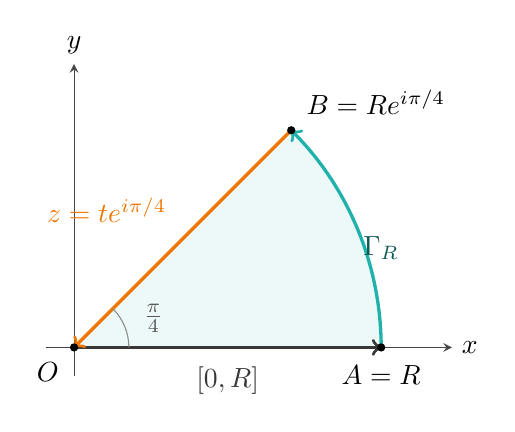
\begin{tikzpicture}[x=1.2cm,y=1.2cm,font=\normalsize]
    \draw[diagram axis] (-0.3,0)--(4.0,0) node[right] {$x$};
    \draw[diagram axis] (0,-0.3)--(0,3.0) node[above] {$y$};
    \coordinate (O) at (0,0);
    \coordinate (A) at (3.25,0);
    \coordinate (B) at ({3.25/sqrt(2)},{3.25/sqrt(2)});
    \fill[customcolor!8] (O)--(A) arc[start angle=0,end angle=45,radius=3.25]--cycle;
    \draw[very thick,black!78,->] (O)--(A) node[midway,below=3pt] {$[0,R]$};
    \draw[very thick,customcolor,->] (A) arc[start angle=0,end angle=45,radius=3.25];
    \draw[very thick,diagramorange,->] (B)--(O)
      node[midway,above left=2pt] {$z=te^{i\pi/4}$};
    \fill (O) circle (1.5pt) node[below left=2pt] {$O$};
    \fill (A) circle (1.5pt) node[below=3pt] {$A=R$};
    \fill (B) circle (1.5pt) node[above right=2pt] {$B=Re^{i\pi/4}$};
    \node[text=customcolor!50!black] at (3.25,1.05) {$\Gamma_R$};
    \draw[black!45] (0.58,0) arc[start angle=0,end angle=45,radius=0.58];
    \node[text=black!65] at (0.84,0.31) {$\frac{\pi}{4}$};
  \end{tikzpicture}
  \end{center}
  由 Cauchy 积分定理,
  \[
  \oint_{C}e^{-z^{2}}\,dz=\int_{\overrightarrow{OA}}e^{-z^{2}}\,dz+\int_{\Gamma_{R}}e^{-z^{2}}\,dz+\int_{\overrightarrow{BO}}e^{-z^{2}}\,dz=0,
  \]
  其中 $\int_{\overrightarrow{OA}}e^{-z^{2}}\,dz=\int_{0}^{R}e^{-x^{2}}\,dx$.
  在圆弧 $\Gamma_{R}:z=Re^{i\theta}$ ($0\leq\theta\leq\frac{\pi}{4}$) 上,
  \[
  \begin{aligned}
  \left|\int_{\Gamma_R}e^{-z^{2}}\,dz\right|
  &\leq R\int_{0}^{\pi/4}e^{-R^{2}\cos2\theta}\,d\theta\\
  &=\frac{R}{2}\int_{0}^{\pi/2}e^{-R^{2}\sin\varphi}\,d\varphi
  \leq\frac{R}{2}\int_{0}^{\pi/2}e^{-2R^{2}\varphi/\pi}\,d\varphi\\
  &=\frac{\pi}{4R}(1-e^{-R^{2}})<\frac{\pi}{4R}\longrightarrow0,
  \end{aligned}
  \]
  其中用到 $0\leq\varphi\leq\pi/2$ 时 $\sin\varphi\geq2\varphi/\pi$.
  对 $\overrightarrow{BO}$: $z=xe^{i\pi/4}$, $x$ 从 $R$ 到 $0$,
  \[
  \int_{\overrightarrow{BO}}e^{-z^{2}}\,dz
  =\int_{R}^{0}e^{i\pi/4}e^{-ix^{2}}\,dx
  =-e^{i\pi/4}\Bigl[\int_{0}^{R}\cos x^{2}\,dx-i\int_{0}^{R}\sin x^{2}\,dx\Bigr].
  \]
  令 $R\to+\infty$, 并用 $\int_{0}^{+\infty}e^{-x^{2}}\,dx=\frac{\sqrt{\pi}}{2}$, 得
  \[
  \int_{0}^{+\infty}e^{-x^{2}}\,dx-e^{i\pi/4}\Bigl[\int_{0}^{+\infty}\cos x^{2}\,dx-i\int_{0}^{+\infty}\sin x^{2}\,dx\Bigr]=0,
  \]
  即
  \[
  \int_{0}^{+\infty}\cos x^{2}\,dx-i\int_{0}^{+\infty}\sin x^{2}\,dx
  =e^{-i\pi/4}\frac{\sqrt{\pi}}{2}
  =\frac{\sqrt{\pi}}{2\sqrt{2}}(1-i).
  \]
  比较实部与虚部即得
  \[
  \int_{0}^{+\infty}\cos x^{2}\,dx=\int_{0}^{+\infty}\sin x^{2}\,dx=\frac{1}{2}\sqrt{\frac{\pi}{2}}.
  \]
\end{proof}

\begin{remark}
  还可用留数定理计算 $\int_{0}^{+\infty}\frac{\sin x}{x}\,dx=\frac{\pi}{2}$.
\end{remark}

\newpage

\section{辐角原理与儒歇定理}

问题: $\oint_{C}\frac{f'(z)}{f(z)}\,dz$ 的几何意义; $\operatorname{Res}\frac{f'(z)}{f(z)}$ 与 $C$ 内 $f(z)$ 极点、零点的关系.

\subsection{对数留数}

\begin{definition}
  设 $f(z)$ 在围线 $C$ 的某个邻域内解析，且在 $C$ 上非零, 称积分
  \[
  \frac{1}{2\pi i}\oint_{C}\frac{f'(z)}{f(z)}\,dz
  \]
  为 $f(z)$ 在 $C$ 上的对数留数.
\end{definition}

\begin{theorem}
  设 $f(z)$ 在围线 $C$ 上解析非零, 则
  \[
  \frac{1}{2\pi i}\oint_{C}\frac{f'(z)}{f(z)}\,dz=\frac{\Delta_{C}\arg f(z)}{2\pi},
  \]
  这里 $\frac{\Delta_{C}\arg f(z)}{2\pi}$ 表示当 $z$ 绕 $C$ 一周时其像曲线绕原点的环绕圈数.
\end{theorem}

\begin{proof}
  \[
  \frac{1}{2\pi i}\oint_{C}\frac{f'(z)}{f(z)}\,dz
  =\frac{1}{2\pi i}\oint_{C}d\ln f(z)
  =\frac{1}{2\pi i}\oint_{C}d\bigl(\ln|f(z)|+i\arg f(z)\bigr)
  =\frac{1}{2\pi i}\oint_{C}d\ln|f(z)|+\frac{1}{2\pi}\oint_{C}d\arg f(z)
  =0+\frac{\Delta_{C}\arg f(z)}{2\pi}.
  \]
\end{proof}

\begin{lemma}
  若 $f(z)$ 以 $z=a$ 为 $n$ 级零点, 则 $\frac{f'(z)}{f(z)}$ 以 $z=a$ 为一级极点, 且 $\operatorname{Res}_{z=a}\frac{f'(z)}{f(z)}=n$.
\end{lemma}

\begin{proof}
  $f(z)=(z-a)^{n}\varphi(z)$, $\varphi(a)\neq0$. 则
  \[
  \frac{f'(z)}{f(z)}=\frac{n(z-a)^{n-1}\varphi(z)+(z-a)^{n}\varphi'(z)}{(z-a)^{n}\varphi(z)}
  =\frac{n}{z-a}+\frac{\varphi'(z)}{\varphi(z)}.
  \]
  $\frac{\varphi'(z)}{\varphi(z)}$ 在 $z=a$ 解析, 故 $\frac{f'(z)}{f(z)}$ 以 $z=a$ 为一级极点, 留数为 $n$.
\end{proof}

\begin{lemma}
  若 $f(z)$ 以 $z=a$ 为 $m$ 级极点, 则 $\frac{f'(z)}{f(z)}$ 以 $z=a$ 为一级极点, 且 $\operatorname{Res}_{z=a}\frac{f'(z)}{f(z)}=-m$.
\end{lemma}

\begin{proof}
  $f(z)=\frac{\psi(z)}{(z-a)^{m}}$, $\psi(a)\neq0$. 则
  \[
  \frac{f'(z)}{f(z)}=\frac{\psi'(z)(z-a)^{m}-m(z-a)^{m-1}\psi(z)}{(z-a)^{2m}}\cdot\frac{(z-a)^{m}}{\psi(z)}
  =\frac{-m}{z-a}+\frac{\psi'(z)}{\psi(z)}.
  \]
  $\frac{\psi'(z)}{\psi(z)}$ 在 $z=a$ 解析, 故 $\frac{f'(z)}{f(z)}$ 以 $z=a$ 为一级极点, 留数为 $-m$.
\end{proof}

\subsection{辐角原理}

\begin{theorem}[辐角原理]
  设 $f(z)$ 在围线 $C$ 内除有限个极点外解析, 在 $C$ 上也解析且非零, 则
  \[
  \frac{\Delta_{C}\arg f(z)}{2\pi}=N(f,C)-P(f,C)=N-P.
  \]
  这里 $N$ 表示 $f(z)$ 在 $C$ 内零点总个数 ($n$ 级零点表示 $n$ 个零点),
  $P$ 表示 $f(z)$ 在 $C$ 内极点总个数 ($m$ 级极点表示 $m$ 个极点).
\end{theorem}

\begin{proof}
  $\frac{\Delta_{C}\arg f(z)}{2\pi}=\frac{1}{2\pi i}\oint_{C}\frac{f'(z)}{f(z)}\,dz$.
  记 $f(z)$ 在 $C$ 内零点 $a_{1},\cdots,a_{p}$ 与极点 $b_{1},\cdots,b_{q}$, 对应级为 $n_{1},\cdots,n_{p}$ 与 $m_{1},\cdots,m_{q}$.
  则 $\frac{f'(z)}{f(z)}$ 在 $C$ 内以 $a_{1},\cdots,a_{p},b_{1},\cdots,b_{q}$ 为一级极点.
  由留数定理,
  \[
  \frac{1}{2\pi i}\oint_{C}\frac{f'(z)}{f(z)}\,dz
  =\sum_{i=1}^{p}\operatorname{Res}_{z=a_{i}}\frac{f'(z)}{f(z)}
  +\sum_{i=1}^{q}\operatorname{Res}_{z=b_{i}}\frac{f'(z)}{f(z)}.
  \]
  由上述两引理,
  \[
  \sum_{i=1}^{p}\operatorname{Res}_{z=a_{i}}\frac{f'(z)}{f(z)}
  +\sum_{i=1}^{q}\operatorname{Res}_{z=b_{i}}\frac{f'(z)}{f(z)}
  =\sum_{i=1}^{p}n_{i}-\sum_{i=1}^{q}m_{i}=N-P.
  \]
\end{proof}

\begin{example}
  $f(z)=(z-1)(z-2)^{3}(z-4)$ 在 $|z|<3$ 上解析, 有 4 个零点, 则 $N-P=4$.
  沿 $|z|=3$ 逆时针转一圈时 $f(z)$ 绕原点转四圈.
\end{example}

\subsection{儒歇定理}

\begin{theorem}[Rouch\'{e} 定理]
  设 $f(z)$ 与 $\varphi(z)$ 在 $C$ 内解析, 在 $C$ 上解析且 $|f(z)|>|\varphi(z)|$,
  则 $f(z)$ 与 $f(z)\pm\varphi(z)$ 在 $C$ 内部有同样个数的零点.
\end{theorem}

\begin{proof}
  在 $C$ 上 $|f(z)|>0$, $\bigl|\frac{\varphi(z)}{f(z)}\bigr|<1$,
  \[
  \Delta_{C}\arg\bigl[f(z)\pm\varphi(z)\bigr]
  =\Delta_{C}\arg\Bigl[f(z)\Bigl(1\pm\frac{\varphi(z)}{f(z)}\Bigr)\Bigr]
  =\Delta_{C}\arg f(z)+\Delta_{C}\arg\Bigl(1\pm\frac{\varphi(z)}{f(z)}\Bigr)
  =\Delta_{C}\arg f(z)+0.
  \]
  由辐角原理, $N_{1}-P_{1}=N_{2}-P_{2}$ ($P_{1}=P_{2}=0$),
  于是 $N_{1}=N_{2}$, 其中 $N_{1},N_{2}$ 分别表示 $f(z)$ 和 $f(z)\pm\varphi(z)$ 在 $C$ 内的零点个数.
\end{proof}

\begin{example}
  (1) 方程 $z^{5}+8z^{3}+2z+1=0$ 在 $|z|<1$ 内有 3 个零点:
  取 $f(z)=8z^{3}$, $\varphi(z)=z^{5}+2z+1$, 在 $|z|=1$ 上 $|\varphi(z)|\leq4<8=|f(z)|$, 由 Rouch\'e 定理, $f(z)$ 在 $|z|<1$ 内有 3 个零点, 故原方程也有 3 个零点.

  (2) 方程 $z^{8}+7z^{2}+2z+19=0$ 在 $|z|<2$ 内有 8 个根:
  取 $f(z)=z^{8}$, $\varphi(z)=7z^{2}+2z+19$, 在 $|z|=2$ 上 $|\varphi/f|<1$, $f(z)$ 有 8 个零点, 故原方程在 $|z|<2$ 内也有 8 个根.
  取 $f(z)=19$, $\varphi(z)=z^{8}+7z^{2}+2z$, 在 $|z|=1$ 上 $|\varphi/f|<1$, 故 $|z|<1$ 内有 0 个根.

  (3) 任意 $n$ 次多项式方程 $z^{n}+a_{n-1}z^{n-1}+\cdots+a_{1}z+a_{0}=0$ 在复平面上有 $n$ 个根:
  取 $f(z)=z^{n}$, $\varphi(z)=a_{n-1}z^{n-1}+\cdots+a_{0}$, 当 $|z|$ 充分大时 $|f(z)|>|\varphi(z)|$, 故有 $n$ 个零点.
\end{example}

\newpage

\chapter{保形变换}

\section{解析函数的几何性质}

\begin{theorem}
  设 $f(z)$ 在区域 $D$ 上单叶解析, 则 $f'(z)\neq0$ ($\forall z\in D$).
\end{theorem}

\begin{proof}
  若 $\exists z_{0}\in D$ 使 $f'(z_{0})=0$, 则 $z_{0}$ 是 $f(z)-f(z_{0})$ 的 $n$ 级零点 ($n\geq2$). 此时 $z_{0}$ 也是 $f'(z)$ 的零点. 由零点的孤立性知,
  $\exists\rho>0$ 很小, 在 $|z-z_{0}|\leq\rho$ 上 $f(z)-f(z_{0})$ 与 $f'(z)$ 都只有 $z_{0}$ 一个零点.
  记 $\displaystyle\min_{|z-z_{0}|=\rho}|f(z)-f(z_{0})|=\delta>0$, 取 $0<|a|<\delta$.
  由 Rouch\'{e} 定理, $f(z)-f(z_{0})$ 与 $f(z)-f(z_{0})-a$ 在 $|z-z_{0}|<\rho$ 内有同样多的零点, 记作 $a_{1},\ldots,a_{n}$. 使 $f(a_{i})=f(z_{0})+a$.
  在 $0<|z-z_{0}|<\rho$ 内 $f'(z)\neq0$. 又因 $a\neq0$ 时 $a_i\neq z_0$, 故 $f'(a_{i})\neq0$,
  $a_{i}$ 是 $f(z)-f(z_{0})-a$ 的一级零点. 因此 $a_{1},\ldots,a_{n}$ 互不相等,
  与 $f(z)$ 在 $D$ 上单叶矛盾.
\end{proof}

\begin{remark}
  定理1的逆命题不成立. 反例: $f(z)=e^{z}$, $f'(z)=e^{z}\neq0$ 处处成立, 但 $f(z)$ 是周期函数, 不是单叶的.
\end{remark}

\begin{theorem}
  设 $f(z)$ 在区域 $D$ 内解析且 $\exists z_{0}\in D$ 使 $f'(z_{0})\neq0$, 则 $f(z)$ 在 $z_{0}$ 某邻域内单叶.
\end{theorem}

\begin{proof}
  $f(z)-f(z_{0})$ 以 $z_{0}$ 为一级零点, 由零点孤立性, $\exists\rho>0$ 使在 $|z-z_{0}|\leq\rho$ 上 $f(z)-f(z_{0})$ 只有 $z_{0}$ 一个零点.
  记 $\displaystyle\min_{|z-z_{0}|=\rho}|f(z)-f(z_{0})|=\delta>0$, $f(z_{0})=w^{*}$. 取 $m>0$ 使 $m<\delta$.
  对 $|w-w^{*}|<m$ 的 $w$, 由 Rouch\'{e} 定理, 在 $|z-z_{0}|<\rho$ 内 $f(z)-f(z_{0})$ 与 $f(z)-f(z_{0})-w+w^{*}=f(z)-w$ 有同样多个零点,
  前者只有一级零点 $z_0$，故后者恰有一个零点。即 $w^{*}$ 的 $m$ 邻域内
  任一 $w$ 都在 $|z-z_{0}|<\rho$ 内有唯一原像 $z$ 使 $f(z)=w$.
  由 $f(z)$ 在 $z_{0}$ 的连续性, $\exists z_{0}$ 的某邻域 $|z-z_{0}|<r<\rho$ 使 $f(z)$ 全落在 $w^{*}$ 的 $m$ 邻域内, 此时 $f(z)$ 在该邻域上单叶.
\end{proof}

\subsection{解析函数的保域性}

\begin{theorem}[保域性定理]
  设 $f(z)$ 在区域 $D$ 上解析且非常数, 则其像集 $G=f(D)$ 也是区域.
\end{theorem}

\begin{proof}
  (1) 先证 $G=f(D)$ 中每个点都是内点. 任取 $w^{*}\in f(D)$, 记 $f(z_{0})=w^{*}$.
  $f(z)-f(z_{0})$ 以 $z_{0}$ 为零点, 由零点孤立性, $\exists\rho>0$ 使 $f(z)-f(z_{0})$ 在 $|z-z_{0}|\leq\rho$ 上没有除 $z_{0}$ 外的其他零点.
  记 $\displaystyle\min_{|z-z_{0}|=\rho}|f(z)-f(z_{0})|=\delta>0$, 取 $m>0$ 使 $m<\delta$. 对 $|w-w^{*}|<m$, 在 $|z-z_{0}|=\rho$ 上由 Rouch\'{e} 定理,
  在 $|z-z_{0}|<\rho$ 内 $f(z)-f(z_{0})$ 与 $f(z)-f(z_{0})-w+w^{*}=f(z)-w$ 有同样多的零点,
  即 $w^{*}$ 的 $m$ 邻域中每个 $w$ 都是 $w=f(z)$ 的像, 表明 $w^{*}$ 是 $f(D)$ 的内点, 进而 $f(D)$ 是开集.

  (2) 下证 $f(D)$ 连通. 任取 $w_{1},w_{2}\in f(D)$, 对应 $z_{1},z_{2}\in D$ 使 $f(z_{1})=w_{1}$, $f(z_{2})=w_{2}$.
  记 $C$ 是 $D$ 内连接 $z_{1}$ 与 $z_{2}$ 的折线, $C$ 在变换 $w=f(z)$ 下的像曲线 $\Gamma=f(C)$ 是连续曲线且 $\Gamma\subset f(D)$.
  由 (1), $\Gamma=f(C)$ 上的点都是 $f(D)$ 的内点, 故 $\exists$ $f(D)$ 的子区域 $G_{1}$ 使 $\Gamma\subset G_{1}$.
  于是在区域 $G_{1}$ 内可作 $w_{1},w_{2}$ 间折线, 即 $w_{1},w_{2}$ 可用折线连通, $f(D)$ 为区域.
\end{proof}

\begin{corollary}[最大模原理]
  若 $f(z)$ 在区域 $D$ 解析且非常数, 则 $|f(z)|$ 在 $D$ 内取不到最大值.
\end{corollary}

\begin{proof}
  由保域性定理, $f(D)$ 是区域, 若 $|f(z)|$ 在 $z_{0}\in D$ 取最大值, 则 $f(z_{0})$ 不是 $f(D)$ 的内点, 矛盾.
\end{proof}

\subsection{导数的几何意义}

设 $f(z)$ 在 $z_{0}$ 解析, 且 $f'(z_{0})=Re^{i\alpha}\neq0$.

\begin{enumerate}
  \item 导数辐角 $\alpha$ 的几何意义——旋转角:\par
  设 $C$ 是从 $z_{0}$ 出发的光滑曲线, $C:z=z(t)$, $z(t_{0})=z_{0}$, $z'(t_{0})$ 表示 $C$ 在 $z_{0}$ 的切向量.\par
  $C$ 在变换 $w=f(z)$ 下的像曲线: $\Gamma=f(C)$, $w=w(t)=f(z(t))$. $w(t_{0})=f(z_{0})$, $w'(t_{0})$ 是 $\Gamma$ 的切向量, 则有:
  \[
  \arg w'(t_{0})=\arg f'(z_{0})+\arg z'(t_{0}).
  \]
  即 $\alpha=\arg f'(z_{0})$ 是将过 $z_{0}$ 的曲线的切向量旋转的角度. 称 $\alpha=\arg f'(z_{0})$ 为 $w=f(z)$ 在 $z_{0}$ 的\textbf{旋转角}.

  进而, 过 $z_{0}$ 的两条曲线 $C_{1},C_{2}$ 在变换 $w=f(z)$ 下的像曲线 $\Gamma_{1},\Gamma_{2}$ 的夹角与 $C_{1},C_{2}$ 的夹角大小相等、方向相同, 即变换 $w=f(z)$ 在 $z_{0}$ 具有\textbf{保角性}.

  \item 导数模 $R$ 的几何意义——伸缩率:\par
  $|f'(z_{0})|=\lim_{\Delta z\to0}\frac{|\Delta w|}{|\Delta z|}=R$, 表示 $f(z)$ 在 $z_{0}$ 处的伸缩率, 即像曲线在 $w_{0}$ 的线元长度与原曲线在 $z_{0}$ 的线元长度之比的极限. 称 $R$ 为 $w=f(z)$ 在 $z_{0}$ 的\textbf{伸缩率}.
\end{enumerate}

\subsection{保形变换}

\begin{definition}
  设 $f(z)$ 在 $z_{0}$ 邻域内连续, 且变换 $w=f(z)$ 在 $z_{0}$ 点保角且保伸缩率, 则称变换 $w=f(z)$ 在 $z_{0}$ 保形.
\end{definition}

\begin{definition}
  若变换 $w=f(z)$ 在区域 $D$ 上处处保角, 则称变换 $w=f(z)$ 在区域 $D$ 上保角.
\end{definition}

\begin{definition}
  若变换 $w=f(z)$ 在区域 $D$ 上单叶保角, 则称变换 $w=f(z)$ 是 $D$ 上的保形变换 (共形映射).
\end{definition}

\begin{theorem}
  单叶解析变换一定是保形变换 ($f'(z)\neq0$ 保角、保伸缩率). 单叶解析变换的逆变换也是保形变换.
\end{theorem}

\begin{theorem}[保形变换的解析性]
  区域 $D$ 上的保形变换 $w=f(z)$ 一定是解析函数对应的变换.
\end{theorem}

\begin{remark}
  保角变换中保角性可以推出保伸缩性.
\end{remark}

\newpage

\section{分式线性变换}

\subsection{线性变换的定义}

\begin{definition}
  有理分式函数
  \[
  w=L(z)=\frac{az+b}{cz+d}\quad\Bigl(\begin{vmatrix}a&b\\c&d\end{vmatrix}\neq0\Bigr)
  \]
  对应的变换称为分式线性变换, 简称线性变换.\par
  逆变换: $z=\frac{-dw+b}{cw-a}$, 也是线性变换.
\end{definition}

在变换 $w=\frac{az+b}{cz+d}$ 中:
\begin{enumerate}
  \item 当 $c\neq0$ 时, $z=-\frac{d}{c}$ 对应 $w=\infty$; $z=\infty$ 对应 $w=\frac{a}{c}$.
  \item 当 $c=0$ 时, $w=\frac{a}{d}z+\frac{b}{d}$, $z=\infty$ 对应 $w=\infty$.
\end{enumerate}
这样, 线性变换建立了扩充 $z$ 平面到扩充 $w$ 平面的一一映射.

\subsection{分式线性变换的分解}

\begin{enumerate}
  \item 当 $c\neq0$ 时, $w=\frac{az+b}{cz+d}=\frac{a}{c}+\frac{bc-ad}{c(cz+d)}$.
  \item 当 $c=0$ 时, $w=\frac{a}{d}z+\frac{b}{d}$.
\end{enumerate}
这样, 线性变换 $w=\frac{az+b}{cz+d}$ 可看成下面两种变换的复合:
\begin{itemize}
  \item I: $w=az+b$ (整线性变换)
  \item II: $w=\frac{1}{z}$ (反演变换)
\end{itemize}

整线性变换 $w=az+b$ 的几何性质: 记 $a=\rho e^{i\alpha}$, $z=re^{i\theta}$, 则 $w=\rho re^{i(\alpha+\theta)}+b$, 几何上可以看成伸缩、旋转、平移的复合. 例如, 整线性变换将直线变为直线; 将三角形变为相似三角形.

反演变换 $w=\frac{1}{z}$ 的几何性质: $w=\frac{1}{z}$ 可以看成 $w=\overline{w_{1}}$, $w_{1}=\frac{1}{\overline{z}}$, 即先关于单位圆对称再关于实轴对称.

\subsection{线性变换的性质}

\begin{enumerate}
  \item 保形性:\par
  整线性变换 $w=az+b$ 保形 ($\frac{dw}{dz}=a\neq0$).\par
  反演变换 $w=\frac{1}{z}$ 保形 ($\frac{dw}{dz}=-\frac{1}{z^{2}}\neq0$).\par
  定义曲线在 $\infty$ 点的夹角: 将过 $\infty$ 的两光滑曲线用反演变换变为过原点的两条曲线的夹角, 称为两曲线在 $\infty$ 的夹角.\par
  于是整线性变换 $w=az+b$ 在 $z=\infty$ 保角; 反演变换 $w=\frac{1}{z}$ 在 $z=0$ 保角, 在 $z=\infty$ 也保角.\par
  综上, 线性变换 $w=\frac{az+b}{cz+d}$ 在扩充平面上保角.

  \item 保圆性: 线性变换将圆周(或直线)变为圆周(或直线).\par
  \begin{proof}
    (1) 在整线性变换下, 圆周的像显然是圆周, 直线的像显然是直线.\par
    (2) 在反演变换 $w=\frac{1}{z}$ 下, 设原曲线 $\gamma$ 的方程: $A z\overline{z}+B z+\overline{B}\overline{z}+C=0$,
    其中 $A=0$ 时表示直线, $A\neq0$ 时表示圆周.\par
    在变换下, $\gamma$ 的像 $\Gamma=L(\gamma)$ 的方程:
    $C w\overline{w}+\overline{B}w+B\overline{w}+A=0$.\par
    当 $C=0$ 时 $\Gamma$ 表示直线, $C\neq0$ 时 $\Gamma$ 表示圆周.\par
    总结: 若将直线看成半径为 $\infty$ 的圆, 则线性变换保圆性.
  \end{proof}
  \item 保交比性:\par
  \begin{definition}
    四个复数的交比定义为
    \[
    (z_{1},z_{2},z_{3},z_{4})=\frac{z_{4}-z_{1}}{z_{4}-z_{2}}:\frac{z_{3}-z_{1}}{z_{3}-z_{2}}.
    \]
  \end{definition}

  \begin{theorem}
    线性变换 $w=\frac{az+b}{cz+d}$ 下, 记 $w_{i}=\frac{az_{i}+b}{cz_{i}+d}$ ($i=1,2,3,4$), 则
    \[
    (w_{1},w_{2},w_{3},w_{4})=(z_{1},z_{2},z_{3},z_{4}).
    \]
  \end{theorem}

  \begin{proof}
    \[
    w_{i}-w_{j}=\frac{az_{i}+b}{cz_{i}+d}-\frac{az_{j}+b}{cz_{j}+d}
    =\frac{(ad-bc)(z_{i}-z_{j})}{(cz_{i}+d)(cz_{j}+d)},
    \]
    代入交比定义即得 $(w_{1},w_{2},w_{3},w_{4})=(z_{1},z_{2},z_{3},z_{4})$.
  \end{proof}

  \begin{remark}
    四个复数中一个可以为 $\infty$, 例如:
    \[
    (\infty,z_{2},z_{3},z_{4})=\frac{1}{z_{4}-z_{2}}:\frac{1}{z_{3}-z_{2}},\qquad
    (z_{1},z_{2},z_{3},\infty)=1:\frac{z_{3}-z_{1}}{z_{3}-z_{2}}.
    \]
    线性变换 $w=\frac{az+b}{cz+d}$ 中四个系数只有三个独立.
  \end{remark}

  \begin{example}
    求线性变换 $w=L(z)$ 使 $z=2,i,-2$ 分别对应 $w=-1,i,1$.

    根据线性变换保交比性,
    \[
    \frac{w+1}{w-i}:\frac{1+1}{1-i}=\frac{z-2}{z-i}:\frac{-2-2}{-2-i},
    \]
    解出 $w=\dfrac{z-6i}{3iz-2}$.
  \end{example}

  \item 保对称性:\par
  \begin{definition}
    (1) 平面中两点 $z_{1},z_{2}$ 关于直线 $l$ 对称: 若 $l$ 将线段 $z_{1}z_{2}$ 垂直平分.\par
    (2) 平面中两点 $z_{1},z_{2}$ 关于圆周 $|z-a|=R$ 对称: $z_{1},z_{2}$ 在过圆心 $a$ 的同一条射线上, 且 $|z_{2}-a||z_{1}-a|=R^{2}$.\par
    补充规定: 圆心关于圆周的对称点为 $\infty$.
  \end{definition}

  \begin{theorem}
    设 $\gamma$ 是 $z$ 平面上一条圆周或直线, $z_{1},z_{2}$ 关于 $\gamma$ 对称, 在线性变换 $w=L(z)$ 下,
    记 $w_{1}=L(z_{1})$, $w_{2}=L(z_{2})$, $\Gamma=L(\gamma)$, 则 $w_{1},w_{2}$ 关于 $\Gamma=L(\gamma)$ 对称.
  \end{theorem}
\end{enumerate}

\newpage

\section{常见的保形变换举例}

\subsection{上半平面到上半平面的线性变换}

特点:
\begin{enumerate}
  \item 三个有序实数 $x_{1}<x_{2}<x_{3}$ 对应 $w$ 平面上三个有序实数 $w_{1}<w_{2}<w_{3}$, 由保交比性有对应线性变换:
  \[
  (z,x_{1},x_{2},x_{3})=(w,w_{1},w_{2},w_{3}).
  \]
  \item 该变换满足: $w=\frac{az+b}{cz+d}$, 四个系数可以均为实数; $w'(x)=\frac{ad-bc}{(cx+d)^{2}}>0$.
\end{enumerate}

类似地, 上半平面到下半平面的线性变换:
\begin{enumerate}
  \item 若 $x_{1}<x_{2}<x_{3}$, 则 $w_{1}>w_{2}>w_{3}$.
  \item $w=\frac{az+b}{cz+d}$, 四个系数可以均为实数; $w'(x)=\frac{ad-bc}{(cx+d)^{2}}<0$.
\end{enumerate}

\begin{example}
  求上半平面到上半平面的线性变换 $w=w(z)$, 满足 $w(i)=1+i$, $w(0)=0$.

  \textbf{解法1:} 根据保对称性, $w(-i)=1-i$, 根据保交比性可求.

  \textbf{解法2:} 设所求变换 $w=\frac{az+b}{cz+d}$, $a,b,c,d\in\mathbb{R}$.
  由 $w(0)=0$ 得 $b=0$, $w=\frac{az}{cz+d}=\frac{z}{ez+f}$, $e,f\in\mathbb{R}$.
  再由 $w(i)=1+i$, 得 $1+i=\frac{i}{ei+f}\Rightarrow e=f=\frac{1}{2}$.
  故所求变换 $w=\frac{2z}{z+1}$.
\end{example}

\subsection{上半平面到单位圆的线性变换}

已知上半平面中一点 $a$ ($\operatorname{Im}a>0$) 变为 $w=0$ ($\overline{a}\to\infty$),
所求变换具有形式 $w=k\cdot\frac{z-a}{z-\overline{a}}$, 由 $|w(0)|=1$ 知 $|k|=1$, 即 $k=e^{i\alpha}$, 其中 $\alpha$ 为待求参数.
故
\[
w=e^{i\alpha}\frac{z-a}{z-\overline{a}},\quad \operatorname{Im}a>0.
\]

若 $\arg w'(a)=\beta$ 已知, 则
\[
w'(z)=e^{i\alpha}\cdot\frac{a-\overline{a}}{(z-\overline{a})^{2}},\qquad
w'(a)=e^{i\alpha}\cdot\frac{1}{a-\overline{a}},
\]
\[
\beta=\arg w'(a)=\alpha+\arg\Bigl(\frac{1}{a-\overline{a}}\Bigr)=\alpha+\arg\Bigl(\frac{1}{i}\Bigr)=\alpha-\frac{\pi}{2},
\]
故 $\alpha=\frac{\pi}{2}+\beta$.

\begin{example}
  确定将 $z=\frac{i}{2}$ 变为 $w=0$ 且将上半平面变为单位圆的线性变换, 若 $\arg w'(\frac{i}{2})=\frac{\pi}{2}$.
  \[
  w=e^{\pi i}\cdot\frac{z-\frac{i}{2}}{z+\frac{i}{2}}=-\frac{z-\frac{i}{2}}{z+\frac{i}{2}}.
  \]
\end{example}

\subsection{单位圆到单位圆的线性变换}

已知 $|a|<1$ 且 $w(a)=0$ ($\frac{1}{\overline{a}}\to\infty$),
所求变换 $w=k\cdot\frac{z-a}{z-\frac{1}{\overline{a}}}=k_{1}\cdot\frac{z-a}{1-\overline{a}z}$.
再由 $|w(1)|=1$, 得 $|k_{1}|=1$. 故
\[
w=e^{i\alpha}\frac{z-a}{1-\overline{a}z},\quad |a|<1.
\]

若 $\arg w'(a)=\beta$ 已知, 则 $\alpha=\beta$.

\begin{example}
  若单位圆 $|z|<1$ 到 $|w|<1$ 的线性变换 $w=L(z)$ 满足 $L(\frac{1}{2})=0$, 且 $\arg w'(\frac{1}{2})=\pi$, 则
  \[
  L(z)=e^{i\pi}\cdot\frac{z-\frac{1}{2}}{1-\frac{1}{2}z}=-\frac{2z-1}{2-z}.
  \]
\end{example}

\subsection{指数函数与对数函数所成变换}

$w=e^{z}$ 在单叶性区域 $0<\operatorname{Im}z<2\pi$ 内保形, 其像区域为去掉正实轴的平面.
一般地, $z$ 平面上带形域 $0<\operatorname{Im}z<y_{0}$ 变为角形域 $0<\arg w<y_{0}$.
特别地, 宽度为 $\pi$ 的带形域 $0<\operatorname{Im}z<\pi$ 变为上半平面.
同理, $w=\ln z$ 将角形域变为带形域 (主值支).

\begin{example}
  求带形域 $0<\operatorname{Im}z<\pi$ 变为单位圆 $|w|<1$ 的保形变换, 满足 $w(\frac{\pi i}{2})=0$, 且 $\arg\bigl(w'(\frac{\pi i}{2})\bigr)=\pi$.

  (1) $w_{1}=e^{z}$ 变为上半平面 $\operatorname{Im}w_{1}>0$, 且 $\frac{\pi i}{2}\to i$.\par
  (2) $w=e^{i\alpha}\frac{w_{1}-i}{w_{1}+i}$ 将上半平面变为单位圆, 由 $\arg w'(\frac{\pi i}{2})=\pi$ 得 $\alpha=\pi$.\par
  复合有: $w=-\dfrac{e^{z}-i}{e^{z}+i}$.
\end{example}

\subsection{幂函数与根式函数所成变换}

$n\in\mathbb{N}^{+}$. $w=z^{\frac{1}{n}}$ 的单叶性区域: $0<\arg z<2\pi$, 变为 $0<\arg w<\frac{2\pi}{n}$.
$w=z^{n}$ 将 $0<\arg z<\frac{2\pi}{n}$ 变为 $0<\arg w<2\pi$.

\begin{example}
  求将角域 $0<\arg z<\frac{\pi}{2}$ 变为上半平面的保形变换 $w=w(z)$, 使 $w(e^{\frac{\pi}{4}i})=1+i$ 且 $w(0)=0$.

  (1) $w_{1}=z^{2}$ 变为上半平面, $w_{1}(e^{\frac{\pi}{4}i})=i$, $w_{1}(0)=0$.\par
  (2) 将 $i\to1+i$, $0\to0$ 的上半平面到上半平面变换: $w=\frac{2w_{1}}{w_{1}+1}$.\par
  复合后有 $w=\dfrac{2z^{2}}{z^{2}+1}$.
\end{example}

\subsection{其他保形变换举例}

两个相交的圆弧所围成的单连域变为上半平面或单位圆.
可通过线性变换 $w=k\dfrac{z-a}{z-b}$ 变为角形域, 然后用幂函数变为上半平面.

\begin{center}
\begin{tikzpicture}[x=1.1cm,y=1.1cm,font=\normalsize]
  \coordinate (a) at (-4.7,0);
  \coordinate (b) at (-2.0,0);
  \fill[customcolor!11]
    (a) .. controls (-4.05,1.05) and (-2.65,1.05) .. (b)
        .. controls (-2.55,-0.68) and (-4.15,-0.68) .. cycle;
  \draw[customcolor,very thick]
    (a) .. controls (-4.05,1.05) and (-2.65,1.05) .. (b);
  \draw[diagramorange,very thick]
    (a) .. controls (-4.15,-0.68) and (-2.55,-0.68) .. (b);
  \fill (a) circle (1.5pt) node[left=3pt] {$a$};
  \fill (b) circle (1.5pt) node[right=3pt] {$b$};
  \node[text=customcolor!50!black] at (-3.35,0.18) {$D$};

  \draw[diagram map] (-1.48,0)--(0.65,0)
    node[midway,above=5pt] {$w=k\dfrac{z-a}{z-b}$};

  \coordinate (V) at (1.35,0);
  \fill[customcolor!10] (V)--(4.55,0)--(4.1,1.58)--cycle;
  \draw[diagram axis] (0.95,0)--(4.78,0) node[below right] {$\operatorname{Re}w$};
  \draw[diagram axis] (1.35,-0.75)--(1.35,1.9) node[above] {$\operatorname{Im}w$};
  \draw[diagramorange,very thick] (V)--(4.55,0);
  \draw[customcolor,very thick] (V)--(4.1,1.58);
  \draw[black!45] (2.0,0) arc[start angle=0,end angle=30,radius=0.65];
  \node[text=black!65] at (2.15,0.33) {$\alpha$};
  \node[text=customcolor!50!black] at (3.25,0.62) {$L(D)$（角形域）};
\end{tikzpicture}
\end{center}

\begin{example}
  求一个将上半单位圆 $|z|<1$, $\operatorname{Im}z>0$ 变为上半平面的保形变换.

  (1) 线性变换 $w_{1}=-\frac{z+1}{z-1}$ 将上半单位圆变为第一象限 $0<\arg w_{1}<\frac{\pi}{2}$.\par
  (2) 所求变换 $w=w_{1}^{2}=\bigl(-\frac{z+1}{z-1}\bigr)^{2}$.
\end{example}

\newpage

\section{保形变换的存在唯一性定理}

\begin{theorem}
  设 $D$ 与 $G$ 分别是扩充 $z$ 平面和扩充 $w$ 平面上两个边界不止一点的单连域, 其间存在保形变换 $w=w(z)$. 若给定 $z_{0}\in D$, $w_{0}\in G$, $w(z_{0})=w_{0}$ 且 $\arg w'(z_{0})=\alpha$, 则该变换唯一.
\end{theorem}

\begin{proof}
  略.
\end{proof}

\begin{corollary}
  设 $D$ 是扩充 $z$ 平面上边界不止一点的单连域, 则存在保形变换 $w=f(z)$ 使 $f(D)$ 为单位圆. 若 $z_{0}\in D$ 使 $f(z_{0})=0$ 且 $\arg f'(z_{0})=\alpha$, 则该变换唯一.
\end{corollary}

\begin{remark}
  ``边界不止一点'': 若单连域是扩充复平面去掉 $\infty$ 一点, 则 $w=f(z)$ 将平面变为单位圆,
  即 $|f(z)|<1$, 由 Liouville 定理 $f(z)$ 必为常数, 矛盾.
  若去掉 $z=a$ 一点, 则也不存在单叶解析函数 $w=f(z)$ 将之变为单位圆.
  因若存在, 则 $w_{1}=\frac{1}{z-a}$ 将去点平面变为去 $\infty$ 平面, 再复合即矛盾.
\end{remark}

\begin{theorem}
  设 $D$ 与 $G$ 分别是 $z$ 平面和 $w$ 平面上两个分别以简单闭曲线 $C$ 和 $\Gamma$ 为边界的有界单连域.
  若 $w=f(z)$ 在 $D$ 上解析, 在 $D\cup C$ 上连续, 且 $w=f(z)$ 将 $C$ 双方单值变为 $\Gamma$ 且保形,
  则 $w=f(z)$ 在 $D$ 内单叶解析.
\end{theorem}

\end{document}
